\pdfoutput=1
\documentclass{article}

\usepackage{microtype}

% if you need to pass options to natbib, use, e.g.:

    \PassOptionsToPackage{numbers, compress}{natbib}
% before loading neurips_2024


% ready for submission
\usepackage[main, final]{neurips_2026}
\usepackage{multirow}
\newcommand*\rot{\rotatebox{90}}

%Adjust the format of task
\renewcommand\ttdefault{cmtt}


% to compile a preprint version, e.g., for submission to arXiv, add add the
% [preprint] option:
% \usepackage[preprint]{neurips_2024}


% to compile a camera-ready version, add the [final] option, e.g.:
% \usepackage[final]{neurips_2024}
\usepackage{multirow}


% to avoid loading the natbib package, add option nonatbib:
% \usepackage[nonatbib]{neurips_2024}
\usepackage{caption}
% \usepackage{subcaption}
\usepackage[utf8]{inputenc} % allow utf-8 input
\usepackage[T1]{fontenc}    % use 8-bit T1 fonts
\usepackage{lmodern}

\usepackage{adjustbox}

% \usepackage{hyperref}       % hyperlinks
\usepackage{url}            % simple URL typesetting
\usepackage{booktabs}       % professional-quality tables
\usepackage{amsfonts}       % blackboard math symbols
\usepackage{nicefrac}       % compact symbols for 1/2, etc.
\usepackage{
microtype}      % microtypography
% \usepackage{xcolor}         % colors
% \usepackage{natbib}
\usepackage{amsmath}
\usepackage{amssymb}
\usepackage{mathtools}
% \numberwithin{equation}{section}
\usepackage{slashed}
\usepackage{braket}
\usepackage{enumitem}
\usepackage{bbm}
\usepackage[svgnames]{xcolor}
\usepackage[colorlinks,citecolor=DarkGreen,linkcolor=FireBrick,urlcolor=FireBrick,linktocpage=true,unicode]{hyperref}
\usepackage{multirow}
\usepackage{subcaption}
\usepackage{graphicx}
\allowdisplaybreaks
% \usepackage{cite}
\usepackage{graphicx}
\usepackage{tikz}
\usepackage{tikz-cd}
\usepackage{times}
\renewcommand\ttdefault{cmtt} 
\usepackage{bm}
\usepackage{physics}
\usepackage{xcolor}
\usepackage{natbib}
\usepackage{mdframed}
\usepackage{nicefrac}
\usepackage{booktabs}
\usepackage{lipsum}
\usepackage{titlesec}
\usepackage{wrapfig,lipsum,booktabs}
\usepackage{authblk}
\usepackage{blindtext}
\usepackage{subcaption}

\usepackage{algorithm}
\usepackage{algpseudocode}
% Algorithm definitions
\newcommand{\commentsymbol}{//}% or \% or $\triangleright$
\algrenewcommand\algorithmiccomment[1]{\hfill {\footnotesize \commentsymbol{} #1}}




\usepackage{titletoc}
\usepackage{todonotes}
\usepackage{authblk}
\usepackage{setspace}
\usepackage{dsfont} % for \mathbb{1} as \mathds{1}
\newcommand{\one}{\mathds{1}}

%%% Section Notation %%%
\usepackage[nameinlink,capitalize,noabbrev]{cleveref}
% \crefformat{section}{\S#2#1#3} % see manual of cleveref, section 8.2.1
% \crefformat{subsection}{\S#2#1#3}
% \crefformat{subsubsection}{\S#2#1#3}
% \crefformat{appendix}{\S #2#1#3}
% use: See \cref{sec:section}, \cref{sec:subsection} or \cref{sec:subsubsection}
%%% Section Notation %%%

%%% Chinese ###
\usepackage{CJK}
\newcommand{\zh}[1]{\begin{CJK}{UTF8}{bsmi}\normalfont\small #1\end{CJK}} % 繁體中文
\newcommand{\zhs}[1]{\begin{CJK}{UTF8}{gbsn}\normalfont \small#1\end{CJK}}% 簡體中文 
%%%% \begin{CJK}{UTF8}{bsmi}\normalfont 中文\end{CJK} when word missing %%%

%%%Claim%%%
\newenvironment{claim}{  \begin{mdframed}[linecolor=black!0,backgroundcolor=black!10]\noindent%\itshape
		\ignorespaces}{\end{mdframed}}

% \let\originalfigure=\figure
% \let\endoriginalfigure=\endfigure

% \renewenvironment{figure}[1][]{
%   \begin{originalfigure}[#1]
%     \begin{mdframed}[linecolor=black!0,backgroundcolor=black!1]
% }{
%     \end{mdframed}
%   \end{originalfigure}
% }
%%%Claim%%%

%%%% skip line in table %%%
\usepackage{array}
\usepackage{bbm}
\usepackage{makecell}

\renewcommand\theadalign{bc}
\renewcommand\theadfont{\bfseries}
\renewcommand\theadgape{\Gape[4pt]}
\renewcommand\cellgape{\Gape[0pt]}
%%%% skip line in table %%%

%% Comment%%
\newcommand{\jerry}[1]{\textcolor{red}{[JH: #1]}}
% \newcommand{\matt}[1]{\textcolor{firebrick}{[Matthew: #1]}}
\newcommand{\smj}[1]{\textcolor{blue}{[MJ: #1]}}
\newcommand{\zqj}[1]{\textcolor{red}{QZ: #1}}
% \newcommand{\juihui}[1]{\textcolor{magenta}{[juihui: #1]}}



\def\half{{\frac{1}{2}}}

%

\usepackage{dashbox}
\usepackage{xcolor}
\usepackage{colortbl}
\definecolor{lightyellow}{rgb}{1.0, 0.95, 0.7}
% \definecolor{Blue}{rgb}{0, 0.18, 0.65}
\definecolor{Blue}{rgb}{0, 0, 0.8}
\definecolor{blue}{rgb}{0,0,1}
% \definecolor{darkgreen}{rgb}{0.01,0.50,0.2}
\definecolor{darkgreen}{rgb}{0,0.40,0}
\definecolor{firebrick}{rgb}{0.698,0.133,0.133}
\newcommand*{\red}[1]{\textcolor{red}{#1}}
\newcommand*{\Red}[1]{\textcolor{firebrick}{#1}}
\newcommand*{\Blue}[1]{\textcolor{Blue}{#1}}
\newcommand*{\blue}[1]{\textcolor{blue}{#1}}
\newcommand*{\green}[1]{\textcolor{darkgreen}{#1}}
\newcommand*{\black}[1]{\textcolor{black}{#1}}

\definecolor{colorA}{rgb}{1,0,0}
\definecolor{colorB}{rgb}{0,0.3,1}
\definecolor{colorC}{rgb}{0.9,0.8,0.2}
\definecolor{colorD}{rgb}{0,0.65,0}
\definecolor{lesslightgray}{rgb}{0.5,0.5,0.5}
\definecolor{light-gray}{gray}{0.95}
\newcommand{\code}[1]{\colorbox{light-gray}{\footnotesize\texttt{#1}}}
\newcommand*{\grey}[1]{\textcolor{black!50}{#1}}
\newcommand*{\colorA}[1]{\textcolor{colorA}{#1}}
\newcommand*{\colorB}[1]{\textcolor{colorB}{#1}}
\newcommand*{\colorC}[1]{\textcolor{colorC}{#1}}
\newcommand*{\colorD}[1]{\textcolor{colorD}{#1}}


\let\tilde\widetilde
\let\hat\widehat

\newcommand{\calA}{\mathcal{A}}
\newcommand{\calB}{\mathcal{B}}
\newcommand{\calC}{\mathcal{C}}
\newcommand{\calD}{\mathcal{D}}
\newcommand{\calE}{\mathcal{E}}
\newcommand{\calF}{\mathcal{F}}
\newcommand{\calG}{\mathcal{G}}
\newcommand{\calH}{\mathcal{H}}
\newcommand{\calI}{\mathcal{I}}
\newcommand{\calJ}{\mathcal{J}}
\newcommand{\calK}{\mathcal{K}}
\newcommand{\calL}{\mathcal{L}}
\newcommand{\calM}{\mathcal{M}}
\newcommand{\calN}{\mathcal{N}}
\newcommand{\calO}{\mathcal{O}}
\newcommand{\calP}{\mathcal{P}}
\newcommand{\calQ}{\mathcal{Q}}
\newcommand{\calR}{\mathcal{R}}
\newcommand{\calS}{\mathcal{S}}
\newcommand{\calT}{\mathcal{T}}
\newcommand{\calU}{\mathcal{U}}
\newcommand{\calV}{\mathcal{V}}
\newcommand{\calW}{\mathcal{W}}
\newcommand{\calX}{\mathcal{X}}
\newcommand{\calY}{\mathcal{Y}}
\newcommand{\calZ}{\mathcal{Z}}




% \newcommand{\bA}{\mathbf{A}}
% \newcommand{\bB}{\mathbf{B}}
% \newcommand{\bC}{\mathbf{C}}
% \newcommand{\bD}{\mathbf{D}}
% \newcommand{\bE}{\mathbf{E}}
% \newcommand{\bF}{\mathbf{F}}
% \newcommand{\bG}{\mathbf{G}}
% \newcommand{\bH}{\mathbf{H}}
% \newcommand{\bI}{\mathbf{I}}
% \newcommand{\bJ}{\mathbf{J}}
% \newcommand{\bK}{\mathbf{K}}
% \newcommand{\bL}{\mathbf{L}}
% \newcommand{\bM}{\mathbf{M}}
% \newcommand{\bN}{\mathbf{N}}
% \newcommand{\bO}{\mathbf{O}}
% \newcommand{\bP}{\mathbf{P}}
% \newcommand{\bQ}{\mathbf{Q}}
% \newcommand{\bR}{\mathbf{R}}
% \newcommand{\bS}{\mathbf{S}}
% \newcommand{\bT}{\mathbf{T}}
% \newcommand{\bU}{\mathbf{U}}
% \newcommand{\bV}{\mathbf{V}}
% \newcommand{\bW}{\mathbf{W}}
% \newcommand{\bX}{\mathbf{X}}
% \newcommand{\bY}{\mathbf{Y}}
% \newcommand{\bZ}{\mathbf{Z}}
% \newcommand{\ba}{\mathbf{a}}
% \newcommand{\bb}{\mathbf{b}}
% \newcommand{\bc}{\mathbf{c}}
% \newcommand{\bd}{\mathbf{d}}
% \newcommand{\be}{\mathbf{e}}
% \newcommand{\bk}{\mathbf{k}}
% \newcommand{\bmf}{\mathbf{f}}
% \newcommand{\bu}{\mathbf{u}}
% \newcommand{\bp}{\mathbf{p}}
% \newcommand{\bs}{\mathbf{s}}
% \newcommand{\bg}{\mathbf{g}}
% \newcommand{\bh}{\mathbf{h}}
% \newcommand{\br}{\mathbf{r}}
% \newcommand{\bv}{\mathbf{v}}
% \newcommand{\bq}{\mathbf{q}}
% \newcommand{\bx}{\mathbf{x}}
% \newcommand{\by}{\mathbf{y}}
% \newcommand{\bz}{\mathbf{z}}
% \newcommand{\bxi}{{\bm{\xi}}}
\newcommand{\diag}{\mathop{\rm{diag}}}
\newcommand{\Max}{\mathop{\rm Max}}
\newcommand{\Min}{\mathop{\rm Min}}
\newcommand{\argmin}{\mathop{\mathrm{argmin}}}  
\newcommand{\argmax}{\mathop{\mathrm{argmax}}}  
\newcommand{\Var}{\mathop{\mathrm{Var}}}
\newcommand{\Sigmoid}{\mathop{\rm{Sigmoid}}}
\newcommand{\Softmax}{\mathop{\rm{Softmax}}}
\newcommand{\Sparsemax}{\mathop{\rm{Sparsemax}}}
\newcommand{\Sign}{\mathop{\rm{Sign}}}
\newcommand{\lse}{\mathop{\rm{lse}}}



\newcommand{\sumN}{\sum_{i=1}^N}
\newcommand{\sumK}{\sum_{k=1}^K}
\newcommand{\sumq}{\sum_{k=1}^q}
\newcommand{\summ}{\sum_{i=1}^m}
\newcommand{\sumM}{\sum_{\mu=1}^M}
\newcommand{\sumn}{\sum_{i=1}^n}
\newcommand{\sumd}{\sum_{i=1}^d}
\newcommand{\sumT}{\sum_{t=1}^T}

\def\P{\mathbb{P}}
\def\R{\mathbb{R}}
\def\B{\mathbb{B}}
%\def\E{\mathbb{E}}
\DeclareMathOperator*{\E}{{\mathbb{E}}} %%Zhao: I added this
\def\I{\mathcal{I}}
\def\p{\partial }
\let\cite\citep 

%%%%%%%%%%%%%%%%%%%%%%%%%%%%%%%%%%%%%%%%%%
\usepackage{amsthm}
\usepackage[many]{tcolorbox}
\setlength{\topsep}{0.8\baselineskip}  % Reduce space before and after theorems
\setlength{\partopsep}{\topsep}        % Consistent spacing for partopsep
% Adjust proof environment spacing manually
\usepackage{etoolbox}
% half‑baseline gap before every proof
\BeforeBeginEnvironment{proof}{\par\vspace{-1\baselineskip}}
% half‑baseline gap after every proof (and end the paragraph)
\AfterEndEnvironment  {proof}{\par\vspace{-1.5\baselineskip}}





% Adjusting spacing for all theorem-like environments
\newtheoremstyle{theoremstyle}
  {.5\baselineskip} % Space above
  {.5\baselineskip} % Space below
  {}                  % No font styling for body
  {}                  % Indentation
  {\bfseries}        % Heading font
  {.}                 % Punctuation
  {1em}               % Space after heading
  {}                  % Extra customization


\theoremstyle{theoremstyle}
\newtheorem{theorem}{Theorem}[section]
\newtheorem{lemma}{Lemma}[section]
\newtheorem{corollary}{Corollary}[theorem]
\newtheorem{proposition}{Proposition}[section]
\newtheorem{definition}{Definition}[section]
\newtheorem{assumption}{Assumption}[section]
\newtheorem{remark}{Remark}[section]
\newtheorem{problem}{Problem}
\newtheorem{property}{Property}

\tcolorboxenvironment{theorem}{
  breakable,
  colback=black!10,
  colframe=white,%
  width=\dimexpr\linewidth+10pt\relax,%  
  enlarge left by=-5pt,%                  
  enlarge right by=-5pt,%                 
  boxsep=5pt,%            
  boxrule=0pt,
  left=0pt,right=0pt,top=0pt,bottom=0pt,
  sharp corners,
  before skip=0.5\baselineskip, % Reduced space above
  after skip=0.5\baselineskip,  % Reduced space below
  fonttitle=\bfseries, % Bold title for theorem
  coltitle=black % Black title color
}
\tcolorboxenvironment{remark}{
  blanker,
  breakable,
  before skip=.8\baselineskip,  % half a baseline above
  after  skip=.8\baselineskip   % half a baseline below
}

\tcolorboxenvironment{proposition}{
  breakable,
  colback=black!10,
  colframe=white,%
  width=\dimexpr\linewidth+10pt\relax,%  
  enlarge left by=-5pt,%                  
  enlarge right by=-5pt,%                 
  boxsep=5pt,%            
  boxrule=0pt,
  left=0pt,right=0pt,top=0pt,bottom=0pt,
  sharp corners,
  before skip=0.5\baselineskip, % Reduced space above
  after skip=0.5\baselineskip,  % Reduced space below
  fonttitle=\bfseries, % Bold title for theorem
  coltitle=black % Black title color
}

\tcolorboxenvironment{lemma}{
  breakable,
  colback=black!10,
  colframe=white,%
  width=\dimexpr\linewidth+10pt\relax,%  
  enlarge left by=-5pt,%                  
  enlarge right by=-5pt,%                 
  boxsep=5pt,%            
  boxrule=0pt,
  left=0pt,right=0pt,top=0pt,bottom=0pt,
  sharp corners,
  before skip=0.5\baselineskip, % Reduced space above
  after skip=0.5\baselineskip,  % Reduced space below
  fonttitle=\bfseries, % Bold title for theorem
  coltitle=black % Black title color
}

\tcolorboxenvironment{corollary}{
  breakable,
  colback=black!10,
  colframe=white,%
  width=\dimexpr\linewidth+10pt\relax,%  
  enlarge left by=-5pt,%                  
  enlarge right by=-5pt,%                 
  boxsep=5pt,%            
  boxrule=0pt,
  left=0pt,right=0pt,top=0pt,bottom=0pt,
  sharp corners,
  before skip=0.5\baselineskip, % Reduced space above
  after skip=0.5\baselineskip,  % Reduced space below
  fonttitle=\bfseries, % Bold title for theorem
  coltitle=black % Black title color
}

\tcolorboxenvironment{definition}{
  breakable,
  colback=black!10,
  colframe=white,%
  width=\dimexpr\linewidth+10pt\relax,%  
  enlarge left by=-5pt,%                  
  enlarge right by=-5pt,%                 
  boxsep=5pt,%            
  boxrule=0pt,
  left=0pt,right=0pt,top=0pt,bottom=0pt,
  sharp corners,
  before skip=0.5\baselineskip, % Reduced space above
  after skip=0.5\baselineskip,  % Reduced space below
  fonttitle=\bfseries, % Bold title for theorem
  coltitle=black % Black title color
}
\tcolorboxenvironment{assumption}{
  breakable,
  colback=black!10,
  colframe=white,%
  width=\dimexpr\linewidth+10pt\relax,%  
  enlarge left by=-5pt,%                  
  enlarge right by=-5pt,%                 
  boxsep=5pt,%            
  boxrule=0pt,
  left=0pt,right=0pt,top=0pt,bottom=0pt,
  sharp corners,
  before skip=0.5\baselineskip, % Reduced space above
  after skip=0.5\baselineskip,  % Reduced space below
  fonttitle=\bfseries, % Bold title for theorem
  coltitle=black % Black title color
}

\crefname{theorem}{Theorem}{Theorems}
\crefname{proposition}{Proposition}{Propositions}
\crefname{lemma}{Lemma}{Lemmas}
\crefname{corollary}{Corollary}{Corollaries}
\crefname{definition}{Definition}{Definitions}
\crefname{assumption}{Assumption}{Assumptions}
\crefname{remark}{Remark}{Remarks}
\crefname{problem}{Problem}{Problems}
\crefname{property}{Property}{property}
\newtheorem{hypothesis}{Hypothesis}
\tcolorboxenvironment{hypothesis}{
  breakable,
  colback=black!10,
  colframe=white,%
  width=\dimexpr\linewidth+10pt\relax,%  
  enlarge left by=-5pt,%                  
  enlarge right by=-5pt,%                 
  boxsep=5pt,%            
  boxrule=0pt,
  left=0pt,right=0pt,top=0pt,bottom=0pt,
  sharp corners,
  before skip=0.5\baselineskip, % Reduced space above
  after skip=0.5\baselineskip,  % Reduced space below
  fonttitle=\bfseries, % Bold title for theorem
  coltitle=black % Black title color
}
\crefname{hypothesis}{Hypothesis}{Hypothesises}

\newtheorem{fact}{Fact}
\tcolorboxenvironment{fact}{
  breakable,
  colback=black!10,
  colframe=white,%
  width=\dimexpr\linewidth+10pt\relax,%  
  enlarge left by=-5pt,%                  
  enlarge right by=-5pt,%                 
  boxsep=5pt,%            
  boxrule=0pt,
  left=0pt,right=0pt,top=0pt,bottom=0pt,
  sharp corners,
  before skip=0.5\baselineskip, % Reduced space above
  after skip=0.5\baselineskip,  % Reduced space below
  fonttitle=\bfseries, % Bold title for theorem
  coltitle=black % Black title color
}
\crefname{fact}{Fact}{Facts}

\newtheorem{example}{Example}
\tcolorboxenvironment{example}{
  breakable,
  colback=black!10,
  colframe=white,%
  width=\dimexpr\linewidth+10pt\relax,%  
  enlarge left by=-5pt,%                  
  enlarge right by=-5pt,%                 
  boxsep=5pt,%            
  boxrule=0pt,
  left=0pt,right=0pt,top=0pt,bottom=0pt,
  sharp corners,
  before skip=0.5\baselineskip, % Reduced space above
  after skip=0.5\baselineskip,  % Reduced space below
  fonttitle=\bfseries, % Bold title for theorem
  coltitle=black % Black title color
}
\crefname{example}{Example}{Examples}

\newtheorem{question}{Question}
\tcolorboxenvironment{question}{
  breakable,
  colback=black!10,
  colframe=white,%
  width=\dimexpr\linewidth+10pt\relax,%  
  enlarge left by=-5pt,%                  
  enlarge right by=-5pt,%                 
  boxsep=5pt,%            
  boxrule=0pt,
  left=0pt,right=0pt,top=0pt,bottom=0pt,
  sharp corners,
  before skip=0.5\baselineskip, % Reduced space above
  after skip=0.5\baselineskip,  % Reduced space below
  fonttitle=\bfseries, % Bold title for theorem
  coltitle=black % Black title color
}






\crefname{question}{Question}{Questions}
\numberwithin{equation}{section}
\numberwithin{theorem}{section}
\numberwithin{proposition}{section}
\numberwithin{definition}{section}
\numberwithin{lemma}{section}
\numberwithin{assumption}{section}
\numberwithin{remark}{section}

%=== footnote without marker ===
% \blfootnote[]{}
\usepackage{lipsum}

\newcommand\blfootnote[1]{%
  \begingroup
  \renewcommand\thefootnote{}\footnote{#1}%
  \addtocounter{footnote}{-1}%
  \endgroup
}
%=== footnote without marker ===
%%% derivation step description
\newcommand*{\annot}[1]{\tag*{\footnotesize{\textcolor{black!50}{\big(#1\big)}}}}

%%% Better Bar Notation%%%
\makeatletter
\let\save@mathaccent\mathaccent
\newcommand*\if@single[3]{%
    \setbox0\hbox{${\mathaccent"0362{#1}}^H$}%
    \setbox2\hbox{${\mathaccent"0362{\kern0pt#1}}^H$}%
    \ifdim\ht0=\ht2 #3\else #2\fi
}
%The bar will be moved to the right by a half of \macc@kerna, which is computed by amsmath:
\newcommand*\rel@kern[1]{\kern#1\dimexpr\macc@kerna}
%If there's a superscript following the bar, then no negative kern may follow the bar;
%an additional {} makes sure that the superscript is high enough in this case:
\newcommand*\widebar[1]{\@ifnextchar^{{\wide@bar{#1}{0}}}{\wide@bar{#1}{1}}}
%Use a separate algorithm for single symbols:
\newcommand*\wide@bar[2]{\if@single{#1}{\wide@bar@{#1}{#2}{1}}{\wide@bar@{#1}{#2}{2}}}
\newcommand*\wide@bar@[3]{%
    \begingroup
    \def\mathaccent##1##2{%
        %Enable nesting of accents:
        \let\mathaccent\save@mathaccent
        %If there's more than a single symbol, use the first character instead (see below):
        \if#32 \let\macc@nucleus\first@char \fi
        %Determine the italic correction:
        \setbox\z@\hbox{$\macc@style{\macc@nucleus}_{}$}%
        \setbox\tw@\hbox{$\macc@style{\macc@nucleus}{}_{}$}%
        \dimen@\wd\tw@
        \advance\dimen@-\wd\z@
        %Now \dimen@ is the italic correction of the symbol.
        \divide\dimen@ 3
        \@tempdima\wd\tw@
        \advance\@tempdima-\scriptspace
        %Now \@tempdima is the width of the symbol.
        \divide\@tempdima 10
        \advance\dimen@-\@tempdima
        %Now \dimen@ = (italic correction / 3) - (Breite / 10)
        \ifdim\dimen@>\z@ \dimen@0pt\fi
        %The bar will be shortened in the case \dimen@<0 !
        \rel@kern{0.6}\kern-\dimen@
        \if#31
        \overline{\rel@kern{-0.6}\kern\dimen@\macc@nucleus\rel@kern{0.4}\kern\dimen@}%
        \advance\dimen@0.4\dimexpr\macc@kerna
        %Place the combined final kern (-\dimen@) if it is >0 or if a superscript follows:
        \let\final@kern#2%
        \ifdim\dimen@<\z@ \let\final@kern1\fi
        \if\final@kern1 \kern-\dimen@\fi
        \else
        \overline{\rel@kern{-0.6}\kern\dimen@#1}%
        \fi
    }%
    \macc@depth\@ne
    \let\math@bgroup\@empty \let\math@egroup\macc@set@skewchar
    \mathsurround\z@ \frozen@everymath{\mathgroup\macc@group\relax}%
    \macc@set@skewchar\relax
    \let\mathaccentV\macc@nested@a
    %The following initialises \macc@kerna and calls \mathaccent:
    \if#31
    \macc@nested@a\relax111{#1}%
    \else
    %If the argument consists of more than one symbol, and if the first token is
    %a letter, use that letter for the computations:
    \def\gobble@till@marker##1\endmarker{}%
    \futurelet\first@char\gobble@till@marker#1\endmarker
    \ifcat\noexpand\first@char A\else
    \def\first@char{}%
    \fi
    \macc@nested@a\relax111{\first@char}%
    \fi
    \endgroup
    }
\makeatother
\let\bar\widebar


\usepackage{tocloft}   % <-- add this in the preamble, BEFORE you set lengths

% Adjust the spacing in the table of contents
\setlength{\cftbeforesecskip}{2pt} % Space before section entries
\setlength{\cftbeforesubsecskip}{0pt} % Space before subsection entries
\setlength{\cftbeforesubsubsecskip}{0pt} % Space before subsubsection entries


\newcommand{\indep}{\mathbin{\perp\!\!\!\perp}}

%Adjust Space of Section
\titlespacing*{\section}{0pt}{0pt}{0pt}
\titlespacing*{\subsection}{0pt}{0pt}{0pt}
\titlespacing*{\subsubsection}{0pt}{0pt}{0pt}

% % Compact spacing for sections
% \titlespacing{\section}{0pt}{*1}{*-1}
% % More compact spacing for subsections
% \titlespacing{\subsection}{0pt}{*1}{*-1}
% \titlespacing{\subsubsection}{0pt}{*1}{*-1}
% \titlespacing{\paragraph}{0pt}{*1}{1em} % Adjust last value for horizontal space after paragraph title


\usepackage{titletoc}

\newcommand{\ie}{\mbox{\it{i.e.,\ }}}
\newcommand{\eg}{\mbox{
\it{e.g.,\ }}}


\def\algorithmautorefname{Algorithm}
\def\equationautorefname{Equation}
\def\Snospace~{\S{}}
\renewcommand*\sectionautorefname{\Snospace}
\def\sectionautorefname{\Snospace}
\def\subsectionautorefname{\Snospace}
\def\subsubsectionautorefname{\Snospace}
\def\chapterautorefname{\Snospace}
\newcommand{\sref}[2]{\hyperref[#2]{#1 \ref{#2}}}
% use autoref for most cases. For assumptions, lemma, theorem, etc., use \sref. For example, \sref{Assumption}{assumption:random}
\newcommand{\cms}[1]{{\color{purple} \small \sf $\ll$Minshuo: {#1}$\gg$}}


\title{Doob-Based Generative Policy Optimization }


% The \author macro works with any number of authors. There are two commands
% used to separate the names and addresses of multiple authors: \And and \AND.
%
% Using \And between authors leaves it to LaTeX to determine where to break the
% lines. Using \AND forces a line break at that point. So, if LaTeX puts 3 of 4
% authors names on the first line, and the last on the second line, try using
% \AND instead of \And before the third author name.
\vspace{-1.2em}

\author{
\textbf{
Maojiang Su$^{\dagger,\natural}$
\hspace{0.7em}
Qijie Zhu$^{\ddag}$
\hspace{0.7em}
Yu Xiao
$^{\dagger}$
\hspace{0.7em}
Shuyang Yu$^{\dagger}$
}
\\
\vspace{-0.7em}
\textbf{
Minshuo Chen$^{\S}$
\hspace{0.7em}
Zhaoran Wang$^{\S,\dagger}$
\hspace{0.7em}
Han Liu$^{\dagger,\ddag,\natural}$
}
\\
\vspace{0.7em}
\begin{minipage}{0.95\textwidth}
\raggedright
\small
$^{\dagger\;}$Department of Computer Science,
Northwestern University, Evanston, IL 60208, USA
\\
$^{\ddag\;}$Department of Statistics and Data Science,
Northwestern University, Evanston, IL 60208, USA
\\
$^{\S\;}$Department of Industrial Engineering and Management Sciences,
\\
\hphantom{$^{\S\;}$}Northwestern University, Evanston, IL 60208, USA
\\
$^{\natural\;}$Center for Foundation Models and Generative AI,
Northwestern University, Evanston, IL 60208, USA
\end{minipage}
\\
\vspace{0.45em}
{\footnotesize
\href{https://maojiangsu.github.io/DoobPO/}
{\texttt{https://maojiangsu.github.io/DoobPO/}}
}
}
\vspace{0.5em}

% \setlength{\abovedisplayskip}{4pt}
% \setlength{\abovedisplayshortskip}{4pt}
% \setlength{\belowdisplayskip}{4pt}
% \setlength{\belowdisplayshortskip}{4pt}
% \setlength{\abovedisplayskip}{10pt}
% \setlength{\belowdisplayskip}{10pt}

\setlist[itemize]{
  leftmargin=1em,
  topsep=0.5pt,
  itemsep=2pt,
  parsep=0pt,
  partopsep=0pt
}

\setlist[enumerate]{
  leftmargin=1.4em,
  topsep=0.5pt,
  itemsep=2pt,
  parsep=0pt,
  partopsep=0pt
}
% \setlist[itemize]{leftmargin=1em}
% \setlist[enumerate]
% {leftmargin=1.4em}

%Adjust space of proof env
\BeforeBeginEnvironment{proof}{\par\vspace{-0.4\baselineskip}}
% half‑baseline gap after every proof (and end the paragraph)
\AfterEndEnvironment  {proof}{\par\vspace{-0.4\baselineskip}}

\titlespacing{\paragraph}{0pt}{0.1ex}{0.3em}



\begin{document}
\setlength{\abovedisplayskip}{2pt}
\setlength{\abovedisplayshortskip}{2pt}
\setlength{\belowdisplayskip}{2pt}
\setlength{\belowdisplayshortskip}{2pt}

\maketitle
\vspace{-2.2em}
\begin{abstract}
\vspace{-1.5em}
Diffusion and flow models provide expressive policy classes for robotic and sequential decision-making systems.
However, their action likelihoods are generally intractable, limiting the direct use of widely adopted policy optimization methods such as PPO and GRPO. We propose Doob Policy Optimization (DoobPO), a framework that leverages  Doob's $h$-transform for likelihood-free reinforcement learning fine-tuning of generative policies. DoobPO separates policy improvement from generative policy learning. It first learns a lightweight ratio model that represents the desired policy update, and then distills the resulting ratio-tilted target policy into the generative policy via conditional drift matching. This formulation applies uniformly to both diffusion and flow policies and supports a broad family of policy improvement rules, including PPO and GRPO. 
We prove that the practical conditional drift matching objective is gradient-equivalent to the ideal Doob drift matching objective. 
We further show that the induced diffusion process solves an endpoint-constrained stochastic optimal control problem. This establishes that it achieves the minimum-energy modification required to realize the desired policy tilt.
Across MuJoCo continuous-control benchmarks, DoobPO achieves strong performance against competitive diffusion- and flow-policy baselines,  showing a principled and practical route to RL fine-tuning for generative policies.
\end{abstract}

\section{Introduction}
\label{sec:intro}

Generative policies based on diffusion models
\cite{song2019generative,song2020score,ho2020denoising}
and flow matching models
\cite{lipman2022flow,liu2022flow}
have emerged as a powerful paradigm for policy learning.
Diffusion policies generate actions through iterative denoising, while flow policies generate actions by integrating a learned velocity field, often providing a deterministic and more efficient alternative.
Due to their flexibility and accuracy in modeling high-dimensional action distributions, generative policies have achieved strong empirical gains over deterministic or unimodal policies in challenging continuous-control settings
\cite{ke20243d,chi2025diffusion,huang2024diffuseloco,black2024pi,intelligence2025pi}.

A natural way to further improve generative policies is through reinforcement learning fine-tuning.
However, a central challenge is that the exact likelihoods of generative policies are generally intractable, since each action is produced only after simulating an entire denoising or flow trajectory.
This prevents the direct use of many stable and widely adopted policy optimization methods, such as PPO
\cite{schulman2017proximal}
and GRPO
\cite{shao2024deepseekmath}.
Several recent works have attempted to bypass this likelihood challenge
\cite{psenka2023learning,ding2024diffusion,ma2025efficient,ren2024diffusion,zhang2025reinflow,mcallister2025flow}.
However, these methods often suffer from biased estimation, limited data efficiency, substantial computational overhead, or restriction to a particular generative policy class or policy update rule.
Consequently, the full potential of RL for diffusion and flow policies remains underexplored.

To address this problem, we propose \textbf{Doob Policy Optimization (DoobPO)}, a likelihood-free framework that separates policy improvement from generative policy learning.
The first stage represents the desired policy improvement through a target policy ratio.
The second stage distills the resulting ratio-tilted target into the generative policy.
This decomposition avoids evaluating the likelihood of the generative policy itself.
The policy-improvement stage is agnostic to the underlying generative model and accommodates a broad family of updates, including regularized Policy Mirror Descent~\cite{zhan2023policy}, Soft Actor-Critic~\cite{haarnoja2018soft}, PPO~\cite{schulman2017proximal}, and GRPO~\cite{shao2024deepseekmath}.
The generative stage uses Doob's $h$-transform to characterize the ratio-tilted target process and learns this process through Doob's Drift Matching.
The same construction applies to both diffusion and flow policies.

\textbf{Contributions.}
Our contributions are three-fold:
\begin{itemize}
    \item \textbf{Method.}
    We propose \textbf{Doob Policy Optimization (DoobPO)}, a unified framework for RL fine-tuning of generative policies without evaluating exact action likelihoods
    (\cref{sec:method}).
    DoobPO follows a two-stage design: it first obtains the target policy ratio and then transfers the resulting policy improvement into the generative policy through a tractable conditional drift matching objective.
    The framework supports both diffusion and flow policies
    (\cref{sec:diff_dr_matching,sec:flow_dr_matching}).
    We summarize
    the procedures in
    \cref{alg:rwdm_ppo,alg:rwdm_ppo_fm}.
    Instantiating DoobPO with different policy updates yields
    \textbf{DoobPMD}, \textbf{DoobPPO}, and \textbf{DoobGRPO}.
    We further show that several existing methods arise as special cases under particular choices of the policy update and generative policy class
    (\cref{sec:unified_framework}).
    We summarize these instantiations in \Cref{tab:unified_framework}.

    \item \textbf{Theory.}
    We characterize the ratio-tilted target policy through Doob's $h$-transform
    (\cref{lem:algo_correctness}).
    This characterization leads to Doob's Drift Matching as a principled way to realize the desired policy update.
    For tractability, we introduce a conditional drift matching objective and prove that its gradient is proportional to that of the ideal Doob's Drift Matching objective for both diffusion and flow policies
    (\cref{thm:grad_equi_diff,thm:grad_equi_fm}).
    From the Stochastic Optimal Control perspective
    (\cref{sec:soc}),
    we further show that the Doob-transformed diffusion solves the corresponding endpoint-constrained control problem
    (\cref{prop:cdm_solves_soc}).
    Hence, DoobPO learns the minimum-energy modification of the pretrained diffusion process that realizes the terminal tilt
    (\cref{rem:ratio_h_interpretation}).

    \item \textbf{Experiments.}
    We evaluate DoobPO on MuJoCo continuous-control benchmarks with both diffusion and flow policies
    (\cref{sec:exp}).
    For diffusion policies, DoobPO achieves the strongest overall performance against competitive diffusion-policy RL baselines, with leading results on most tasks
    (\cref{sec:diffusion_exp}).
    For flow policies, DoobGRPO achieves the best performance on 9 out of 10 tasks under the same interaction budget and delivers large gains on challenging locomotion environments
    (\cref{sec:flow_exp}).
    These results establish DoobPO as a strong and practical framework for RL fine-tuning across both diffusion and flow policies.
\end{itemize}

\textbf{Notation.}
We summarize notation and time conventions in \cref{sec:notation}.

\textbf{Related Work.}
We defer an extended discussion of related work to \cref{sec:related_works} due to page limits.


\section{Preliminaries}
\label{sec:background}


\textbf{Reinforcement Learning.}
We formulate the task by defining a Markov Decision Process (MDP) \cite{sutton1998reinforcement} with a tuple $(\mathcal{S}, \mathcal{A}, P, R, \gamma)$.
Here, $\mathcal{S}$ and $\mathcal{A}$ denote the state and action spaces.
We use $o \in \mathcal{S}$ to denote a state and $a \in \mathcal{A}$ to denote an action.
The transition kernel is denoted by $P(o' | o,a)$, the reward function by $R(o,a)$,
and $\gamma \in [0,1)$ is the discount factor.
A policy $\pi(a | o)$ induces a distribution over trajectories
$\tau = (o_0,a_0,o_1,a_1,\ldots)$, where $a_t \sim \pi(\cdot | o_t)$
and $o_{t+1} \sim P(\cdot | o_t,a_t)$.
The standard objective of RL is to maximize
\begin{align}
\label{eq:rl_objective_prelim}
    J(\theta)
    =
    \E_{\tau \sim d_{\pi_\theta}(\tau)}
    \Big[
    \sum_{t \ge 0} \gamma^t R(o_t,a_t)
\Big],
\end{align}
where $d_{\pi_\theta}(\tau)$ is the distribution of trajectories generated by the policy $\pi_\theta$ and the transition kernel.
Policy gradient methods (e.g., REINFORCE \cite{williams1992simple}) update $\theta$ by ascending an estimate of $\nabla_\theta J(\theta)$,
\begin{align}
\label{eq:policy_gradient}
    \nabla_\theta J(\theta)
    =
    \E_{\tau \sim d_{\pi_\theta}(\tau)}
    \Big[\sum_{t\ge 0} \gamma^t
        \nabla_\theta \log \pi_\theta(a_t | o_t)
        \sum_{k\ge t}\gamma^{k-t} R(o_k,a_k)
    \Big],
\end{align}
where $\nabla_\theta \log \pi_\theta(a_t | o_t)$ is the score function of the policy.
To reduce variance, we often replace the cumulative future reward $\sum_{k\ge t}\gamma^{k-t} R(o_k,a_k)$ with an advantage estimate $A(o_t,a_t)$.

In practice, directly optimizing \eqref{eq:policy_gradient}
may be unstable due to overly large policy updates.
Trust-region style policy gradient methods \cite{schulman2015trust,schulman2017proximal,shao2024deepseekmath} instead constrain the policy change between successive iterates.
A popular example is Proximal Policy Optimization (PPO) \cite{schulman2017proximal}, which maximizes $J_{\mathrm{PPO}}(\theta)$
\begin{align}
    \E_{\tau \sim d_{\pi_{\text{old}}}(\tau)}
    \Big[
        \sum_{t\ge 0}
        \min\Big(
            r_\theta(o_t,a_t)\hat{A}_{\mathrm{old}}(o_t,a_t),
            \mathrm{clip}\big(r_\theta(o_t,a_t),1-\epsilon,
            1+\epsilon\big)\hat{A}_{\mathrm{old}}(o_t,a_t)
        \Big)
    \Big],
    \label{eq:ppo}
\end{align}
where $\pi_{\mathrm{old}}$ is the behavior policy, $r_\theta(o,a):=\pi_\theta(a|o)/\pi_{\mathrm{old}}(a|o)$ is the probability ratio, $\epsilon>0$ is the clipping parameter, and $\hat{A}_{\mathrm{old}}(o,a)$ is an advantage estimator.
The clipped surrogate upweights actions that are estimated to be better than baseline and limits the policy update away from $\pi_{\mathrm{old}}$.

\begin{table*}[t]
\centering
\caption{\small Doob Policy Optimization}
\label{tab:unified_framework}
\resizebox{0.8\linewidth}{!}{%
\begin{tabular}{l|ccc}
\toprule
Method
& Generative policy
& Policy update method
& Ratio
\\
\midrule
DPMD \cite{ma2025efficient}
& Diffusion
& Policy Mirror Descent (KL-proximal)
& Analytic
\\

SDAC \cite{ma2025efficient}
& Diffusion
& Soft Actor Critic
& Analytic
\\

DoobPMD (ours)
& Flow
& Policy Mirror Descent (KL-proximal)
& Analytic
\\

DoobPPO (ours)
& Diffusion / Flow
& Proximal Policy Optimization
& Learned
\\

DoobGRPO (ours)
& Diffusion / Flow
& Group Relative Policy Optimization
& Learned
\\
\bottomrule
\end{tabular}}
% \vspace{-2em}
\end{table*}




\textbf{Diffusion Models and Score Matching.}
Let $p_0$ denote the data distribution.
Diffusion models define a forward noising process
$(Y_t)_{t \in [0,T]}$ that gradually transforms data
into noise through the Stochastic Differential Equation
(SDE) \cite{song2020score}
\begin{align}
\label{eq:forward_sde}
    \dd Y_t
    =
    f(Y_t,t)\dd t
    +
    \sigma_t\dd W_t,
    \quad
    Y_0 \sim p_0,
    \quad
    t \in [0,T],
\end{align}
where $f$ and $\sigma_t$ are pre-designed drift and
diffusion coefficients, and $W_t$ is a standard
Brownian motion.
We denote by $p_t$ the marginal distribution of $Y_t$.
The generative process is the reverse-time denoising
process $(X_t)_{t \in [0,T]}$, evolving from $t=T$
to $t=0$.
It transports noise back to data, with
$X_T \sim p_T$ and $X_0 \sim p_0$.
Its time-$t$ marginal is $p_t$, and the process
is governed by the reverse-time SDE
\begin{align}
\label{eq:reverse_sde}
    \dd X_t
    =
    \bigl[
        f(X_t,t)
        -
        \sigma_t^2 \nabla_x \log p_t(X_t)
    \bigr]\dd t
    +
    \sigma_t \dd \overline W_t,
    \quad
    X_T \sim p_T,
    \quad
    t:T \to 0.
\end{align}
Here, $\overline W_t$ denotes a Wiener process in
the reverse-time direction.

Directly using \eqref{eq:reverse_sde} is difficult
in practice because the noise distribution $p_T$
and the true score $\nabla_x \log p_t$ are not
known explicitly.
Therefore, \eqref{eq:reverse_sde} is implemented
through two approximations.
First, the noise distribution $p_T$ is approximated
by a standard Gaussian distribution.
Second, the ground-truth score function
$s(x,t) := \nabla_x \log p_t(x)$
is replaced by a parameterized estimator
$s_\phi(x,t)$.
The score estimator is learned by minimizing
the score matching loss
\begin{align}
\label{eq:score_matching}
    \mathcal{L}_{\mathrm{SM}}(\phi)
    =
    \E_{t, Y_t \sim p_t}
    \bigl[
        \|s(Y_t,t) - s_\phi(Y_t,t)\|_2^2
    \bigr].
\end{align}


\textbf{Flow Matching.}
Following the notation in \cite{lipman2024flow}, let $p_0$ denote the noise distribution and $p_T$ the data distribution (opposite to the diffusion convention).
Flow matching constructs a deterministic transport from $p_0$ to $p_T$ via the Ordinary Differential Equation (ODE)
\begin{align}
\label{eq:fm_ode}
    \dd X_t = u(X_t,t)\dd t,
\end{align}
where $u(x,t)$ is the velocity field and $p_t$ denotes the marginal probability density function of $X_t$.
Given a reference velocity $u(x,t)$ that induces the desired path $\{p_t\}_{t\in[0,T]}$, flow matching learns a parameterized velocity $u_\phi(x,t)$ by minimizing
the flow matching loss
\begin{align}
\label{eq:flow_matching}
    \mathcal{L}_{\mathrm{FM}}(\phi)
    =
    \E_{t, X_t \sim p_t}
    \Big[\big\| u(X_t,t) - u_\phi(X_t,t)\big\|_2^2\Big].
\end{align}
After training, new samples are generated by simulating the ODE \eqref{eq:fm_ode} from $t=0$ to $t=T$, replacing the unknown velocity $u(x,t)$ with its learned estimator $u_\phi(x,t)$.


\textbf{Diffusion Policy and Flow Policy.}
A diffusion policy \cite{chi2025diffusion} is a policy induced by a diffusion model.
Let $s_\phi(x,t)$ be a parameterized score network, and let
$\{p_t^\phi\}_{t\in[0,T]}$ denote the marginal distributions obtained by
simulating the reverse-time SDE \eqref{eq:reverse_sde} with the score
$\nabla_x \log p_t(x)$ replaced by $s_\phi(x,t)$.
The diffusion policy $\pi_\phi$ is defined as the distribution over actions induced at the terminal time of the denoising process,
$\pi_\phi(\cdot|o) = p_0^\phi(\cdot|o)$.
A flow policy \cite{black2024pi,intelligence2025pi} is a policy induced by a flow matching model.
Let $u_\phi(x,t)$ be a parameterized velocity field, and let
$\{p_t^\phi\}_{t\in[0,T]}$ denote the marginals obtained by simulating the ODE \eqref{eq:fm_ode} with $u(x,t)$ replaced by $u_\phi(x,t)$.
The flow policy $\pi_\phi$ is defined as the action distribution at the terminal time of the flow, i.e.,
$\pi_\phi(\cdot|o)=p_T^\phi(\cdot|o)$.

For both diffusion and flow policies, evaluating the likelihood $\pi_\phi(a|o)$ is expensive.
As a result, the probability ratio
$\pi_\phi(a|o)/\pi_{\mathrm{old}}(a|o)$ in trust-region policy gradient methods (e.g., PPO, GRPO) is intractable.
This limits applying these methods to improve diffusion and flow policies.
DoobPO overcomes this obstacle and enables stable policy gradient style optimization for generative policies.


\section{Doob-Based Generative Policy Optimization}
\label{sec:method}

We introduce \textbf{Doob Policy Optimization (DoobPO)}, a general framework for RL fine-tuning of diffusion policies (\cref{sec:diff_dr_matching}) and flow policies (\cref{sec:flow_dr_matching}) without evaluating exact action likelihoods.
DoobPO supports a broad family of trust-region policy gradient methods, while \cref{sec:unified_framework} shows how both existing and proposed algorithms arise under the same framework.

\subsection{Diffusion Policy Optimization with DoobPO}
\label{sec:diff_dr_matching}

In this section, we introduce DoobPO for diffusion policies.
We start from a base diffusion model with score network $s_\phi(x,t)$, which induces a diffusion policy $\pi_\phi$.
Our goal is to optimize the policy objective \eqref{eq:rl_objective_prelim} over parameters $\theta$, starting from the pretrained initialization $\theta=\phi$.

\textbf{Ratio Learning.}
We first learn a probability ratio that captures the policy improvement signal induced by trust-region policy-gradient updates, including regularized Policy Mirror Descent \cite{zhan2023policy}, Soft Actor-Critic \cite{haarnoja2018soft}, PPO \cite{schulman2017proximal}, and GRPO \cite{shao2024deepseekmath}.
Specifically, we introduce a lightweight ratio network $r_\beta(o,a)$ to approximate the intractable likelihood ratio
$r_\theta(o,a)=\pi_\theta(a|o)/\pi_{\mathrm{old}}(a|o)$.
We train $r_\beta$ on trajectories collected under the behavior policy $\pi_{\mathrm{old}}$ by optimizing a clipped reinforcement learning objective $J_{\mathrm{RL}}$.
For example, under PPO, we use
$J_{\mathrm{RL}} = J_{\mathrm{PPO}}$
following \eqref{eq:ppo}, with $r_\theta$ replaced by $r_\beta$.
Intuitively, $r_\beta(o,a)>1$ upweights an action relative to $\pi_{\mathrm{old}}$, while $r_\beta(o,a)<1$ downweights it.
The clipping term enforces a conservative trust-region-style update.
In practice, we parameterize the ratio model as
$r_\beta(o,a)=\exp(\Tilde{r}_\beta(o,a))$ to ensure $r_\beta(o,a)>0$.


\textbf{Doob's Drift Matching.}
We now distill the policy improvement information encoded by the learned ratio $r_\beta$ into the score model.
We consider a diffusion policy, where the denoising SDE \eqref{eq:reverse_sde} is conditioned on the environment state $o$, and the score estimator takes the form $s_\phi(x,t,o)$.
This score model induces the behavior policy $\pi_{\mathrm{old}}(\cdot|o)$ as the terminal distribution of the denoising process.

Given the learned ratio $r_\beta(o,a)$, we would like to update the policy toward the ratio-tilted distribution
$\pi(\cdot|o)\propto r_\beta(o,\cdot)\pi_{\mathrm{old}}(\cdot|o)$.
We realize this tilt by modifying the denoising dynamics with an additional drift term.
We characterize this modification via Doob's $h$-transform.

\begin{lemma}[Doob's $h$-Transform]
\label{lem:algo_correctness}
Fix a state $o \in\mathcal{S}$.
Let $(X_t)_{t\in[0,T]}$ follow the reverse-time denoising SDE \eqref{eq:reverse_sde} with $\nabla_x \log p_t(x|o)$ replaced by its estimator $s_\phi(x,t,o)$, inducing conditional marginals
$\{p_t^\phi(\cdot|o)\}_{t\in[0,T]}$.
Let $h_0(\cdot,o):\mathcal{A}\to\R_+$ be a positive integrable function.
Let $h(\cdot,o,\cdot):\mathcal{A}\times[0,T]\to \R_+$ be the associated Doob $h$-function, denoted by $h_t(x,o)$, defined as
\begin{align}
\label{eq:solution_exp}
    h_t(x,o)
    =
    \E \big[h_0(X_0,o)| X_t=x,o\big],
\end{align}
where the conditional expectation is taken under the original (untilted) denoising process induced by $s_\phi$.
The Doob $h$-transformed denoising process starts from
\[
    X_T^h \sim p_T^h(\cdot|o),
    \qquad
    p_T^h(x|o)
    :=
    \frac{
        p_T^\phi(x|o) h_T(x,o)
    }{
        \E_{X_0\sim p_0^{\phi}(\cdot|o)}[h_0(X_0,o)]
    },
\]
and evolves backward from $T$ to $0$ according to
\begin{align}
\label{eq:new_process}
    \dd X_t^{h}
    =
    \Big[
        f(X_t^{h},t)
        -\sigma_t^2 s_\phi(X_t^{h},t,o)
        -\sigma_t^2 \nabla_x \log h_t(X_t^{h},o)
    \Big]\dd t
    +\sigma_t\dd W_t.
\end{align}
Then its conditional marginals satisfy
\begin{align}
    p_t^{h}(x|o)
    =
    \frac{
        p_t^\phi(x|o)h_t(x,o)
    }{
        \E_{X_0\sim p_0^{\phi}(\cdot|o)}[h_0(X_0,o)]
    },
    \quad t\in[0,T].
    \label{eq:p_t^h}
\end{align}
Particularly, taking $h_0(x,o)=r_\beta(o,x)$ yields
$p_0^h(x|o)\propto p_0^{\phi}(x|o)r_\beta(o,x)$.
With $p_0^{\phi}(\cdot|o)=\pi_{\mathrm{old}}(\cdot|o)$, the time-$0$ policy induced by the tilted denoising process satisfies
$\pi(a|o)\propto r_\beta(o,a)\pi_{\mathrm{old}}(a|o)$.
\end{lemma}

\begin{proof}
Please see \cref{sec:proof_corr} for a detailed proof.
\end{proof}


\begin{remark}[Initialization]
In \cref{lem:algo_correctness}, the Doob-transformed denoising process \eqref{eq:new_process} is initialized from
$p_T^h(\cdot|o)$, which does not necessarily coincide with the original terminal law
$p_T^\phi(\cdot|o)$.
Under the idealized fully-noised setting, where $X_T$ is independent of $X_0$ conditional on $o$, we have
\[
    h_T(x,o)
    =
    \mathbb E[h_0(X_0,o)|X_T=x,o]
    =
    \mathbb E_{X_0\sim p_0^\phi(\cdot|o)}[h_0(X_0,o)].
\]
Therefore, $p_T^h(\cdot|o)=p_T^\phi(\cdot|o)$ under this assumption.
In practice, we initialize \eqref{eq:new_process} from the same standard Gaussian prior as the reference process.
\end{remark}


We then learn a parameterized conditional score model $s_\theta(x,t,o)$ to match the ratio-induced drift $\nabla_x \log h_t(x,o)$ via the Doob's Drift Matching objective
\begin{align}
\label{eq:def_DM}
    \mathcal{L}_{\mathrm{DM}}(\theta)
    =
    \E_{t, o,X_t \sim p_t^{h}(\cdot|o)}
    \Big[
        \big\|
            \nabla_x \log h_t(X_t,o)
            - s_\theta(X_t,t,o)
        \big\|_2^2
    \Big],
\end{align}
where $\theta$ denotes the learnable parameters and $t$ samples from uniform distribution $U[0,T]$.

Although the Doob's Drift Matching (DM) objective is clean and direct, it requires access to both $\nabla_x \log h_t(x,o)$
and samples from the tilted distribution $p_t^{h}(\cdot|o)$, which are generally intractable.
To address this issue, we introduce a conditional objective that attains the same optimum as $\mathcal{L}_{\mathrm{DM}}$.
Specifically, we define the Conditional Drift Matching (CDM) objective
\begin{align}
\label{eq:def_cDM}
    \mathcal{L}_{\mathrm{CDM}}(\theta)
    =
    \E_{t,o, X_t \sim p_t^\phi, X_0 \sim p_{0| t}^\phi}
    \Big[
        r_\beta(o,X_0)
        \big\|
            \nabla_x \log p_{0|t}^\phi (X_0| X_t,o)
            - s_\theta(X_t,t,o)
        \big\|_2^2
    \Big],
\end{align}
where $p_{0| t}^\phi(\cdot| X_t,o)$ denotes the diffusion conditional distribution.
More importantly, for a fixed state $o$, we show that the objectives in \eqref{eq:def_DM} and \eqref{eq:def_cDM} share the same gradient direction.

\begin{theorem}[Gradient Equivalence for Diffusion]
\label{thm:grad_equi_diff}
Fix $o \in\mathcal S$, define normalizing constant
$Z_{\beta}(o) := \E_{X_0 \sim p_0^\phi(\cdot|o)}\big[r_\beta(o,X_0)\big]$ and
\begin{align*}
    \ell_{\mathrm{DM}}(\theta,o)
    &:=
    \E_{t,X_t\sim p_t^h(\cdot|o)}
    \left[
        \|
        \nabla_x\log h_t(X_t,o)-s_\theta(X_t,t,o)
        \|_2^2
    \right],
    \\
    \ell_{\mathrm{CDM}}(\theta,o)
    &:=
    \E_{t,X_t\sim p_t^\phi(\cdot|o),X_0\sim p_{0|t}^\phi(\cdot|X_t,o)}
    \left[
        r_\beta(o,X_0)
        \|
        \nabla_x\log p_{0|t}^\phi(X_0|X_t,o)
        -
        s_\theta(X_t,t,o)
        \|_2^2
    \right].
\end{align*}
Then their gradients satisfy
$\nabla_\theta \ell_{\mathrm{CDM}}(\theta,o)
=
Z_{\beta}(o) \cdot \nabla_\theta \ell_{\mathrm{DM}}(\theta,o)$.
\end{theorem}

\begin{proof}
Please see \cref{sec:proof_grad_equi} for a detailed proof.
\end{proof}

\cref{thm:grad_equi_diff} is stated for each fixed observation $o$.
After averaging over observations, we obtain
\begin{align*}
    \nabla_\theta \mathcal L_{\mathrm{CDM}}(\theta)
    =
    \nabla_\theta \E_o \left[Z_{\beta}(o)\ell_{\mathrm{DM}}(\theta,o)\right].
\end{align*}
Therefore, $\mathcal L_{\mathrm{CDM}}$ has the same gradient field as the reweighted DM objective
$\E_o[Z_{\beta}(o)\ell_{\mathrm{DM}}(\theta,o)]$.
If the model class $\{s_\theta:\theta\in\Theta\}$ is realizable and the minimum of $\mathcal L_{\mathrm{CDM}}$ is attained, this reweighting does not change the global minimizer.
Indeed, there exists $\theta^\star\in\Theta$ such that
$s_{\theta^\star}(x,t,o)=\nabla_x\log h_t(x,o)$
for every $x\in\mathcal A$, $t\in[0,T]$, and $o\in\mathcal S$.
Hence $\ell_{\mathrm{DM}}(\theta^\star,o)=0$ for every $o\in\mathcal S$,
so $\theta^\star$ also minimizes both the original DM objective and the reweighted DM objective, which implies
$\theta^\star$ also minimizes $\mathcal L_{\mathrm{CDM}}$.


For variance-preserving DDPMs, the forward noising
process \eqref{eq:forward_sde} has the closed-form
representation
$X_t = \sqrt{\bar\alpha_t}X_0
    + \sqrt{1-\bar\alpha_t}Z,
    \quad Z\sim\mathcal N(0,I)$,
where
$\bar\alpha_t
= \exp(-\int_0^t \sigma_s^2 \dd s)$
is the cumulative signal retention coefficient.
Moreover, the inference process follows the backward SDE \eqref{eq:reverse_sde} by replacing the drift term by $-\sigma_t^2 x/2 - \sigma_t^2 s_\phi(x,t)$.
Therefore, following the Bayes formula $p_{0|t} = p_{t|0} p_0/p_t$, the CDM objective takes the form
\begin{align}
    \mathcal{L}_{\text{CDM}}(\theta)
    = & ~ \E_{t,o, X_t, X_0}
    [r_\beta(o,X_0) \|\nabla \log p_{t|0}^\phi(X_t|X_0,o) - (s_\phi + s_\theta)(X_t,t,o) \|_2^2] \nonumber \\
    \approx & ~\E_{t,o, X_t, X_0}
    [ r_\beta(o,X_0) \| -\frac{X_t - \sqrt{\bar{\alpha}_t}X_0}{1-\bar{\alpha}_t}- (s_\phi + s_\theta)(X_t,t,o) \|_2^2],
    \label{eq:cdm_loss_ddpm}
\end{align}
where $X_t \sim p_t$, $t \sim U[0,T]$, and $X_0$ is sampled from the conditional distribution
$p_{0|t}(\cdot| X_t)$.
Let the score model $s_\phi$ be the pre-trained base model that fixes the noise schedule and the corresponding regression target.
The approximation in the second line replaces the conditional score
$\nabla \log p_{t|0}^\phi(X_t|X_0,o)$ by the Gaussian regression target induced by the forward noising kernel.
The approximation is reliable when $s_\phi$ is well-trained under the chosen diffusion construction and the trust-region update keeps $\pi_{\mathrm{old}}$ close to the base behavior.

\textbf{Drift Parametrization.}
The conditional drift matching loss \eqref{eq:cdm_loss_ddpm} requires evaluating
the base score network $s_\phi$.
In the advantage-tilted denoising process \eqref{eq:new_process}, both the base
score $s_\phi$ and the advantage-induced drift $\nabla_x \log h_t$ appear with
the same coefficient $\sigma_t^2$.
We exploit this structure and adopt a simplified parametrization.
Specifically, we parametrize the drift model $g_\theta$ to match the sum
$\nabla_x \log h_t(x) + s_\phi(x,t)$.
Then the conditional drift matching loss
\eqref{eq:cdm_loss_ddpm} reduces to
\begin{align}
    \mathcal{L}_{CDM}(\theta)
    = \E_{t,o, X_t, X_0}
    \Big[r_\beta(o,X_0)
    \| -\frac{X_t - \sqrt{\bar{\alpha}_t}X_0}{1-\bar{\alpha}_t} - g_\theta(X_t,t,o) \|_2^2 \Big],
    \label{eq:cdm_loss_prac}
\end{align}
which no longer requires evaluating the base score network $s_\phi$ during
training.
This parametrization also simplifies inference.
Once we obtain the trained score network $g_\theta$, sampling from the target distribution $p_0^h$ only requires simulating the
following SDE:
\begin{align}
\label{eq:new_process_prac}
    \dd X_t^h
    = [f(X_t^h,t)
    - \sigma_t^2 g_\theta(X_t^h,t,o)
    ] \dd t + \sigma_t \dd W_t.
\end{align}
We summarize the training procedure in \cref{alg:rwdm_ppo}.

\subsection{Flow Policy Optimization with DoobPO}
\label{sec:flow_dr_matching}

In this section, we instantiate DoobPO for flow policies.
We start from a pre-trained flow matching model $u_\phi(x,t,o)$, which induces a flow policy $\pi_\phi(\cdot|o)$ with ODE \eqref{eq:fm_ode}.
Our goal is to solve \eqref{eq:rl_objective_prelim}.
We reuse the same ratio learning stage as in \cref{sec:diff_dr_matching}.

\textbf{Doob's Drift Matching.}
We then distill the policy improvement signal encoded by $r_\beta$ into the velocity model.
For flow matching, the policy is given by the terminal distribution at time $T$.
We consider the joint distribution $p_{t,T}^\phi$
induced by the independent-coupling affine interpolation
$X_t=\alpha_t X_0+\beta_t X_T$, where
$X_0\sim\mathcal N(0,I)$,
$X_T\sim\pi_{\mathrm{old}}(\cdot|o)$,
and $X_0\perp X_T$.
We assume the pretrained flow matching model
learns the marginal velocity field of
this interpolation.
We define the tilted flow path by terminally reweighting the base joint law:
$p_{t,T}^\beta(x,a|o)
:=
    {
        r_\beta(o,a)
        p_{t,T}^\phi(x,a|o)
    }/{
        Z_{\beta}(o)
    },
    ~~ \text{where} ~~
    Z_{\beta}(o):=
    \E_{X_T\sim p_T^\phi(\cdot|o)}
    [
        r_\beta(o,X_T)
    ]$.
This gives the tilted terminal policy
$\pi_\beta(a|o)=p_T^\beta(a|o)\propto r_\beta(o,a)\pi_{\mathrm{old}}(a|o)$.
Let $u^\beta(x,t,o)$ denote the velocity inducing the marginals $p_t^\beta(\cdot|o)$ and terminal $\pi_\beta(\cdot|o)$.
We define the drift matching objective for flow policies as
\begin{align}
\label{eq:def_DM_fm}
    \mathcal{L}_{\mathrm{DM}}(\theta)
    =
    \E_{t,o, X_t \sim p_t^\beta(\cdot|o)}
    \Big[
        \big\|
            u^\beta(X_t,t,o)
            - u_\theta(X_t,t,o)
        \big\|_2^2
    \Big].
\end{align}
This objective is not implementable since it requires samples from $p_t^\beta$ and access to $u^\beta$.
Therefore, we rewrite \eqref{eq:def_DM_fm} as a conditional drift matching objective that only relies on the behavior process,
\begin{align}
\label{eq:def_cDM_fm}
    \mathcal{L}_{\mathrm{CDM}}(\theta)
    = & ~
    \E_{t,o, X_t \sim p_t^\phi, X_T \sim p_{T| t}^\phi}
    \Big[
        r_\beta(o,X_T)
        \big\|
            u^\beta(X_t| X_T,t,o)
            - u_\theta(X_t,t,o)
        \big\|_2^2
    \Big] \\
    \approx &~
    \E_{t,o, X_0 \sim p_0^\phi, X_T \sim p_T^\phi, X_t \sim p_{t|T,0}^\phi}
    \Big[
        r_\beta(o,X_T)
        \big\|
            \dot{\alpha}_t X_0 + \dot{\beta}_t X_T
            - u_\theta(X_t,t,o)
        \big\|_2^2
    \Big].
    \nonumber
\end{align}
The approximation is reliable when $u_\phi$ is well-trained under the affine path $X_t=\alpha_t X_0+\beta_t X_T$, independent coupling and the trust-region update keeps $\pi_{\mathrm{old}}$ close to the base behavior.
We summarize the training procedure in \cref{alg:rwdm_ppo_fm}.
Finally, we show $\mathcal{L}_{\mathrm{DM}}$ and $\mathcal{L}_{\mathrm{CDM}}$ are equivalent for learning.

\begin{theorem}[Gradient Equivalence for Flow]
\label{thm:grad_equi_fm}
Let $\mathcal{L}_{\mathrm{DM}}$ and $\mathcal{L}_{\mathrm{CDM}}$ be defined in \eqref{eq:def_DM_fm} and \eqref{eq:def_cDM_fm}, respectively.
Fix $o \in\mathcal S$, define normalizing constant
$Z_{\beta}(o) := \E_{X_T \sim p_T^\phi(\cdot|o)}\big[r_\beta(o,X_T)\big]$ and
\begin{align*}
    \ell_{\mathrm{DM}}(\theta,o)
    &:=
    \E_{t, X_t \sim p_t^\beta(\cdot|o)}
    \Big[
        \big\|
            u^\beta(X_t,t,o)
            - u_\theta(X_t,t,o)
        \big\|_2^2
    \Big].
    \\
    \ell_{\mathrm{CDM}}(\theta,o)
    &:=
    \E_{t, X_t \sim p_t^\phi, X_T \sim p_{T| t}^\phi}
    \Big[
        r_\beta(o,X_T)
        \big\|
            u^\beta(X_t| X_T,t,o)
            - u_\theta(X_t,t,o)
        \big\|_2^2
    \Big].
\end{align*}
Then their gradients satisfy
$\nabla_\theta \ell_{\mathrm{CDM}}(\theta,o)
    =
    Z_{\beta}(o) \cdot \nabla_\theta \ell_{\mathrm{DM}}(\theta,o)$.
\end{theorem}

\begin{proof}
Please see \cref{sec:proof_grad_equi_fm} for a detailed proof.
\end{proof}

\textbf{Ratio Regularization.}
In policy gradient methods, the probability ratio $r_\theta(o,a)=\pi_\theta(a|o)/\pi_{\mathrm{old}}(a|o)$ is induced by two normalized policies and therefore satisfies
$\E_{a\sim \pi_{\mathrm{old}}(\cdot|o)}[r_\theta(o,a)]=1$ for each state $o$.
In our setting, $r_\beta(o,a)$ is learned as an auxiliary model, so this normalization constraint is not automatically satisfied.
We therefore add a ratio regularizer that penalizes violations of $\E_{a\sim \pi_{\mathrm{old}}(\cdot|o)}[r_\beta(o,a)]=1$ in \cref{alg:rwdm_ppo,alg:rwdm_ppo_fm}, which stabilizes ratio learning.

\subsection{Unified Framework and Instantiations}
\label{sec:unified_framework}

DoobPO is a unified framework with two design choices.
The first is the generative policy class.
The second is the policy update method that specifies the target policy improvement.
Different choices along these two dimensions induce a broad family of diffusion/flow matching RL algorithms.

Under this view, several prior methods arise as special cases of DoobPO.
In particular, they correspond to policy updates that admit closed-form solutions.
In these cases, the ratio-learning stage becomes unnecessary, and DoobPO reduces to a single reweighted drift matching step.
For example, DPMD \cite{ma2025efficient} corresponds to a policy update with an analytic target ratio.
Under a KL-proximal policy mirror descent update \cite{zhan2023policy}, the updated policy satisfies
$\pi(a|o)\propto \pi_{\mathrm{old}}(a|o)\exp(\hat{A}_{\mathrm{old}}(o,a)/\lambda)$.
Therefore, the corresponding probability ratio satisfies
$r(o,a)\propto \exp(\hat{A}_{\mathrm{old}}(o,a)/\lambda)$.

For more general trust-region policy-gradient methods such as PPO \cite{schulman2017proximal} and GRPO \cite{shao2024deepseekmath}, the target ratio does not admit a closed form.
DoobPO then learns a lightweight ratio model and distills the resulting policy improvement into the generative policy through drift matching.
In this work, we derive DoobPPO and DoobGRPO for both diffusion policies and flow policies by instantiating the RL update with PPO and GRPO.
Hence, the same framework covers both prior closed-form methods and our new learned-ratio instantiations.
We summarize representative examples in \cref{tab:unified_framework}.

\subsection{Optimality from the Perspective of Stochastic Optimal Control}
\label{sec:soc}


\cref{sec:diff_dr_matching} shows that Doob's Drift Matching recovers the ratio-tilted action distribution through Doob's $h$-transform.
In this section, we establish a stronger optimality property from the perspective of endpoint-constrained stochastic optimal control (SOC).
Specifically, among all controlled reverse diffusions
with prescribed endpoint marginals $p_T^h$ and $p_0^h$,
the minimizer of conditional drift matching
induces the minimum-energy drift modification
of the pretrained reverse diffusion process.
Here, minimality is measured by the quadratic control energy.
We now formulate this result.

\begin{proposition}[Conditional Drift Matching Solves the SOC Problem]
\label{prop:cdm_solves_soc}
Let $h_t$ be defined in \eqref{eq:solution_exp}.
Fix a state $o \in\mathcal S$ and let $\mathbb P^\phi(\cdot|o)$ be the reference path measure induced by the reverse-time SDE
\begin{align*}
    \dd X_t
    =
    \bigl[
        f(X_t,t)-\sigma_t^2 s_\phi(X_t,t,o)
    \bigr]\dd t
    +
    \sigma_t\dd W_t,
\end{align*}
where $s_\phi(X_t,t,o)$ is the base model.
Consider the conditional drift matching objective
\begin{align*}
\mathcal{L}_{\mathrm{CDM}}(\theta)
=
\mathbb E_{t, X_t\sim p_t^\phi, X_0\sim p_{0|t}^\phi}
\left[
h_0(X_0,o)
\left\|
\nabla_x\log p_{0|t}^\phi(X_0|X_t,o)
-
s_\theta(X_t,t,o)
\right\|_2^2
\right].
\end{align*}
If the model class $\{s_\theta : \theta \in \Theta\}$ is realizable and the minimum of $L_{\mathrm{CDM}}$ is attained, then any minimizer $s_\theta^\star$ induces the optimal control
$u_t^\star(x,o) := -s_\theta^\star(x,t,o)$
that solves the SOC problem
\begin{align}
    & ~ \quad \quad \quad
    \quad \quad \quad \quad \quad \inf_u
    \frac12
    \mathbb E_{\mathbb Q^u(\cdot|o)}
    \int_0^T
    \|\sigma_t
    u_t(Y_t,o)\|_2^2\dd t,
    \label{eq:oj_soc}
    \\
    \text{s.t.} & ~
    \dd Y_t
    =
    \bigl[
        f(Y_t,t)-\sigma_t^2 s_\phi(Y_t,t,o) + \sigma_t^2 u_t(Y_t,o)
    \bigr]\dd t
    +
    \sigma_t\dd W_t ,
    ~ Y_T \sim p_T^h, ~Y_0 \sim p_0^h,
    \label{eq:sde_soc}
\end{align}
where $\mathbb Q^u(\cdot|o)$ is the path measure induced by the controlled reverse-time SDE in \eqref{eq:sde_soc}, initialized at $t=T$ with $Y_T\sim p_T^h$, and $p_0^h,p_T^h$ are the endpoint distributions given by \eqref{eq:p_t^h}.
\end{proposition}

\begin{proof}
Please see \cref{sec:proof_cdm_learn} for a detailed proof.
\end{proof}

\begin{remark}[Minimum-Energy Modification and Practical Implication]
\label{rem:ratio_h_interpretation}
Given a target terminal tilt, the SOC problem selects, among all controlled reverse diffusions that realize the tilted endpoint marginals, the one with minimum control energy.
The RL methods under our framework are special cases of this principle: we choose $h_0(a,o)\propto r_\beta(o,a)$, so that $p_0^h(a|o)\propto r_\beta(o,a)p_0^\phi(a|o)$.
\cref{prop:cdm_solves_soc} shows that Conditional Drift Matching does not only recover the reward-guided terminal policy; it learns the minimum-energy drift modification that realizes this policy.
In practice, under the drift parametrization $g_\theta$ and the practical loss \eqref{eq:cdm_loss_prac}, the population target satisfies $g_\theta^\star=s_\phi-u_t^\star$, where $u_t^\star(x,o)$ is the optimal SOC control in \cref{prop:cdm_solves_soc}.
Thus Conditional Drift Matching learns the closest feasible modification of the pretrained score model in the SOC sense.
This provides a theoretical explanation for the stability and efficiency of DoobPO.
\end{remark}


\section{Experimental Studies}
\label{sec:exp}
\begin{figure}[!t]
    \centering
    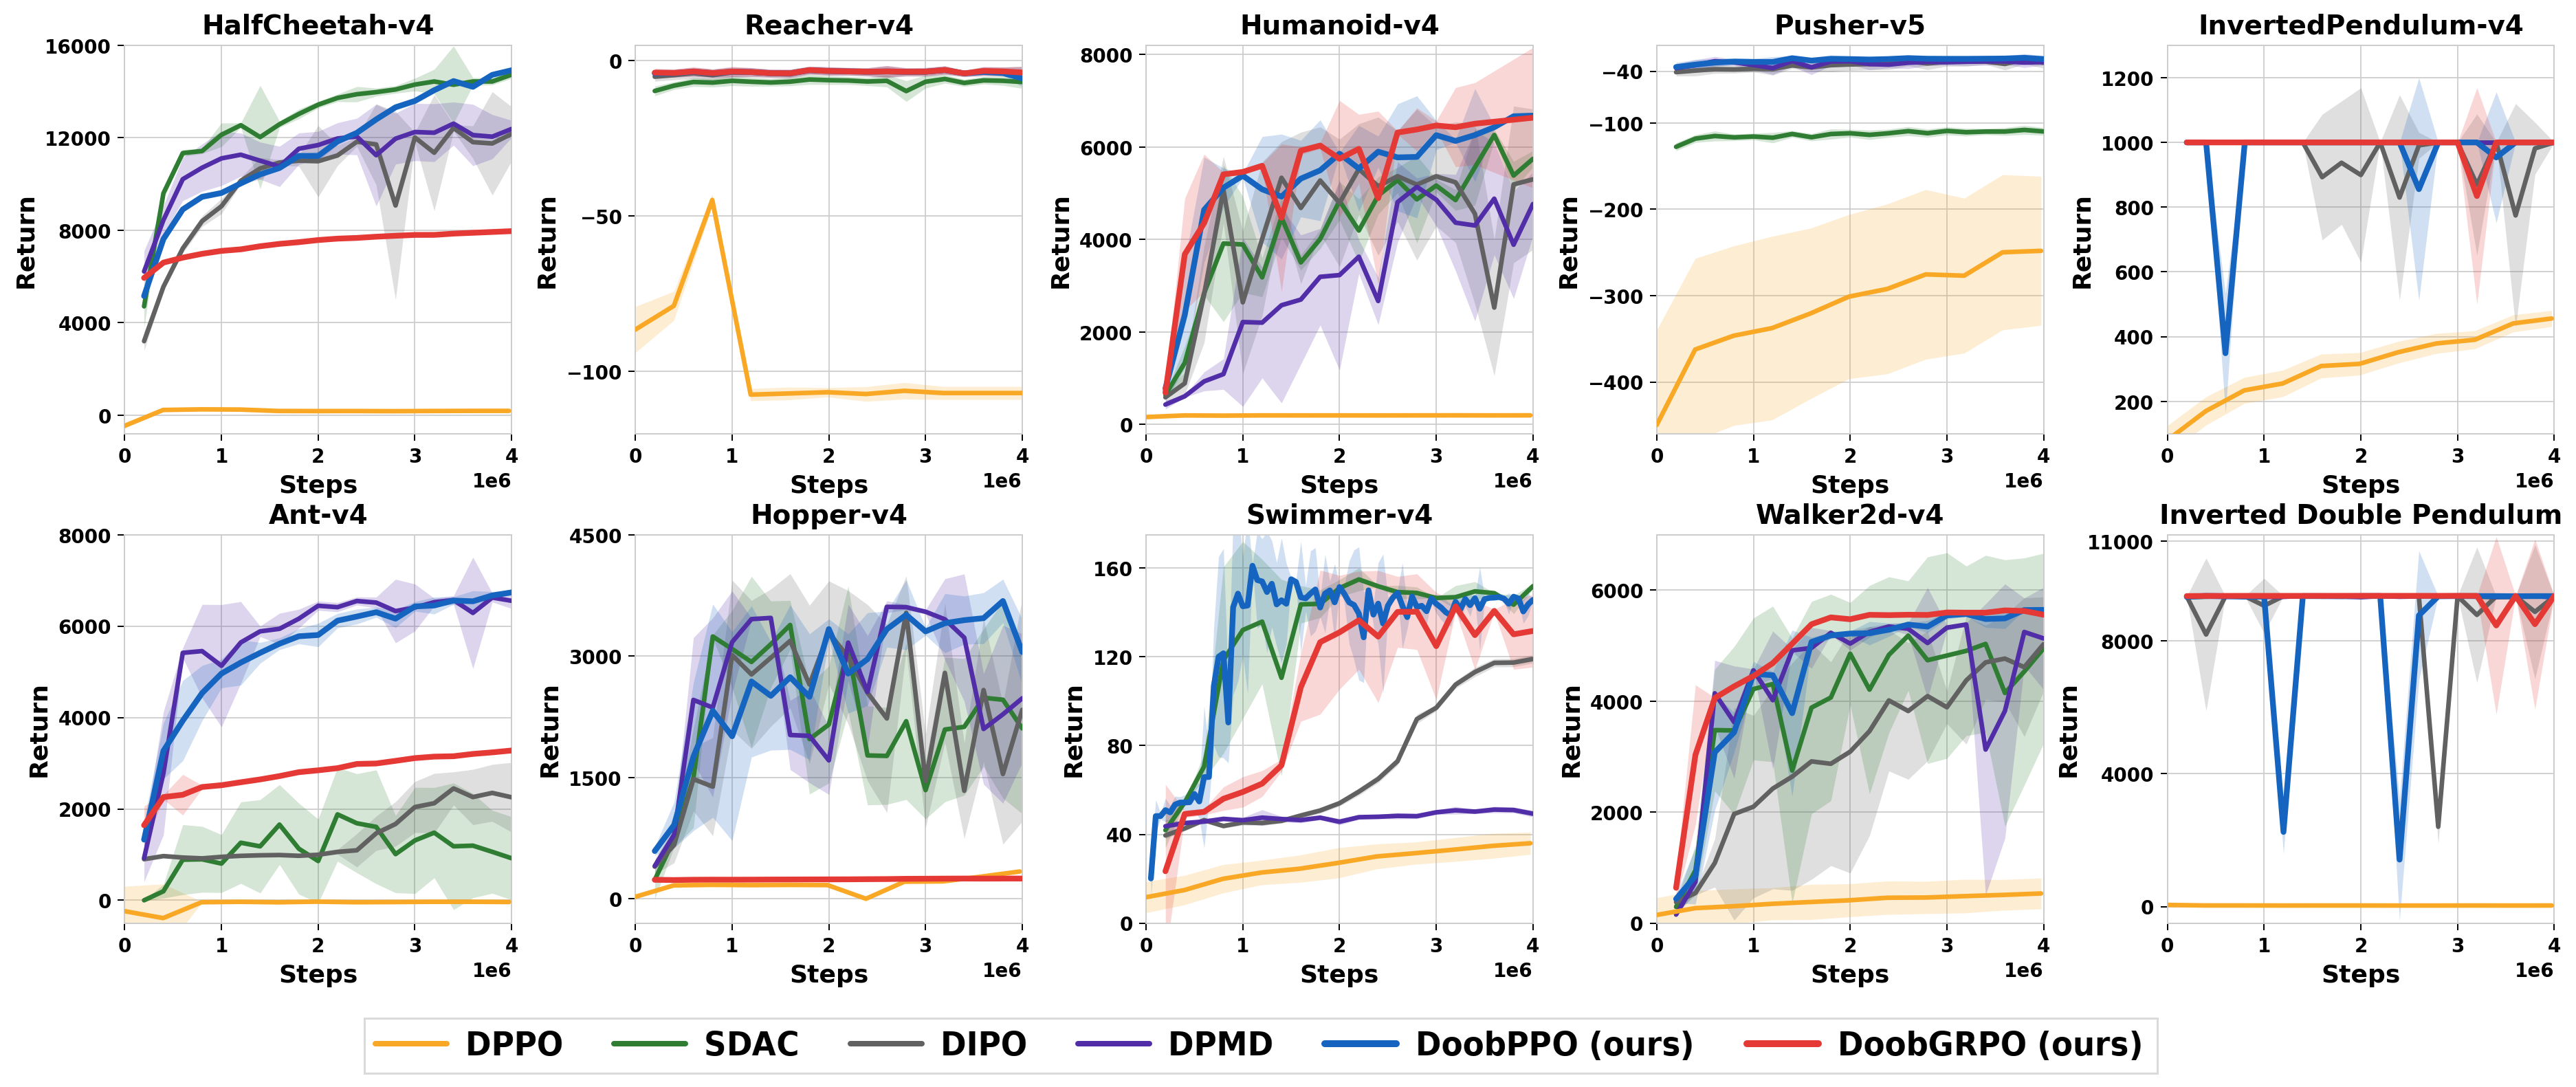
\includegraphics[width=1\linewidth]{mujoco10_4m_doob_grid.png}
    \caption{\small Learning curves on 10 MuJoCo continuous-control tasks, evaluated every 200k environment steps. Curves show mean undiscounted return over 3 training seeds, with shaded regions indicating one standard deviation. We compare DoobPO against strong diffusion-policy baselines DPPO, SDAC, DIPO, and DPMD.}
    \label{fig:mujoco10_dp}
\end{figure}

This section presents the experimental results.
We evaluate DoobPO on OpenAI Gym MuJoCo continuous-control benchmarks and on Robomimic manipulation tasks.
We describe the experimental setup in \cref{sec:exp_setup}.
We then report the results of RL fine-tuning diffusion and flow policies with DoobPO in \cref{sec:diffusion_exp} and \cref{sec:flow_exp}, and the Robomimic results in \cref{sec:robomimic_exp}.

\subsection{Experimental Setup}
\label{sec:exp_setup}

\textbf{Environments: OpenAI Gym MuJoCo.}
We evaluate our method on 10 OpenAI Gym MuJoCo continuous-control tasks covering locomotion, manipulation, and stabilization.
All diffusion-policy methods are trained from scratch for $4$M environment steps, while all flow-policy methods are trained from scratch for $5$M environment steps, under the same interaction budget within each setting.

\paragraph{Evaluation Metric.}
We use episode return as the evaluation metric, where higher return indicates better control performance.
During training, the policy is evaluated periodically, and at each evaluation point we report the mean return and its standard deviation over 3 random seeds.

\subsection{Diffusion Policy Comparison}
\label{sec:diffusion_exp}

\paragraph{Baselines.}
We compare DoobPO against recent diffusion-policy RL baselines, including DIPO \cite{yang2023policyrepresentationdiffusionprobability}, DPPO \cite{ren2024diffusion}, DPMD \cite{ma2025efficient}, DACER \cite{wang2024diffusionactorcriticentropyregulator}, and SDAC \cite{ma2025efficient}, as well as PPO \cite{schulman2017proximal}, TRPO \cite{schulman2015trust}, and SAC \cite{haarnoja2018soft}.
Please see \cref{sec:related_works} for details.

\begin{table*}[t]
\centering
\small
\setlength{\tabcolsep}{3.5pt}
\renewcommand{\arraystretch}{0.95}
\caption{\small Diffusion Policy Performance on MuJoCo environments
(mean $\pm$ std over 3 random seeds).
The best results are in bold and the second-best results are underlined.}
\label{tab:mujoco_grouped}
\begin{adjustbox}{max width=\textwidth}
\resizebox{0.9\linewidth}{!}{%
\begin{tabular}{llccccc}
\toprule
& Method
& HalfCheetah
& Reacher
& Humanoid
& Pusher
& InvertedPendulum \\
\midrule

\multirow{3}{*}{\textbf{Classic Model-Free RL}}
& PPO
& 1696 $\pm$ 223
& -3.63 $\pm$ 1.54
& 492 $\pm$ 113
& -25.28 $\pm$ 2.73
& \textbf{1000 $\pm$ 0} \\

& TRPO
& 2941 $\pm$ 417
& -3.83 $\pm$ 1.89
& 440 $\pm$ 82
& -31.84 $\pm$ 6.32
& \textbf{1000 $\pm$ 0} \\

& SAC
& 14422 $\pm$ 20
& -3.03 $\pm$ 1.21
& 5866 $\pm$ 16
& -23.96 $\pm$ 3.47
& \textbf{1000 $\pm$ 0} \\

\midrule

\multirow{7}{*}{\textbf{Diffusion Policy RL}}
& DIPO
& 12169 $\pm$ 1172
& -3.09 $\pm$ 1.36
& 5523 $\pm$ 980
& -27.85 $\pm$ 2.08
& \textbf{1000 $\pm$ 0} \\

& DPPO
& 248 $\pm$ 28
& -11.82 $\pm$ 1.28
& 195 $\pm$ 17
& -248.11 $\pm$ 86.32
& 456 $\pm$ 25 \\

& DPMD
& 12612 $\pm$ 932
& -2.97 $\pm$ 1.34
& 5138 $\pm$ 191
& -28.22 $\pm$ 6.06
& \textbf{1000 $\pm$ 0} \\

& DACER
& 14037 $\pm$ 370
& -2.973 $\pm$ 0.004
& 6460 $\pm$ 494
& -24.59 $\pm$ 0.37
& \textbf{1000 $\pm$ 0} \\

& SDAC
& \underline{14731 $\pm$ 166}
& -5.83 $\pm$ 1.36
& 6173 $\pm$ 1592
& -108 $\pm$ 5.23
& \textbf{1000 $\pm$ 0} \\

& \textbf{DoobPPO (ours)}
& \textbf{14921 $\pm$ 39}
& \underline{-2.96 $\pm$ 0.02}
& \textbf{6679 $\pm$ 63}
& \underline{-23.67 $\pm$ 3.16}
& \textbf{1000 $\pm$ 0} \\

& \textbf{DoobGRPO (ours)}
& 7800 $\pm$ 271
& \textbf{-2.95 $\pm$ 1.35}
& \underline{6634 $\pm$ 1517}
& \textbf{-23.62 $\pm$ 4.35}
& \textbf{1000 $\pm$ 0} \\

\midrule

& Method
& Ant
& Hopper
& Swimmer
& Walker2d
& Inverted2Pendulum \\
\midrule

\multirow{3}{*}{\textbf{Classic Model-Free RL}}
& PPO
& 1973 $\pm$ 67
& 1280 $\pm$ 197
& 121 $\pm$ 1.7
& 1242 $\pm$ 693
& \textbf{9360 $\pm$ 0} \\

& TRPO
& 3294 $\pm$ 76
& 3626 $\pm$ 9
& 42 $\pm$ 1.7
& 2765 $\pm$ 689
& 9188 $\pm$ 420 \\

& SAC
& 6534 $\pm$ 123
& 3533 $\pm$ 19
& 139 $\pm$ 1.1
& \textbf{6882 $\pm$ 60}
& \textbf{9360 $\pm$ 0} \\

\midrule

\multirow{7}{*}{\textbf{Diffusion Policy RL}}
& DIPO
& 2448 $\pm$ 361
& 3535 $\pm$ 456
& 119 $\pm$ 1.8
& 5028 $\pm$ 849
& 9351 $\pm$ 0.5 \\

& DPPO
& -29.9 $\pm$ 1.7
& 338 $\pm$ 5.1
& 36 $\pm$ 5
& 535 $\pm$ 278
& 32.7 $\pm$ 3.8 \\

& DPMD
& 6358 $\pm$ 276
& 3608 $\pm$ 73
& 51.1 $\pm$ 1.4
& 5381 $\pm$ 26
& 9355 $\pm$ 3.7 \\

& DACER
& \textbf{7137 $\pm$ 137}
& \textbf{3774 $\pm$ 106}
& 145.1 $\pm$ 5.4
& 5384 $\pm$ 1174
& 4096 $\pm$ 4778 \\

& SDAC
& 1880 $\pm$ 1025
& 3384 $\pm$ 303
& \underline{154 $\pm$ 5.1}
& 5181 $\pm$ 986
& 9353 $\pm$ 0.3 \\

& \textbf{DoobPPO (ours)}
& \underline{6738 $\pm$ 53}
& \underline{3681 $\pm$ 269}
& \textbf{161 $\pm$ 0.7}
& \underline{5642 $\pm$ 13}
& \underline{9356 $\pm$ 3} \\

& \textbf{DoobGRPO (ours)}
& 3278 $\pm$ 40
& 251 $\pm$ 1.4
& 142 $\pm$ 2.4
& 5636 $\pm$ 10
& \textbf{9360 $\pm$ 0} \\

\bottomrule
\end{tabular}}
\end{adjustbox}
\end{table*}

\paragraph{Diffusion Policy Results.}
Table~\ref{tab:mujoco_grouped} and Figure~1 report the
diffusion-policy results.
Overall, DoobPO achieves the highest mean returns among
diffusion-policy RL methods on 8 out of 10 MuJoCo tasks,
including ties.
DoobPPO obtains the best results on HalfCheetah, Humanoid,
and Swimmer, while DoobGRPO performs best on Reacher
and Pusher.
Both variants achieve competitive performance on the
remaining tasks, while DACER obtains the highest returns
on Ant and Hopper.

Compared with DIPO, DoobPPO improves performance by
22.6\% on HalfCheetah, 20.9\% on Humanoid,
175.2\% on Ant, and 12.2\% on Walker2d.
It also improves over DPMD by 18.3\%, 30.0\%,
6.0\%, and 4.9\% on the same tasks, respectively.
Against SDAC, DoobPPO achieves gains of 8.2\%
on Humanoid, 8.8\% on Hopper, and 8.9\%
on Walker2d.
The strong performance of DoobGRPO on Reacher and
Pusher further demonstrates that the framework is not
limited to a single PPO-style instantiation.
Together, these results establish DoobPO as a competitive
and flexible framework for diffusion-policy RL.

\subsection{Flow Policy Comparison}
\label{sec:flow_exp}

\begin{figure}[!t]
    \centering
    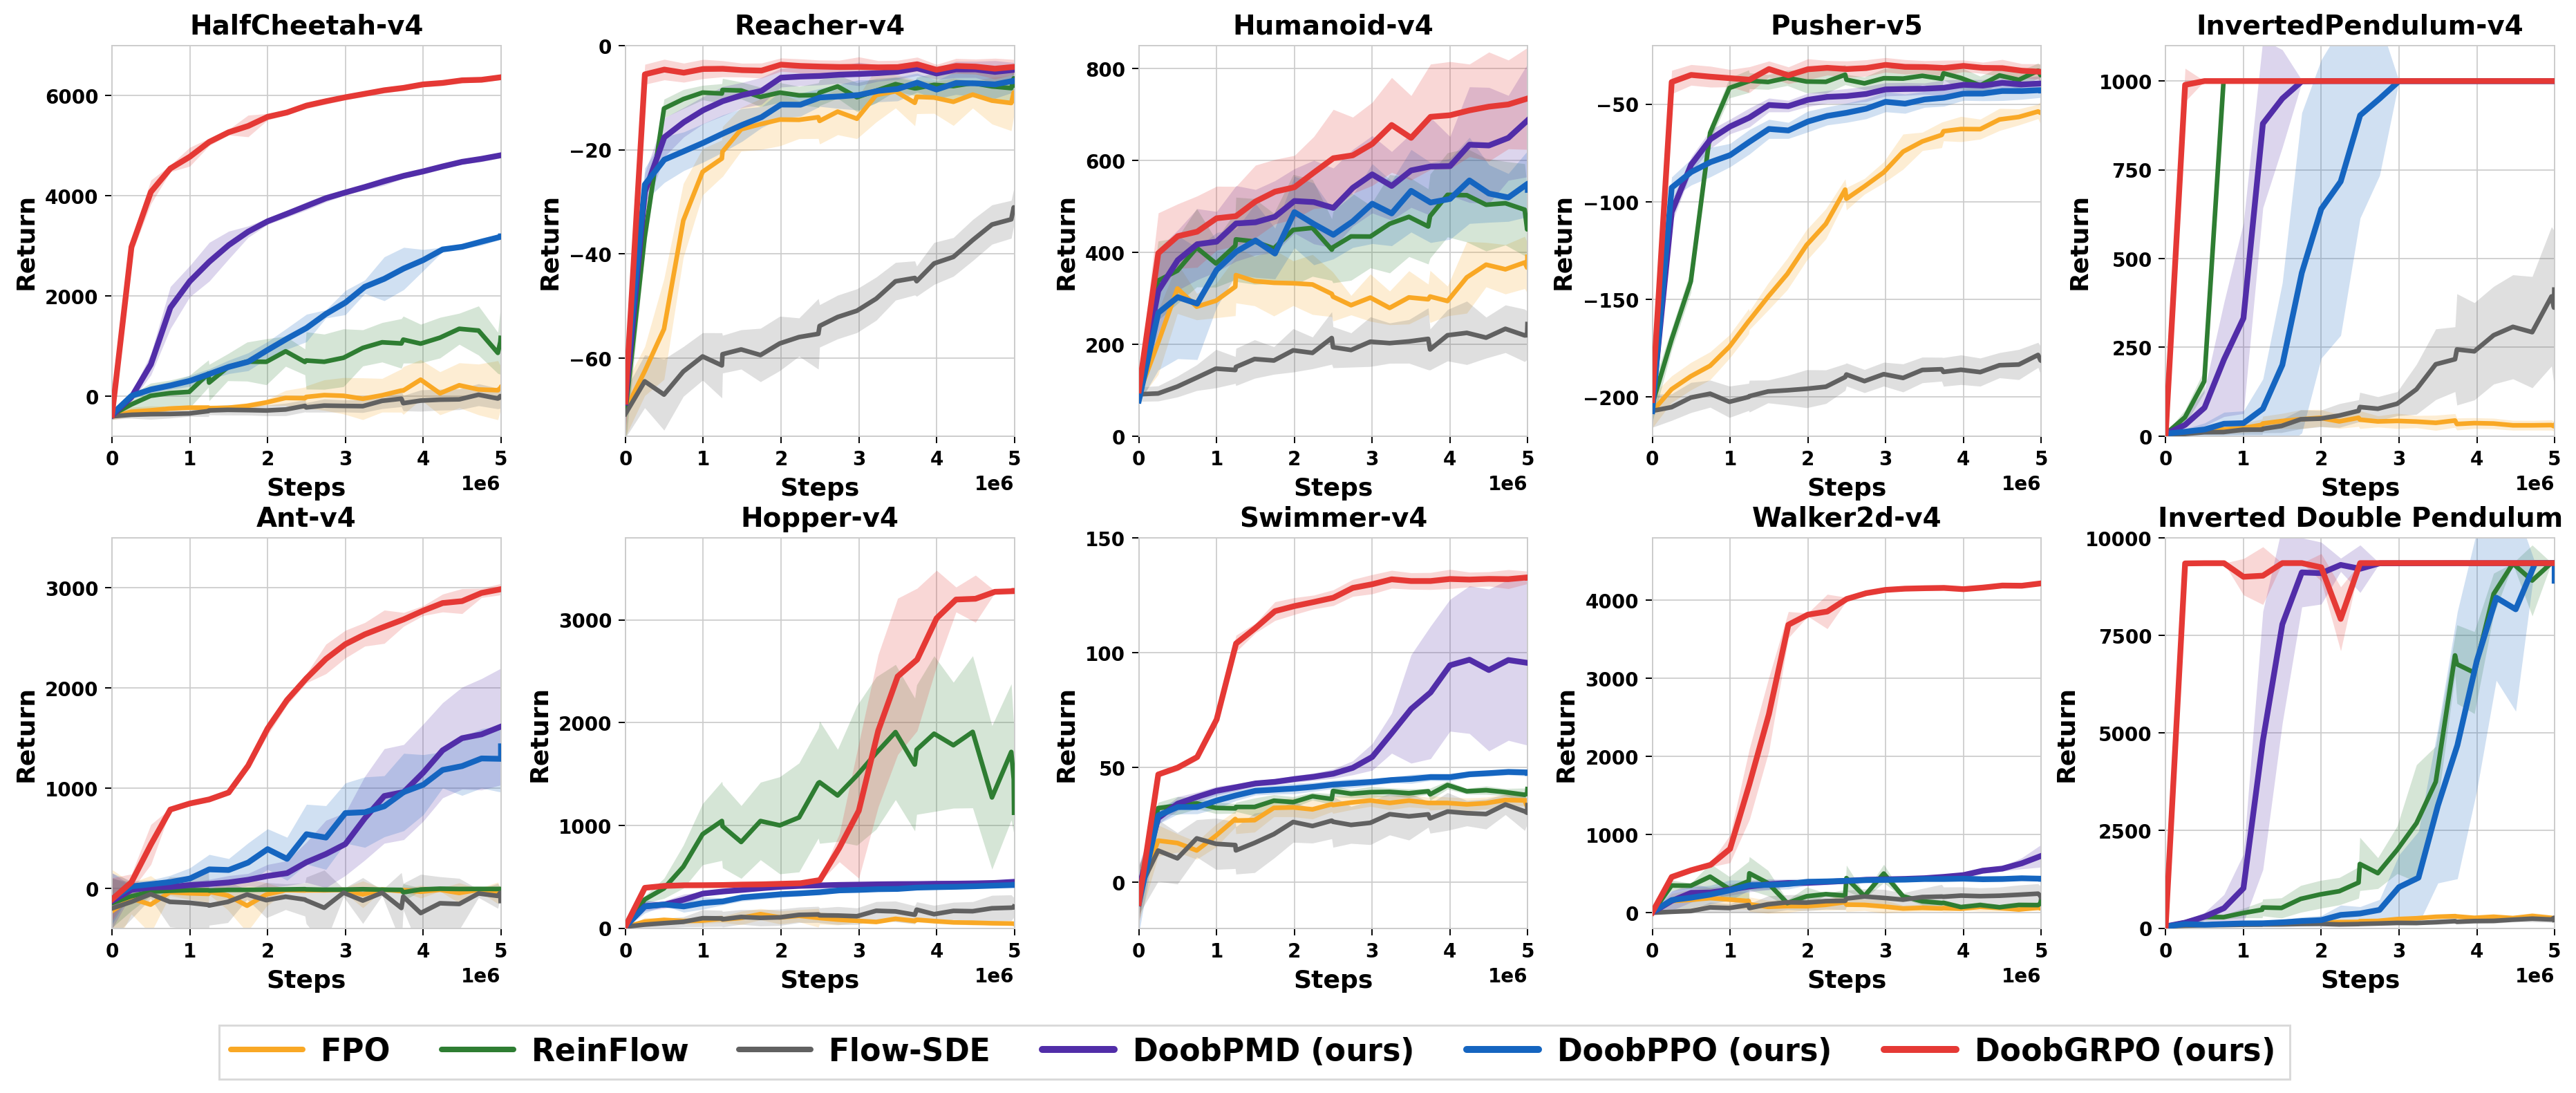
\includegraphics[width=1\linewidth]{mujoco10_flow_doob_grid.png}
    \caption{\small Learning curves on 10 MuJoCo continuous-control tasks, evaluated every 250k environment steps. Curves show mean undiscounted return over 3 training seeds, with shaded regions indicating one standard deviation. We compare DoobPO variants against flow-policy baselines FPO, ReinFlow, and Flow-SDE.}
    \label{fig:mujoco10_flow}
\end{figure}

\paragraph{Baselines.}
We compare DoobPO against three representative baselines for RL fine-tuning of flow policies: FPO \cite{mcallister2025flow}, ReinFlow \cite{zhang2025reinflow}, and Flow-SDE \cite{chen2025pirl}.
Please see \cref{sec:related_works} for more details.

\begin{table*}[t]
\centering
\small
\setlength{\tabcolsep}{3.5pt}
\renewcommand{\arraystretch}{0.95}
\caption{\small Flow Policy Performance on MuJoCo environments (mean $\pm$ std over 3 random seeds).}
\label{tab:mujoco_flow_grouped}
\begin{adjustbox}{max width=\textwidth}
\begin{tabular}{llccccc}
\toprule
& Method
& HalfCheetah
& Reacher
& Humanoid
& Pusher
& InvertedPendulum \\
\midrule

\multirow{6}{*}{\textbf{Flow Policy RL}}
& FPO
& 327 $\pm$ 399
& -8.79 $\pm$ 3.20
& 390 $\pm$ 110
& -53.77 $\pm$ 3.69
& 52 $\pm$ 24 \\

& ReinFlow
& 1344 $\pm$ 310
& -6.30 $\pm$ 2.83
& 525 $\pm$ 92
& \underline{-32.85 $\pm$ 3.81}
& \textbf{1000 $\pm$ 0} \\

& Flow-SDE
& 27 $\pm$ 219
& -31.08 $\pm$ 3.53
& 244 $\pm$ 60
& -178.42 $\pm$ 6.41
& 413 $\pm$ 238 \\

& \textbf{DoobPMD (ours)}
& \underline{4810 $\pm$ 53}
& \underline{-4.35 $\pm$ 1.40}
& \underline{688 $\pm$ 123}
& -39.10 $\pm$ 4.08
& \textbf{1000 $\pm$ 0} \\

& \textbf{DoobPPO (ours)}
& 3190 $\pm$ 60
& -6.73 $\pm$ 2.16
& 556 $\pm$ 94
& -42.81 $\pm$ 3.75
& \textbf{1000 $\pm$ 0} \\

& \textbf{DoobGRPO (ours)}
& \textbf{6368 $\pm$ 51}
& \textbf{-3.60 $\pm$ 1.37}
& \textbf{735 $\pm$ 111}
& \textbf{-29.90 $\pm$ 3.74}
& \textbf{1000 $\pm$ 0} \\

\midrule

& Method
& Ant
& Hopper
& Swimmer
& Walker2d
& Inverted2Pendulum \\
\midrule

\multirow{6}{*}{\textbf{Flow Policy RL}}
& FPO
& -13 $\pm$ 13
& 137 $\pm$ 55
& 35.8 $\pm$ 2.51
& 186 $\pm$ 140
& 314 $\pm$ 84 \\

& ReinFlow
& -5 $\pm$ 12
& \underline{1911 $\pm$ 740}
& 42.3 $\pm$ 1.77
& 503 $\pm$ 213
& \textbf{9358 $\pm$ 1} \\

& Flow-SDE
& -45 $\pm$ 41
& 210 $\pm$ 100
& 33.9 $\pm$ 4.44
& 243 $\pm$ 128
& 268 $\pm$ 68 \\

& \textbf{DoobPMD (ours)}
& \underline{1614 $\pm$ 583}
& 452 $\pm$ 4
& \underline{96.9 $\pm$ 32.13}
& \underline{726 $\pm$ 144}
& 9348 $\pm$ 0 \\

& \textbf{DoobPPO (ours)}
& 1417 $\pm$ 203
& 423 $\pm$ 10
& 48.0 $\pm$ 1.30
& 440 $\pm$ 16
& \underline{9350 $\pm$ 1} \\

& \textbf{DoobGRPO (ours)}
& \textbf{2986 $\pm$ 56}
& \textbf{3282 $\pm$ 7}
& \textbf{132.7 $\pm$ 2.71}
& \textbf{4215 $\pm$ 13}
& \underline{9350 $\pm$ 1} \\

\bottomrule
\end{tabular}
\end{adjustbox}
\end{table*}

\paragraph{Flow Policy Results.}
Table~\ref{tab:mujoco_flow_grouped} and Figure~\ref{fig:mujoco10_flow} report the flow-policy results.
Overall, DoobGRPO achieves the strongest performance across the MuJoCo benchmark under the same 5M-step training budget, obtaining the best results on 9 out of 10 tasks (including ties).
Compared with prior flow-policy RL baselines, DoobGRPO gives large gains on key locomotion tasks.
For example, it improves over the strongest baseline ReinFlow by \textbf{373.8\%} on \texttt{HalfCheetah}, \textbf{71.7\%} on \texttt{Hopper}, \textbf{213.7\%} on \texttt{Swimmer}, and \textbf{738.0\%} on \texttt{Walker2d}.
On the manipulation tasks, DoobGRPO also achieves the best performance on \texttt{Reacher} and \texttt{Pusher}, improving over ReinFlow by \textbf{42.9\%} and \textbf{9.0\%}.
DoobPMD serves as a strong second-best on several tasks, including \texttt{HalfCheetah}, \texttt{Reacher}, and \texttt{Humanoid}.
This further demonstrates the generality of the DoobPO framework across different policy-gradient methods.
These results show that DoobPO provides a useful RL framework for flow policies.

\subsection{Robomimic Manipulation}
\label{sec:robomimic_exp}

\paragraph{Setup.}
To evaluate DoobPO beyond MuJoCo continuous control, we test it on the \texttt{Can} and \texttt{Square} manipulation tasks from Robomimic \cite{mandlekar2021matters}.
Both tasks use low-dimensional state observations, sparse binary success rewards, and an action-chunk horizon of 4.
The maximum episode lengths are 300 primitive steps for \texttt{Can} and 400 for \texttt{Square}.
We follow the official Robomimic evaluation protocol with 50 parallel environments.
An episode is successful if the binary task-completion reward is achieved at least once, and the success rate is computed over all completed evaluation episodes.
We compare DoobPPO with DPPO \cite{ren2024diffusion}.
Both methods are initialized from the same pretrained diffusion behavior-cloning policy and trained for 151 iterations on \texttt{Can} and 200 iterations on \texttt{Square}, and results are averaged over 3 random seeds.
The DoobPPO hyperparameters are listed in \cref{tab:hyperparameters_robomimic}.

\paragraph{Results.}
DoobPPO matches or slightly improves upon DPPO on both tasks, reaching success rates of 99.46\% versus 99.23\% on \texttt{Can} and 99.78\% versus 99.59\% on \texttt{Square}.
Since both tasks are close to saturation, the main takeaway is not a large performance gap but that DoobPO extends to sparse-reward manipulation settings.

\subsection{Implementation Details and Ablation Studies}

Additional implementation details are provided in \cref{sec:implementation}, including computational resources, training hyperparameters, and other reproducibility details.
We also include ablation studies in \cref{sec:ablation} to examine the effect of the ratio network size and the number of sampling steps.


\section{Discussion and Conclusion}
\label{sec:conclusion}In this work, we introduce \textbf{Doob Policy Optimization (DoobPO)}, a unified framework for RL fine-tuning of diffusion and flow policies.
The framework supports a broad family of policy updates and avoids exact action-likelihood evaluation by separating policy improvement from generative policy learning.
Theoretically, we justify DoobPO from two directions.
First, we characterize the ratio-tilted diffusion process through Doob's $h$-transform
(\cref{lem:algo_correctness}).
We then show that, for each fixed state, the gradient of the conditional drift matching objective is proportional to that of the ideal objective for both diffusion and flow policies
(\cref{thm:grad_equi_diff,thm:grad_equi_fm}).
Second, under the stated assumptions, the population minimizer of conditional drift matching induces a diffusion process that solves the corresponding endpoint-constrained stochastic optimal control problem
(\cref{prop:cdm_solves_soc}).
The resulting process is the minimum-energy modification of the reference diffusion that realizes the prescribed tilted endpoint marginals.
This provides a control-theoretic interpretation of how the desired policy update is transferred into generative dynamics.
Experimentally, we evaluate DoobPO on MuJoCo benchmarks with both diffusion and flow policies and observe superior overall performance against strong baselines
(\cref{sec:diffusion_exp,sec:flow_exp}).

More broadly, DoobPO provides a common interface between policy optimization and generative model training.
Policy updates with analytic ratios and updates represented by learned ratio models are accommodated within the same conditional drift matching framework
(\cref{sec:unified_framework}).
This separates the choice of the policy update rule from the choice of the generative policy class.
Nevertheless, our study mainly focuses on continuous generation, and the empirical evaluation is limited to MuJoCo continuous-control benchmarks and Robomimic manipulation tasks.
The theoretical results characterize population objectives under the stated assumptions.
An important direction for future work is to quantify how ratio estimation error and approximate drift matching affect the realized policy update.
We also plan to extend the framework to discrete generation and evaluate its applicability to more complex policy learning settings.


\clearpage


% \section*{Acknowledgments}
% Han Liu is partially supported by NIH R01LM1372201, NSF
AST-2421845, Simons Foundation
MPS-AI-00010513, AbbVie , Dolby and Chan Zuckerberg Biohub Chicago Spoke Award.
This research was supported in part through the computational resources and staff contributions provided for the Quest high performance computing facility at Northwestern University which is jointly supported by the Office of the Provost, the Office for Research, and Northwestern University Information Technology.
The content is solely the responsibility of the authors and does not necessarily represent the official
views of the funding agencies.









% \clearpage
\bibliographystyle{unsrtnat}
% \bibliographystyle{plainnat}
% \bibliographystyle{apalike}
% \bibliographystyle{alpha}
\bibliography{refs}



\newpage  % start from a new page
\normalsize
% Reset section title spacing to defaults
\titlespacing*{\section}{0pt}{*1}{*1}
\titlespacing*{\subsection}{0pt}{*1.25}{*1.25}
\titlespacing*{\subsubsection}{0pt}{*1.5}{*1.5}
\setlist[itemize]{leftmargin=1em}
\setlist[enumerate]{leftmargin=1.4em}


% Reset equation spacing to defaults
\setlength{\abovedisplayskip}{10pt}
\setlength{\abovedisplayshortskip}{10pt}
\setlength{\belowdisplayskip}{10pt}
\setlength{\belowdisplayshortskip}{10pt}



% {
% \setlength{\parskip}{0em}
% \setcounter{tocdepth}{2}
% \tableofcontents
% }
% \setcounter{footnote}{0}

% \clearpage

\appendix
\label{sec:append}
% \part*{Appendix}
%\begin{center}
%	{\LARGE \textbf{Appendix}}
%\end{center}
{
\setlength{\parskip}{-0em}
\startcontents[sections]
\printcontents[sections]{ }{1}{}
}

% \clearpage
% \section*{NeurIPS Paper Checklist}

%%% BEGIN INSTRUCTIONS %%%
% The checklist is designed to encourage best practices for responsible machine learning research, addressing issues of reproducibility, transparency, research ethics, and societal impact. Do not remove the checklist: {\bf The papers not including the checklist will be desk rejected.} The checklist should follow the references and follow the (optional) supplemental material.  The checklist does NOT count towards the page
% limit. 

% Please read the checklist guidelines carefully for information on how to answer these questions. For each question in the checklist:
% \begin{itemize}
%     \item You should answer \answerYes{}, \answerNo{}, or \answerNA{}.
%     \item \answerNA{} means either that the question is Not Applicable for that particular paper or the relevant information is Not Available.
%     \item Please provide a short (1--2 sentence) justification right after your answer (even for \answerNA). 
%    % \item {\bf The papers not including the checklist will be desk rejected.}
% \end{itemize}

% {\bf The checklist answers are an integral part of your paper submission.} They are visible to the reviewers, area chairs, senior area chairs, and ethics reviewers. You will also be asked to include it (after eventual revisions) with the final version of your paper, and its final version will be published with the paper.

% The reviewers of your paper will be asked to use the checklist as one of the factors in their evaluation. While \answerYes{} is generally preferable to \answerNo{}, it is perfectly acceptable to answer \answerNo{} provided a proper justification is given (e.g., error bars are not reported because it would be too computationally expensive'' or ``we were unable to find the license for the dataset we used''). In general, answering \answerNo{} or \answerNA{} is not grounds for rejection. While the questions are phrased in a binary way, we acknowledge that the true answer is often more nuanced, so please just use your best judgment and write a justification to elaborate. All supporting evidence can appear either in the main paper or the supplemental material, provided in appendix. If you answer \answerYes{} to a question, in the justification please point to the section(s) where related material for the question can be found.

% IMPORTANT, please:
% \begin{itemize}
%     \item {\bf Delete this instruction block, but keep the section heading ``NeurIPS Paper Checklist"},
%     \item  {\bf Keep the checklist subsection headings, questions/answers and guidelines below.}
%     \item {\bf Do not modify the questions and only use the provided macros for your answers}.
% \end{itemize} 
 

%%% END INSTRUCTIONS %%%


\begin{enumerate}

\item {\bf Claims}
    \item[] Question: Do the main claims made in the abstract and introduction accurately reflect the paper's contributions and scope?
    \item[] Answer: \answerYes{} % Replace by \answerYes{}, \answerNo{}, or \answerNA{}.
    \item[] Justification: All main claims are stated in the abstract, introduction, and theorem statements.
    \item[] Guidelines:
    \begin{itemize}
        \item The answer \answerNA{} means that the abstract and introduction do not include the claims made in the paper.
        \item The abstract and/or introduction should clearly state the claims made, including the contributions made in the paper and important assumptions and limitations. A \answerNo{} or \answerNA{} answer to this question will not be perceived well by the reviewers. 
        \item The claims made should match theoretical and experimental results, and reflect how much the results can be expected to generalize to other settings. 
        \item It is fine to include aspirational goals as motivation as long as it is clear that these goals are not attained by the paper. 
    \end{itemize}

\item {\bf Limitations}
    \item[] Question: Does the paper discuss the limitations of the work performed by the authors?
    \item[] Answer: \answerYes{} % Replace by \answerYes{}, \answerNo{}, or \answerNA{}.
    \item[] Justification:
    We discuss limitations in \cref{sec:conclusion}.
    We discuss the method now only support continuous generation.
    We may extend this to discrete setting.
    \item[] Guidelines:
    \begin{itemize}
        \item The answer \answerNA{} means that the paper has no limitation while the answer \answerNo{} means that the paper has limitations, but those are not discussed in the paper. 
        \item The authors are encouraged to create a separate ``Limitations'' section in their paper.
        \item The paper should point out any strong assumptions and how robust the results are to violations of these assumptions (e.g., independence assumptions, noiseless settings, model well-specification, asymptotic approximations only holding locally). The authors should reflect on how these assumptions might be violated in practice and what the implications would be.
        \item The authors should reflect on the scope of the claims made, e.g., if the approach was only tested on a few datasets or with a few runs. In general, empirical results often depend on implicit assumptions, which should be articulated.
        \item The authors should reflect on the factors that influence the performance of the approach. For example, a facial recognition algorithm may perform poorly when image resolution is low or images are taken in low lighting. Or a speech-to-text system might not be used reliably to provide closed captions for online lectures because it fails to handle technical jargon.
        \item The authors should discuss the computational efficiency of the proposed algorithms and how they scale with dataset size.
        \item If applicable, the authors should discuss possible limitations of their approach to address problems of privacy and fairness.
        \item While the authors might fear that complete honesty about limitations might be used by reviewers as grounds for rejection, a worse outcome might be that reviewers discover limitations that aren't acknowledged in the paper. The authors should use their best judgment and recognize that individual actions in favor of transparency play an important role in developing norms that preserve the integrity of the community. Reviewers will be specifically instructed to not penalize honesty concerning limitations.
    \end{itemize}

\item {\bf Theory assumptions and proofs}
    \item[] Question: For each theoretical result, does the paper provide the full set of assumptions and a complete (and correct) proof?
    \item[] Answer: \answerYes{} % Replace by \answerYes{}, \answerNo{}, or \answerNA{}.
    \item[] Justification:
    All assumptions are stated in the main text, and complete proofs are provided in the appendix.
    \item[] Guidelines:
    \begin{itemize}
        \item The answer \answerNA{} means that the paper does not include theoretical results. 
        \item All the theorems, formulas, and proofs in the paper should be numbered and cross-referenced.
        \item All assumptions should be clearly stated or referenced in the statement of any theorems.
        \item The proofs can either appear in the main paper or the supplemental material, but if they appear in the supplemental material, the authors are encouraged to provide a short proof sketch to provide intuition. 
        \item Inversely, any informal proof provided in the core of the paper should be complemented by formal proofs provided in appendix or supplemental material.
        \item Theorems and Lemmas that the proof relies upon should be properly referenced. 
    \end{itemize}

    \item {\bf Experimental result reproducibility}
    \item[] Question: Does the paper fully disclose all the information needed to reproduce the main experimental results of the paper to the extent that it affects the main claims and/or conclusions of the paper (regardless of whether the code and data are provided or not)?
    \item[] Answer: \answerYes{} % Replace by \answerYes{}, \answerNo{}, or \answerNA{}.
    \item[] Justification: We fully disclose all the information needed.
    \item[] Guidelines:
    \begin{itemize}
        \item The answer \answerNA{} means that the paper does not include experiments.
        \item If the paper includes experiments, a \answerNo{} answer to this question will not be perceived well by the reviewers: Making the paper reproducible is important, regardless of whether the code and data are provided or not.
        \item If the contribution is a dataset and\slash or model, the authors should describe the steps taken to make their results reproducible or verifiable. 
        \item Depending on the contribution, reproducibility can be accomplished in various ways. For example, if the contribution is a novel architecture, describing the architecture fully might suffice, or if the contribution is a specific model and empirical evaluation, it may be necessary to either make it possible for others to replicate the model with the same dataset, or provide access to the model. In general. releasing code and data is often one good way to accomplish this, but reproducibility can also be provided via detailed instructions for how to replicate the results, access to a hosted model (e.g., in the case of a large language model), releasing of a model checkpoint, or other means that are appropriate to the research performed.
        \item While NeurIPS does not require releasing code, the conference does require all submissions to provide some reasonable avenue for reproducibility, which may depend on the nature of the contribution. For example
        \begin{enumerate}
            \item If the contribution is primarily a new algorithm, the paper should make it clear how to reproduce that algorithm.
            \item If the contribution is primarily a new model architecture, the paper should describe the architecture clearly and fully.
            \item If the contribution is a new model (e.g., a large language model), then there should either be a way to access this model for reproducing the results or a way to reproduce the model (e.g., with an open-source dataset or instructions for how to construct the dataset).
            \item We recognize that reproducibility may be tricky in some cases, in which case authors are welcome to describe the particular way they provide for reproducibility. In the case of closed-source models, it may be that access to the model is limited in some way (e.g., to registered users), but it should be possible for other researchers to have some path to reproducing or verifying the results.
        \end{enumerate}
    \end{itemize}


\item {\bf Open access to data and code}
    \item[] Question: Does the paper provide open access to the data and code, with sufficient instructions to faithfully reproduce the main experimental results, as described in supplemental material?
    \item[] Answer: \answerYes{} % Replace by \answerYes{}, \answerNo{}, or \answerNA{}.
    \item[] Justification: We show the details of experiments in the paper and we submit the code in the supplemental material.
    \item[] Guidelines:
    \begin{itemize}
        \item The answer \answerNA{} means that paper does not include experiments requiring code.
        \item Please see the NeurIPS code and data submission guidelines (\url{https://neurips.cc/public/guides/CodeSubmissionPolicy}) for more details.
        \item While we encourage the release of code and data, we understand that this might not be possible, so \answerNo{} is an acceptable answer. Papers cannot be rejected simply for not including code, unless this is central to the contribution (e.g., for a new open-source benchmark).
        \item The instructions should contain the exact command and environment needed to run to reproduce the results. See the NeurIPS code and data submission guidelines (\url{https://neurips.cc/public/guides/CodeSubmissionPolicy}) for more details.
        \item The authors should provide instructions on data access and preparation, including how to access the raw data, preprocessed data, intermediate data, and generated data, etc.
        \item The authors should provide scripts to reproduce all experimental results for the new proposed method and baselines. If only a subset of experiments are reproducible, they should state which ones are omitted from the script and why.
        \item At submission time, to preserve anonymity, the authors should release anonymized versions (if applicable).
        \item Providing as much information as possible in supplemental material (appended to the paper) is recommended, but including URLs to data and code is permitted.
    \end{itemize}


\item {\bf Experimental setting/details}
    \item[] Question: Does the paper specify all the training and test details (e.g., data splits, hyperparameters, how they were chosen, type of optimizer) necessary to understand the results?
    \item[] Answer: \answerYes{} % Replace by \answerYes{}, \answerNo{}, or \answerNA{}.
    \item[] Justification: The paper describes the model setting in \cref{sec:exp} and \cref{sec:implementation}.
    \item[] Guidelines:
    \begin{itemize}
        \item The answer \answerNA{} means that the paper does not include experiments.
        \item The experimental setting should be presented in the core of the paper to a level of detail that is necessary to appreciate the results and make sense of them.
        \item The full details can be provided either with the code, in appendix, or as supplemental material.
    \end{itemize}

\item {\bf Experiment statistical significance}
    \item[] Question: Does the paper report error bars suitably and correctly defined or other appropriate information about the statistical significance of the experiments?
    \item[] Answer: \answerYes{} % Replace by \answerYes{}, \answerNo{}, or \answerNA{}.
    \item[] Justification: We run the experiments with different seeds and report the mean and std. 
    \item[] Guidelines:
    \begin{itemize}
        \item The answer \answerNA{} means that the paper does not include experiments.
        \item The authors should answer \answerYes{} if the results are accompanied by error bars, confidence intervals, or statistical significance tests, at least for the experiments that support the main claims of the paper.
        \item The factors of variability that the error bars are capturing should be clearly stated (for example, train/test split, initialization, random drawing of some parameter, or overall run with given experimental conditions).
        \item The method for calculating the error bars should be explained (closed form formula, call to a library function, bootstrap, etc.)
        \item The assumptions made should be given (e.g., Normally distributed errors).
        \item It should be clear whether the error bar is the standard deviation or the standard error of the mean.
        \item It is OK to report 1-sigma error bars, but one should state it. The authors should preferably report a 2-sigma error bar than state that they have a 96\% CI, if the hypothesis of Normality of errors is not verified.
        \item For asymmetric distributions, the authors should be careful not to show in tables or figures symmetric error bars that would yield results that are out of range (e.g., negative error rates).
        \item If error bars are reported in tables or plots, the authors should explain in the text how they were calculated and reference the corresponding figures or tables in the text.
    \end{itemize}

\item {\bf Experiments compute resources}
    \item[] Question: For each experiment, does the paper provide sufficient information on the computer resources (type of compute workers, memory, time of execution) needed to reproduce the experiments?
    \item[] Answer: \answerYes{} % Replace by \answerYes{}, \answerNo{}, or \answerNA{}.
    \item[] Justification: We have mentioned all information about compute resources in \cref{sec:implementation}.
    \item[] Guidelines:
    \begin{itemize}
        \item The answer \answerNA{} means that the paper does not include experiments.
        \item The paper should indicate the type of compute workers CPU or GPU, internal cluster, or cloud provider, including relevant memory and storage.
        \item The paper should provide the amount of compute required for each of the individual experimental runs as well as estimate the total compute. 
        \item The paper should disclose whether the full research project required more compute than the experiments reported in the paper (e.g., preliminary or failed experiments that didn't make it into the paper). 
    \end{itemize}
    
\item {\bf Code of ethics}
    \item[] Question: Does the research conducted in the paper conform, in every respect, with the NeurIPS Code of Ethics \url{https://neurips.cc/public/EthicsGuidelines}?
    \item[] Answer: \answerYes{} % Replace by \answerYes{}, \answerNo{}, or \answerNA{}.
    \item[] Justification: We reviewed the NeurIPS Code of Ethics and believe the research conforms to it. 
    \item[] Guidelines:
    \begin{itemize}
        \item The answer \answerNA{} means that the authors have not reviewed the NeurIPS Code of Ethics.
        \item If the authors answer \answerNo, they should explain the special circumstances that require a deviation from the Code of Ethics.
        \item The authors should make sure to preserve anonymity (e.g., if there is a special consideration due to laws or regulations in their jurisdiction).
    \end{itemize}


\item {\bf Broader impacts}
    \item[] Question: Does the paper discuss both potential positive societal impacts and negative societal impacts of the work performed?
    \item[] Answer: \answerYes{} % Replace by \answerYes{}, \answerNo{}, or \answerNA{}.
    \item[] Justification: The paper includes an ethics statement and discusses the likely scope of the work.
    \item[] Guidelines:
    \begin{itemize}
        \item The answer \answerNA{} means that there is no societal impact of the work performed.
        \item If the authors answer \answerNA{} or \answerNo, they should explain why their work has no societal impact or why the paper does not address societal impact.
        \item Examples of negative societal impacts include potential malicious or unintended uses (e.g., disinformation, generating fake profiles, surveillance), fairness considerations (e.g., deployment of technologies that could make decisions that unfairly impact specific groups), privacy considerations, and security considerations.
        \item The conference expects that many papers will be foundational research and not tied to particular applications, let alone deployments. However, if there is a direct path to any negative applications, the authors should point it out. For example, it is legitimate to point out that an improvement in the quality of generative models could be used to generate Deepfakes for disinformation. On the other hand, it is not needed to point out that a generic algorithm for optimizing neural networks could enable people to train models that generate Deepfakes faster.
        \item The authors should consider possible harms that could arise when the technology is being used as intended and functioning correctly, harms that could arise when the technology is being used as intended but gives incorrect results, and harms following from (intentional or unintentional) misuse of the technology.
        \item If there are negative societal impacts, the authors could also discuss possible mitigation strategies (e.g., gated release of models, providing defenses in addition to attacks, mechanisms for monitoring misuse, mechanisms to monitor how a system learns from feedback over time, improving the efficiency and accessibility of ML).
    \end{itemize}
    
\item {\bf Safeguards}
    \item[] Question: Does the paper describe safeguards that have been put in place for responsible release of data or models that have a high risk for misuse (e.g., pre-trained language models, image generators, or scraped datasets)?
    \item[] Answer: \answerNA{} % Replace by \answerYes{}, \answerNo{}, or \answerNA{}.
    \item[] Justification: The paper does not release high-risk datasets, pre-trained models, or generative systems that require special safeguards. 
    \item[] Guidelines:
    \begin{itemize}
        \item The answer \answerNA{} means that the paper poses no such risks.
        \item Released models that have a high risk for misuse or dual-use should be released with necessary safeguards to allow for controlled use of the model, for example by requiring that users adhere to usage guidelines or restrictions to access the model or implementing safety filters. 
        \item Datasets that have been scraped from the Internet could pose safety risks. The authors should describe how they avoided releasing unsafe images.
        \item We recognize that providing effective safeguards is challenging, and many papers do not require this, but we encourage authors to take this into account and make a best faith effort.
    \end{itemize}

\item {\bf Licenses for existing assets}
    \item[] Question: Are the creators or original owners of assets (e.g., code, data, models), used in the paper, properly credited and are the license and terms of use explicitly mentioned and properly respected?
    \item[] Answer: \answerYes{} % Replace by \answerYes{}, \answerNo{}, or \answerNA{}.
    \item[] Justification:  All external assets used in this work are credited and used in accordance with their licenses. 
    \item[] Guidelines:
    \begin{itemize}
        \item The answer \answerNA{} means that the paper does not use existing assets.
        \item The authors should cite the original paper that produced the code package or dataset.
        \item The authors should state which version of the asset is used and, if possible, include a URL.
        \item The name of the license (e.g., CC-BY 4.0) should be included for each asset.
        \item For scraped data from a particular source (e.g., website), the copyright and terms of service of that source should be provided.
        \item If assets are released, the license, copyright information, and terms of use in the package should be provided. For popular datasets, \url{paperswithcode.com/datasets} has curated licenses for some datasets. Their licensing guide can help determine the license of a dataset.
        \item For existing datasets that are re-packaged, both the original license and the license of the derived asset (if it has changed) should be provided.
        \item If this information is not available online, the authors are encouraged to reach out to the asset's creators.
    \end{itemize}

\item {\bf New assets}
    \item[] Question: Are new assets introduced in the paper well documented and is the documentation provided alongside the assets?
    \item[] Answer: \answerYes{} % Replace by \answerYes{}, \answerNo{}, or \answerNA{}.
    \item[] Justification: All new assets introduced in the paper are well documented.
    \item[] Guidelines:
    \begin{itemize}
        \item The answer \answerNA{} means that the paper does not release new assets.
        \item Researchers should communicate the details of the dataset\slash code\slash model as part of their submissions via structured templates. This includes details about training, license, limitations, etc. 
        \item The paper should discuss whether and how consent was obtained from people whose asset is used.
        \item At submission time, remember to anonymize your assets (if applicable). You can either create an anonymized URL or include an anonymized zip file.
    \end{itemize}

\item {\bf Crowdsourcing and research with human subjects}
    \item[] Question: For crowdsourcing experiments and research with human subjects, does the paper include the full text of instructions given to participants and screenshots, if applicable, as well as details about compensation (if any)? 
    \item[] Answer: \answerNA{} % Replace by \answerYes{}, \answerNo{}, or \answerNA{}.
    \item[] Justification: The paper does not involve crowdsourcing experiments or research with human subjects.
    \item[] Guidelines:
    \begin{itemize}
        \item The answer \answerNA{} means that the paper does not involve crowdsourcing nor research with human subjects.
        \item Including this information in the supplemental material is fine, but if the main contribution of the paper involves human subjects, then as much detail as possible should be included in the main paper. 
        \item According to the NeurIPS Code of Ethics, workers involved in data collection, curation, or other labor should be paid at least the minimum wage in the country of the data collector. 
    \end{itemize}

\item {\bf Institutional review board (IRB) approvals or equivalent for research with human subjects}
    \item[] Question: Does the paper describe potential risks incurred by study participants, whether such risks were disclosed to the subjects, and whether Institutional Review Board (IRB) approvals (or an equivalent approval/review based on the requirements of your country or institution) were obtained?
    \item[] Answer: \answerNA{} % Replace by \answerYes{}, \answerNo{}, or \answerNA{}.
    \item[] Justification: The paper does not involve crowdsourcing or research with human subjects.
    \item[] Guidelines:
    \begin{itemize}
        \item The answer \answerNA{} means that the paper does not involve crowdsourcing nor research with human subjects.
        \item Depending on the country in which research is conducted, IRB approval (or equivalent) may be required for any human subjects research. If you obtained IRB approval, you should clearly state this in the paper. 
        \item We recognize that the procedures for this may vary significantly between institutions and locations, and we expect authors to adhere to the NeurIPS Code of Ethics and the guidelines for their institution. 
        \item For initial submissions, do not include any information that would break anonymity (if applicable), such as the institution conducting the review.
    \end{itemize}

\item {\bf Declaration of LLM usage}
    \item[] Question: Does the paper describe the usage of LLMs if it is an important, original, or non-standard component of the core methods in this research? Note that if the LLM is used only for writing, editing, or formatting purposes and does \emph{not} impact the core methodology, scientific rigor, or originality of the research, declaration is not required.
    %this research? 
    \item[] Answer: \answerNA{} % Replace by \answerYes{}, \answerNo{}, or \answerNA{}.
    \item[] Justification: We describe the usage of LLMs in the appendix.
    \item[] Guidelines:
    \begin{itemize}
        \item The answer \answerNA{} means that the core method development in this research does not involve LLMs as any important, original, or non-standard components.
        \item Please refer to our LLM policy in the NeurIPS handbook for what should or should not be described.
    \end{itemize}

\end{enumerate}


\clearpage
\part*{Appendix}
\appendix	
{
\setlength{\parskip}{0.3em}
\startcontents[sections]
\printcontents[sections]{ }{1}{}
}
% \clearpage
% \section*{Broader Impact}
% \input{boarder}
% \part*{Supplementary Material}
% %\begin{center}
% %	{\LARGE \textbf{Appendix}}
% %\end{center}
{
\setlength{\parskip}{-0em}
\startcontents[sections]
\printcontents[sections]{ }{1}{}
}
\clearpage

\section*{Impact Statement}
This work advances the methodological and theoretical understanding of diffusion and flow policy optimization and presents no foreseeable negative social impacts.
\section*{LLM Usage Disclosure}
We used large language models (LLMs) to aid and polish writing, such as improving clarity, grammar, and conciseness. We also used LLMs for retrieval and discovery, for example exhausting literature to identify potential missing related work. All technical content, proofs, experiments, and results are original contributions by the authors.


\section{Notation}
\label{sec:notation}
We use $\E[\cdot]$ and $\P(\cdot)$ to denote expectation and probability.
Unless otherwise specified, any expectation involving a random time $t$ is taken with respect to the uniform distribution on $[0,T]$, i.e., $t\sim \mathrm{Unif}([0,T])$.
For a time horizon $T>0$, let $\Omega=C([0,T];\mathbb R^d)$ be the trajectory space.
For any path measure $\mathbb Q$ on $\Omega$, we denote its time-$t$ marginal by $q_t$ and its conditional distribution of $X_t$ given $X_r=x_r$ by $q_{t|r}(\cdot|x_r)$.
For diffusion policies, $t=0$ denotes the action endpoint and $t=T$ denotes the noise endpoint, and the reverse denoising process is simulated from $T$ to $0$.
For flow policies, the convention is reversed: $t=0$ denotes the noise endpoint and $t=T$ denotes the action endpoint.
We write $p_t^\phi(\cdot|o)$ for the marginal distributions induced by the pretrained score model $s_\phi$ or velocity model $u_\phi$, and $p_t^h(\cdot|o)$ for the marginal distributions induced by the Doob-tilted process introduced in \cref{sec:method}.
The learned ratio model is denoted by $r_\beta(o,a)$, and in the RL setting the terminal tilt is chosen proportional to this learned ratio.
In \cref{sec:soc}, $\mathbb Q^u(\cdot|o)$ denotes the controlled path measure induced by the control $u_t(\cdot,o)$, and $q_t^u(\cdot|o)$ denotes its time-$t$ marginal distribution.
When no ambiguity arises, we use the same lowercase notation for a probability distribution and its density.
Unless otherwise specified, the state distribution used in expectations is assumed to have full support on $\mathcal S$.
We write $\mathbb R_+ := (0,\infty)$.
We say the model class $\{s_\theta:\theta\in\Theta\}$ is realizable for the Doob drift if there exists $\theta^\star\in\Theta$ such that
$s_{\theta^\star}(x,t,o)=\nabla_x\log h_t(x,o)$
for every $x\in\mathcal A$, $t\in[0,T]$, and $o \in\mathcal S$.


\section{Related Works}
\label{sec:related_works}


\paragraph{Diffusion Model and Diffusion Policy.}
Diffusion models \cite{sohldickstein2015deep,ho2020denoising} are probabilistic generative models that progressively transform noise into samples from a target distribution. They are closely connected to score-based generative modeling \cite{song2019generative,song2021scorebased}, which offers a complementary view based on learning the gradient field of the data distribution and unifies diffusion-based generation under the stochastic differential equation framework. Owing to their strong expressiveness for complex, high-dimensional, and multimodal distributions, diffusion models have become increasingly attractive for control and decision-making. In particular, diffusion policies parameterize action distributions with diffusion models and generate actions through iterative denoising, yielding richer policy classes than standard unimodal Gaussian actors. Prior work has shown strong empirical performance of diffusion policies in visuomotor control and robotic manipulation \cite{chi2025diffusion}, as well as in goal-conditioned imitation learning and language- or play-conditioned skill learning \cite{reuss2023goalconditionedimitationlearningusing,chen2023playfusionskillacquisitiondiffusion}.

More recently, diffusion policies have been extended to online reinforcement learning. Methods such as DPPO and related diffusion-policy RL approaches show that diffusion-based policy classes can be optimized effectively beyond pure imitation learning \cite{ren2024diffusion,ma2025efficient}. Our work builds on this line of research, but focuses on RL fine-tuning of diffusion policies in the likelihood-intractable setting.

We compare against five recent diffusion-policy RL baselines: DIPO \cite{yang2023policyrepresentationdiffusionprobability}, DPPO \cite{ren2024diffusion}, DPMD \cite{ma2025efficient}, DACER \cite{wang2024diffusionactorcriticentropyregulator}, and SDAC \cite{ma2025efficient}. These baselines cover both off-policy and on-policy diffusion RL methods: DIPO, DPMD, DACER, and SDAC are off-policy, whereas DPPO is on-policy. DIPO adopts a two-stage strategy that first updates state-action particles using value gradients and then distills them into a diffusion policy. 
DPPO formulates policy optimization over a diffusion-augmented MDP and applies Proximal Policy Optimization to the resulting process. 
DPMD studies efficient online RL for diffusion policies through a policy-mirror-descent-style update with an analytic target ratio. DACER directly backpropagates value gradients through the reverse diffusion process and introduces entropy regularization to improve exploration. SDAC extends diffusion-policy optimization to the soft-actor-critic regime with an analytic-ratio-based update. 

Our work generalizes the analytic-ratio ideas underlying DPMD and SDAC into a unified likelihood-free framework, extending them from diffusion policies to flow matching policies and to a broader class of policy optimization methods, including PPO \cite{schulman2017proximal} and GRPO \cite{shao2024deepseekmath}.

\paragraph{Flow Matching Model and Flow Policy.}
Flow matching \cite{lipman2022flow,liu2022flow} provides an alternative to diffusion models by learning a deterministic ODE transport between a noise prior and the data distribution. Compared to diffusion models, flow matching avoids simulating stochastic dynamics during training and offers faster sampling through fewer integration steps. These properties have made flow matching models increasingly popular in decision-making applications. $\pi_0$ \cite{black2024pi} and its successor $\pi_{0.5}^*$ \cite{intelligence2025pi} adopt flow matching as the generative backbone of vision-language-action models for general robot manipulation, demonstrating that flow policies can scale to diverse real-world tasks. However, the likelihood of a flow policy is as intractable as that of a diffusion policy, since it requires solving an ODE and computing the associated log-determinant of the Jacobian. This intractability poses the same challenge for online RL fine-tuning: standard policy gradient methods that rely on likelihood ratios cannot be directly applied. Flow Q-Learning \cite{park2025flow} is an early attempt that sidesteps this issue by using Q-function guidance to steer the flow sampling process, analogous to Q-guided diffusion methods. For policy gradient approaches, several workarounds have been proposed. FPO \cite{mcallister2025flow} is a PPO-style method that replaces explicit policy ratios with an implicit surrogate derived from the flow matching training loss, avoiding likelihood computation entirely. ReinFlow \cite{zhang2025reinflow} converts a deterministic flow policy into a stochastic short-horizon Markov process via learned noise injection, enabling tractable stepwise likelihood computation for policy gradient updates. Flow-SDE \cite{chen2025pirl} instead replaces the deterministic flow ODE with an analytically constructed stochastic differential equation, yielding explicit transition probabilities suitable for policy gradient estimation. All these methods require some form of likelihood evaluation or surrogate at the denoising steps; in contrast, our approach bypasses this requirement entirely by learning a lightweight ratio network that directly estimates the probability ratio needed for policy optimization.








\section{\texorpdfstring{Proof of \cref{lem:algo_correctness}}{Proof of Theorem \ref{lem:algo_correctness}}}
\label{sec:proof_corr}
\begin{lemma}[\cref{lem:algo_correctness} Restated: Doob's $h$-Transform]
Fix a state $o \in\mathcal{S}$.
Let $(X_t)_{t\in[0,T]}$ follow the reverse-time denoising SDE \eqref{eq:reverse_sde} with $\nabla_x \log p_t(x|o)$ replaced by its estimator $s_\phi(x,t,o)$, inducing conditional marginals 
$\{p_t^\phi(\cdot|o)\}_{t\in[0,T]}$.
Let $h_0(\cdot,o):\mathcal{A}\to\R_+$ be a positive integrable function.
Let $h(\cdot,o,\cdot):\mathcal{A}\times[0,T]\to \R_+$ be the associated Doob $h$-function, denoted by $h_t(x,o)$, defined as
\begin{align*}
    h_t(x,o)
    =
    \E \big[h_0(X_0,o)| X_t=x,o\big],
\end{align*}
where the conditional expectation is taken under the original (untilted) denoising process induced by $s_\phi$.
The Doob $h$-transformed denoising process starts from
\[
    X_T^h \sim p_T^h(\cdot|o),
    \qquad
    p_T^h(x|o)
    :=
    \frac{
        p_T^\phi(x|o) h_T(x,o)
    }{
        \E_{X_0\sim p_0^{\phi}(\cdot|o)}[h_0(X_0,o)]
    },
\]
and evolves backward from $T$ to $0$ according to
\begin{align*}
    \dd X_t^{h}
    =
    \Big[
        f(X_t^{h},t)
        -\sigma_t^2 s_\phi(X_t^{h},t,o)
        -\sigma_t^2 \nabla_x \log h_t(X_t^{h},o)
    \Big]\dd t
    +\sigma_t\dd W_t.
\end{align*}
Then its conditional marginals satisfy
\begin{align*}
    p_t^{h}(x|o)
    =
    \frac{
        p_t^\phi(x|o)h_t(x,o)
    }{
        \E_{X_0\sim p_0^{\phi}(\cdot|o)}[h_0(X_0,o)]
    },
    \quad t\in[0,T].
\end{align*}
In particular, taking $h_0(x,o)=r_\beta(o,x)$ yields
\[
    p_0^h(x|o)
    \propto
    p_0^{\phi}(x|o)r_\beta(o,x).
\]
Since $p_0^{\phi}(\cdot|o)=\pi_{\mathrm{old}}(\cdot|o)$, the time-$0$ policy induced by the tilted denoising process satisfies
\begin{align*}
    \pi(a|o)
    \propto
    r_\beta(o,a)\pi_{\mathrm{old}}(a|o).
\end{align*}
\end{lemma}



\begin{proof}
Conditioning on the fixed state $o$, the original denoising process is a reverse-time Markov process
with marginals $\{p_t^\phi(\cdot|o)\}_{t\in[0,T]}$ and time-$0$ tilting function $h_0(\cdot,o)$.
By the continuous-time Doob $h$-transform for reverse-time diffusion processes
\cite[Proposition~2]{nguyen2025h}, the transformed process evolves backward from $T$ to $0$ according to
\begin{align*}
    \dd X_t^{h}
    =
    \Big[
        f(X_t^{h},t)
        -\sigma_t^2 s_\phi(X_t^{h},t,o)
        -\sigma_t^2 \nabla_x \log h_t(X_t^{h},o)
    \Big]\dd t
    +\sigma_t\dd W_t.
\end{align*}
which is exactly \eqref{eq:new_process}.
It remains to identify its marginals. By the reverse-time Doob bridge marginal identity
\cite[Proposition~1]{nguyen2025h}, also see \cite[Section~3.2]{zhu2026training}, if the transformed process starts from
\[
    p_T^h(x|o)
    =
    \frac{
        p_T^\phi(x|o)h_T(x,o)
    }{
        \E_{X_0\sim p_0^\phi(\cdot|o)}[h_0(X_0,o)]
    },
\]
then, for every $t\in[0,T]$,
\[
    p_t^h(x|o)
    =
    \frac{
        p_t^\phi(x|o)h_t(x,o)
    }{
        \E_{X_0\sim p_0^\phi(\cdot|o)}[h_0(X_0,o)]
    }.
\]
This proves \eqref{eq:p_t^h}.
Taking $t=0$ gives
\[
    p_0^h(a|o)
    =
    \frac{
        p_0^\phi(a|o)h_0(a,o)
    }{
        \E_{X_0\sim p_0^\phi(\cdot|o)}[h_0(X_0,o)]
    }.
\]
In particular, with $h_0(a,o)=r_\beta(o,a)$,
\[
    p_0^h(a|o)
    \propto
    p_0^\phi(a|o)r_\beta(o,a).
\]
Since $p_0^\phi(\cdot|o)=\pi_{\mathrm{old}}(\cdot|o)$, the time-$0$ policy induced by the tilted
denoising process satisfies
\[
    \pi(a|o)
    \propto
    r_\beta(o,a)\pi_{\mathrm{old}}(a|o).
\]
\end{proof}



\section{\texorpdfstring{Proof of \cref{thm:grad_equi_diff}}{Proof of Theorem \ref{thm:grad_equi_diff}}}
\label{sec:proof_grad_equi}

\begin{theorem}[\cref{thm:grad_equi_diff} Restated: Gradient Equivalence for Diffusion]
\label{thm:grad_equi_re}
    Let $\mathcal{L}_{\mathrm{DM}}$ and $\mathcal{L}_{\mathrm{CDM}}$ be defined in \eqref{eq:def_DM} and \eqref{eq:def_cDM}, respectively.
Fix state $o \in\mathcal S$, define normalizing constant
$Z_{\beta}(o) := \E_{X_0 \sim p_0^\phi(\cdot|o)}\big[r_\beta(o,X_0)\big]$and 
\begin{align*}
    \ell_{\mathrm{DM}}(\theta,o)
    &:=
    \E_{t,X_t\sim p_t^h(\cdot|o)}
    \left[
        \|
        \nabla_x\log h_t(X_t,o)-s_\theta(X_t,t,o)
        \|_2^2
    \right],
    \\
    \ell_{\mathrm{CDM}}(\theta,o)
    &:=
    \E_{t,X_t\sim p_t^\phi(\cdot|o),X_0\sim p_{0|t}^\phi(\cdot|X_t,o)}
    \left[
        r_\beta(o,X_0)
        \|
        \nabla_x\log p_{0|t}^\phi(X_0|X_t,o)
        -
        s_\theta(X_t,t,o)
        \|_2^2
    \right].
\end{align*}
Then their gradients satisfy
\begin{align*}
    \nabla_\theta \ell_{\mathrm{CDM}}(\theta,o)
    =
    Z_{\beta}(o) \cdot \nabla_\theta \ell_{\mathrm{DM}}(\theta,o).
\end{align*}
% If the model class $\{s_\theta:\theta\in\Theta\}$ is realizable and the minimum of $L_{\mathrm{CDM}}$ is attained, then any minimizer $s_\theta^\star$ of $L_{\mathrm{CDM}}$ satisfies
% $s_\theta^\star(x,t,o)
% =\nabla_x\log h_t(x,o)$
% for every $x\in\mathcal A$, $t\in[0,T]$, and $o \in\mathcal S$.
\end{theorem}

\begin{proof}
For notational simplicity, we first present the proof in the unconditional setting.
That is, the conditioning variable $o$ is fixed and omitted from the notation.
The conditional statement follows by applying the same argument pointwise for each $o \in\mathcal S$, with
$p_t(\cdot)$, $p_t^h(\cdot)$, $p_{0|t}(\cdot|\cdot)$, $h_t(\cdot)$, and $r_\beta(\cdot)$ replaced by
$p_t^\phi(\cdot|o)$, $p_t^h(\cdot|o)$, $p_{0|t}^\phi(\cdot|\cdot,o)$, $h_t(\cdot,o)$, and $r_\beta(o,\cdot)$, respectively.
We now expand the unconditional drift matching loss.
\begin{align}
\label{eq:derivation_all_sm}
    \ell_{\text{DM}}(\theta)
    = & ~ \E_{t, X_t \sim p_t^h}
    [\| \nabla \log h_t(X_t)
    - s_\theta(X_t,t)\|_2^2] \\
    =\frac1T & ~ \int_0^T \int_{\R^d}
    \left[\|\nabla_x \log h_t(x)\|_2^2 + \|s_\theta(x,t)\|_2^2 - 2s_\theta(x,t)^\top \nabla_x \log h_t(x)\right]
    p_t^h(x)
    \dd x \dd t \nonumber\\
    =\frac1T & ~ \int_0^T \int_{\R^d} \left[\|s_\theta
    (x,t)\|_2^2 - 2
    s_\theta(x,t)^\top \nabla_x \log h_t(x)\right]
    p_t^h(x) 
    \dd x \dd t + C_1,
\end{align}
where $C_1 := \frac1T \int_0^T \int_{\R^d}
\|\nabla \log h_t(x)\|_2^2 
p_t^h(x) \dd x \dd t~$ is independent to $\theta$.
For the first term, 
\begin{align}
    & ~\frac1T  \int_0^T \int_{\R^d} \|s_\theta
    (x,t)\|_2^2 
    p_t^h(x)  
    \dd x \dd t \nonumber\\
    = & ~ \frac{1}{Z_{\beta}(o)T} \int_0^T \int_{\R^d} \|s_\theta
    (x,t)\|_2^2 \cdot
    h_t(x) p_t(x) 
    \dd x \dd t \annot{By $p_t^h(x) \propto p_t(x) h_t(x)$} \\
    = & ~ \frac{1}{Z_{\beta}(o)} \E_{t,X_t \sim p_t}[\|s_\theta
    (X_t,t)\|_2^2 h(X_t,t)] \nonumber\\
    = & ~ \frac{1}{Z_{\beta}(o)} \E_{t,X_t \sim p_t}[\|s_\theta
    (X_t,t)\|_2^2 \E_{X_0 \sim p_{0|t}}[r_\beta(X_0)|X_t]] \annot{By $ h(X_t,t)=
    \E[h(X_0,0)|X_t]$ follows from \eqref{eq:solution_exp}}\\
    = & ~ \frac{1}{Z_{\beta}(o)} \E_{t,X_t \sim p_t, X_0 \sim p_{0|t}}[\|s_\theta
    (X_t,t)\|_2^2 \cdot r_\beta(X_0)],
    \label{eq:derivation_all_first}
\end{align}
where $Z_{\beta}(o) = \int_{\R^d} p_t(x) h_t(x) \dd x = \E_{X_t \sim p_t}[h(X_t,t)] = \E_{X_0 \sim p_0}[r_\beta(X_0)]$ is the normalizing constant and the last equation follows from \eqref{eq:solution_exp} and tower property.  
Next we focus on the second term.
We show that
\begin{align*}
    & ~ \frac1T \int_0^T \int_{\R^d}
    s_\theta(x,t)^\top \nabla_x \log h_t(x)
    p_t^h(x)
    \dd x \dd t \\
    = & ~ \frac1T \int_0^T \int_{\R^d}
    s_\theta(x,t)^\top \frac{\nabla_x h_t(x)}{h_t(x)}
    p_t^h(x) 
    \dd x \dd t \annot{By $\nabla_x \log h_t(x) = \nabla_x h_t(x)/ h_t(x)$}\\
    = & ~ \frac{1}{Z_{\beta}(o)T=}\int_0^T \int_{\R^d}
    s_\theta(x,t)^\top \frac{\nabla_x h_t(x)}{h_t(x)}
    p_t(x) h_t(x) 
    \dd x \dd t \annot{By $p_t^h(x) \propto p_t(x) h_t(x)$}\\
    = & ~ \frac{1}{Z_{\beta}(o)T}\int_0^T \int_{\R^d}
    s_\theta(x,t)^\top 
    \nabla_x h_t(x)
    p_t(x)  
    \dd x \dd t.
\end{align*}
Next, we consider conditioning by recalling $h_t(x) = \int_{\R^d} r_\beta(z) p_{0|t}(z|x) \dd z$ follows from \eqref{eq:solution_exp}.
\begin{align}
\label{eq:derivation_second_t}
    & ~ \frac1T\int_0^T \int_{\R^d}
    s_\theta(x,t)^\top \nabla_x  \log h_t(x)
    p_t^h(x)
    \dd x \dd t \nonumber\\
    = & ~ \frac{1}{Z_{\beta}(o)T}\int_0^T \int_{\R^d}
    s_\theta(x,t)^\top 
    \left(\int_{\R^d} r_\beta(z) \nabla_{x} p_{0|t}(z|x) \dd z \right)
    p_t(x)  
    \dd x \dd t \nonumber\\
    = & ~ \frac{1}{Z_{\beta}(o)T}\int_0^T \int_{\R^d}
    s_\theta(x,t)^\top 
    \left(\int_{\R^d} r_\beta(z) 
    \frac{\nabla_{x} p_{0|t}(z|x)}{p_{0|t}(z|x)} \cdot p_{0|t}(z|x) \dd z \right)
    p_t(x)  
    \dd x \dd t \nonumber\\
    = & ~ \frac{1}{Z_{\beta}(o)T}\int_0^T \int_{\R^d}
    s_\theta(x,t)^\top 
    \int_{\R^d} r_\beta(z) 
    \nabla_x \log p_{0|t}(z|x) \cdot 
    p_{0|t}(z|x) p_t(x)  
    \dd z \dd x \dd t \nonumber \\
    = & ~ \frac{1}{Z_{\beta}(o)}
    \E_{t, X_t \sim p_t, X_0 \sim p_{0|t}}[r_\beta(X_0) \cdot s_\theta(X_t,t)^\top \nabla_{X_t} \log p_{0|t}(X_0|X_t)].
\end{align}
Substituting \eqref{eq:derivation_all_first} and \eqref{eq:derivation_second_t} back to \eqref{eq:derivation_all_sm}, we show that 
\begin{align*}
    \ell_{\text{DM}}(\theta)
    = \frac{1}{Z_{\beta}}
    \E_{t, X_t \sim p_t, X_0 \sim p_{0|t}}[ r_\beta(X_0) \cdot \left(\|s_\theta(X_t,t)\|_2^2 -2 s_\theta(X_t,t)^\top \nabla_{X_t} \log p_{0|t}(X_0|X_t) \right)] + C_1.
\end{align*}
By the definition of Conditional Drift Matching loss, 
we have
\begin{align*}
    & ~ \ell_{\text{CDM}}(\theta) \\
    =  & ~ \E_{t, X_t \sim p_t, X_0 \sim p_{0|t}}[r_\beta(X_0) \cdot \|\nabla_{X_t} \log p_{0|t}(X_0|X_t) - s_\theta(X_t,t) \|_2^2] \annot{By definition \eqref{eq:def_cDM}}\\
    = & ~ \E_{t, X_t \sim p_t, X_0 \sim p_{0|t}}[ r_\beta(X_0) \cdot \left(\|s_\theta
    (X_t,t)\|_2^2 -2 s_\theta(X_t,t)^\top \nabla_{X_t} \log p_{0|t}(X_0|X_t) \right)] + C_2,
\end{align*}
where $C_2 := \E_{t, X_t \sim p_t, X_0 \sim p_{0|t}}[ \| \nabla_{X_t} \log p_{0|t}(X_0|X_t)\|_2^2 \cdot r_\beta(X_0)]$ is independent to $\theta$.
Therefore, 
\begin{align*}
    \ell_{\text{CDM}}(\theta)
    = Z_{\beta}(o)(\ell_{\text{DM}}(\theta)-C_1)+C_2.
\end{align*}
Taking gradients with respect to $\theta$ gives
\begin{align*}
    \nabla_\theta  \ell_{\mathrm{CDM}}(\theta)
    =
    Z_{\beta}(o) \nabla_\theta \ell_{\mathrm{DM}}(\theta),
\end{align*}
since $C_1$ and $C_2$ are independent of $\theta$.

% Returning to the conditional setting, the above derivation gives, for each fixed $o \in\mathcal S$,
% \begin{align*}
%     \ell_{\mathrm{CDM}}(\theta,o)
%     =
%     Z_{\beta}(o)
%     [
%         \ell_{\mathrm{DM}}(\theta,o)-C_1(s)
%     ]
%     +
%     C_2(s),
% \end{align*}
% where $C_1(s)$ and $C_2(s)$ are independent of $\theta$.
% Taking the expectation over $s$ gives
% \begin{align*}
%     \mathcal{L}_{\mathrm{CDM}}(\theta)
%     =
%     \E_s
%     [
%         Z_{\beta}(o)\ell_{\mathrm{DM}}(\theta,o)
%     ]
%     +
%     C,
% \end{align*}
% where $C:=\E_s[C_2(s)-Z_{\beta}(o)C_1(s)]$ is independent of $\theta$.

% It remains to identify the minimizer under realizability. By the realizability assumption, there exists $\theta^\star\in\Theta$ such that
% \begin{align*}
%     s_{\theta^\star}(x,t,o)
%     =
%     \nabla_x\log h_t(x,o)
% \end{align*}
% for every $x\in\mathcal A$, $t\in[0,T]$, and $o \in\mathcal S$.
% Hence $\ell_{\mathrm{DM}}(\theta^\star,o)=0$ for every $s$.
% Since $\ell_{\mathrm{DM}}(\theta,o)\ge 0$ and $Z_{\beta}(o)>0$, the state-reweighted objective
% \begin{align*}
%     \E_s
%     [
%         Z_{\beta}(o)\ell_{\mathrm{DM}}(\theta,o)
%     ]
% \end{align*}
% is minimized only when $\ell_{\mathrm{DM}}(\theta,o)=0$ for every $s$ 
% \footnote{Throughout this work, the state distribution used in the expectation is assumed to have full support on $\mathcal S$.}.
% Therefore, any minimizer $s_\theta^\star$ of $L_{\mathrm{CDM}}$ satisfies
% \begin{align*}
%     s_\theta^\star(x,t,o)
%     =
%     \nabla_x\log h_t(x,o)
% \end{align*}
% for every $x\in\mathcal A$, $t\in[0,T]$, and $o \in\mathcal S$.
% This completes the proof.
\end{proof}










\section{\texorpdfstring{Proof of \cref{thm:grad_equi_fm}}{Proof of Theorem \ref{thm:grad_equi_fm}}}
\label{sec:proof_grad_equi_fm}
\begin{theorem}[\cref{thm:grad_equi_fm} Restated: Gradient Equivalence for Flow]
Let $\mathcal{L}_{\mathrm{DM}}$ and $\mathcal{L}_{\mathrm{CDM}}$ be defined in \eqref{eq:def_DM_fm} and \eqref{eq:def_cDM_fm}, respectively.
Fix $o \in\mathcal S$, define normalizing constant
$Z_{\beta}(o) := \E_{X_T \sim p_T^\phi(\cdot|o)}\big[r_\beta(o,X_T)\big]$and 
\begin{align*}
    \ell_{\mathrm{DM}}(\theta,o)
    &:=
    \E_{t, X_t \sim p_t^\beta(\cdot|o)}
    \Big[
        \big\|
            u^\beta(X_t,t,o)
            - u_\theta(X_t,t,o)
        \big\|_2^2
    \Big].
    \\
    \ell_{\mathrm{CDM}}(\theta,o)
    &:=
    \E_{t, X_t \sim p_t^\phi, X_T \sim p_{T| t}^\phi}
    \Big[
        r_\beta(o,X_T)
        \big\|
            u^\beta(X_t| X_T,t,o)
            - u_\theta(X_t,t,o)
        \big\|_2^2
    \Big].
\end{align*}
Then their gradients satisfy
\begin{align*}
    \nabla_\theta \ell_{\mathrm{CDM}}(\theta,o)
    =
    Z_{\beta}(o) \cdot \nabla_\theta \ell_{\mathrm{DM}}(\theta,o).
\end{align*}
\end{theorem}
\begin{proof}
For each \(t\in[0,T]\), define $\bar r_t(x,o)$
\[
\bar r_t(x,o)
:=
\E_{X_T\sim p_{T|t}^\phi(\cdot|x,o)}
\big[
r_\beta(o,X_T)
\big].
\]
By the ratio-tilted construction of the flow path, the marginal
\(p_t^\beta(\cdot|o)\) satisfies
\begin{align}
Z_{\beta}(o)p_t^\beta(x|o)
=
p_t^\phi(x|o)\bar r_t(x,o).
\label{eq:fm-marginal-reweighting}
\end{align}
Consequently, for any fixed \(t\in[0,T]\) and any integrable test
function \(\psi\), we have
\begin{align}
\begin{aligned}
&Z_{\beta}(o)
\E_{X_t\sim p_t^\beta(\cdot|o)}
\big[
\psi(X_t)
\big]
\\
&=
Z_{\beta}(o)\int \psi(x)p_t^\beta(x|o)\dd x
\\
&=
\int \psi(x)p_t^\phi(x|o)\bar r_t(x,o)\dd x
\\
&=
\int \psi(x)p_t^\phi(x|o)
\left[
\int r_\beta(o,a)p_{T|t}^\phi(a|x,o)\dd a
\right]dx
\\
&=
\int\!\!\int
r_\beta(o,a)\psi(x)
p_{T|t}^\phi(a|x,o)p_t^\phi(x|o)
\dd a \dd x
\\
&=
\E_{\substack{
X_t\sim p_t^\phi(\cdot|o),\\
X_T\sim p_{T|t}^\phi(\cdot|X_t,o)
}}
\big[
r_\beta(o,X_T)\psi(X_t)
\big].
\end{aligned}
\label{eq:fm3}    
\end{align}

To derive the velocity reweighting identity, we use the marginalization
identity for the tilted flow:
\[
u^\beta(x,t,o)
=
\E_{X_T\sim p_{T|t}^\beta(\cdot|x,o)}
\big[
u^\beta(x|X_T,t,o)
\big].
\]
Multiplying both sides by \(p_t^\beta(x|o)\), we obtain
\[
\begin{aligned}
p_t^\beta(x|o)u^\beta(x,t,o)
&=
p_t^\beta(x|o)
\int
u^\beta(x|a,t,o)
p_{T|t}^\beta(a|x,o)\dd a
\\
&=
\int
u^\beta(x|a,t,o)
p_t^\beta(x|o)
p_{T|t}^\beta(a|x,o)\dd a .
\end{aligned}
\]
Using the ratio-tilted joint relation
\[
p_t^\beta(x|o)p_{T|t}^\beta(a|x,o)
=
\frac{r_\beta(o,a)}{Z_{\beta}(o)}
p_t^\phi(x|o)p_{T|t}^\phi(a|x,o),
\]
we get
\[
\begin{aligned}
p_t^\beta(x|o)u^\beta(x,t,o)
&=
\frac{1}{Z_{\beta}(o)}
p_t^\phi(x|o)
\int
r_\beta(o,a)
u^\beta(x|a,t,o)
p_{T|t}^\phi(a|x,o)\dd a
\\
&=
\frac{1}{Z_{\beta}(o)}
p_t^\phi(x|o)
\E_{X_T\sim p_{T|t}^\phi(\cdot|x,o)}
\big[
r_\beta(o,X_T)u^\beta(x|X_T,t,o)
\big].
\end{aligned}
\]
Equivalently,
\begin{align}
Z_{\beta}(o)p_t^\beta(x|o)u^\beta(x,t,o)
=
p_t^\phi(x|o)
\E_{X_T\sim p_{T|t}^\phi(\cdot|x,o)}
\big[
r_\beta(o,X_T)u^\beta(x|X_T,t,o)
\big].
\label{eq:fm2}
\end{align}
Now we convert \eqref{eq:fm2} into a test-function
identity. For any integrable test function \(h\), multiply
both sides of \eqref{eq:fm2} by
\(h(x,t,o)^\top\) and integrate over \(x\). This gives

\begin{align}
&Z_{\beta}(o)
\E_{X_t\sim p_t^\beta(\cdot|o)}
\big[
h(X_t,t,o)^\top u^\beta(X_t,t,o)
\big]
\notag \\
&=
Z_{\beta}(o)\int
h(x,t,o)^\top u^\beta(x,t,o)p_t^\beta(x|o)\dd x
\notag \\
&=
\int
h(x,t,o)^\top
p_t^\phi(x|o)
\E_{X_T\sim p_{T|t}^\phi(\cdot|x,o)}
\big[
r_\beta(o,X_T)u^\beta(x|X_T,t,o)
\big]
\dd x
\notag \\
&=
\int\!\!\int
r_\beta(o,a)
h(x,t,o)^\top u^\beta(x|a,t,o)
p_{T|t}^\phi(a|x,o)p_t^\phi(x|o)
\dd a\dd x
\notag \\
&=
\E_{\substack{
X_t\sim p_t^\phi(\cdot|o),\\
X_T\sim p_{T|t}^\phi(\cdot|X_t,o)
}}
\big[
r_\beta(o,X_T)
h(X_t,t,o)^\top u^\beta(X_t|X_T,t,o)
\big].\label{eq:fm1}
\end{align}

We now prove the gradient identity directly. Under the usual regularity
conditions allowing differentiation under the expectation,
\[
\begin{aligned}
\nabla_\theta \ell_{\mathrm{DM}}(\theta,o)
&=
2\E_{t,\,X_t\sim p_t^\beta(\cdot|o)}
\Big[
\big(\nabla_\theta u_\theta(X_t,t,o)\big)^\top
\big(
u_\theta(X_t,t,o)-u^\beta(X_t,t,o)
\big)
\Big].
\end{aligned}
\]
Multiplying both sides by \(Z_{\beta}(o)\), and applying
\eqref{eq:fm3} componentwise to
\[
\psi(x)
=
\big(\nabla_\theta u_\theta(x,t,o)\big)^\top
u_\theta(x,t,o),
\]
together with \eqref{eq:fm1} with
\(h=\nabla_\theta u_\theta\), gives
\begin{align}
&Z_{\beta}(o)\nabla_\theta \ell_{\mathrm{DM}}(\theta,o)\notag
\\
&=
2\E_{\substack{
t\sim U[0,T],\,
X_t\sim p_t^\phi(\cdot|o),\\
X_T\sim p_{T|t}^\phi(\cdot|X_t,o)
}}
\Big[
r_\beta(o,X_T)
\big(\nabla_\theta u_\theta(X_t,t,o)\big)^\top
\big(
u_\theta(X_t,t,o)-u^\beta(X_t|X_T,t,o)
\big)
\Big].
\label{eq:fm-dm-gradient-reweighted}
\end{align}

On the other hand, differentiating \(\ell_{\mathrm{CDM}}(\theta,o)\)
directly gives
\begin{align}
&\nabla_\theta \ell_{\mathrm{CDM}}(\theta,o)\notag \\
&=
2\E_{\substack{
t\sim U[0,T],\,
X_t\sim p_t^\phi(\cdot|o),\\
X_T\sim p_{T|t}^\phi(\cdot|X_t,o)
}}
\Big[
r_\beta(o,X_T)
\big(\nabla_\theta u_\theta(X_t,t,o)\big)^\top
\big(
u_\theta(X_t,t,o)-u^\beta(X_t|X_T,t,o)
\big)
\Big].\label{eq:fm-cdm-gradient}
\end{align}

Comparing \eqref{eq:fm-dm-gradient-reweighted} and
\eqref{eq:fm-cdm-gradient}, we obtain
\[
\nabla_\theta \ell_{\mathrm{CDM}}(\theta,o)
=
Z_{\beta}(o)\nabla_\theta \ell_{\mathrm{DM}}(\theta,o).
\]
\end{proof}












\clearpage
\section{\texorpdfstring{Proof of \cref{prop:cdm_solves_soc}}{Proof of Theorem \ref{prop:cdm_solves_soc}}}
\label{sec:proof_cdm_learn}

% In this section, we provide the proof of \cref{prop:cdm_solves_soc}.
% We first recall a standard characterization of the Doob $h$-transform as the solution to an Schr\"odinger Bridge problem (\cref{lem:sb_doob}).
% We then show that Conditional Drift Matching recovers the corresponding Doob correction (\cref{prop:cdm_solves_sb}).
% Finally, using the equivalence between the Schr\"odinger Bridge formulation and Stochastic Optimal Control, we prove that Conditional Drift Matching solves the SOC problem in \cref{prop:cdm_solves_soc_re}.

% We begin with the definition of the Schr\"odinger Bridge problem.
% \begin{definition}[Schrödinger Bridge] 
% \label{def:sb}
% Fix a state $o \in\mathcal S$ and let $\mathbb P^\phi(\cdot|o)$ be the reference path measure induced by the reverse-time SDE 
% \begin{align*}
%     \dd X_t
%     =
%     \bigl[
%         f(X_t,t)-\sigma_t^2 s_\phi(X_t,t,o)
%     \bigr]\dd t
%     +
%     \sigma_t\dd W_t,
% \end{align*}
% where $s_\phi(X_t,t,o)$ is the base model.
% Let $h_t(x,o)$ and terminal distributions $p_0^h,p_T^h$ be defined as in \cref{lem:algo_correctness}. 
% Let $\Omega = C([0,T]; \mathbb{R}^d)$ be the trajectory space, and let $\mathcal{P}(\Omega)$ denote the space of probability measures on $\Omega$.
% We define the Schrödinger Bridge problem as
% \begin{align}
% \mathbb Q^\star(\cdot|o)
% \in
% \argmin_{\mathbb Q(\cdot|o) \in \mathcal{P}(\Omega)}
% \ &\mathrm{KL}\bigl(\mathbb Q(\cdot|o)||\mathbb P^\phi(\cdot|o)\bigr)
% \label{eq:sb_problem}
% ~~
% \text{s.t.} ~~
% q_T(\cdot|o) = p_T^h(\cdot|o), ~~
% q_0(\cdot|o) = p_0^h(\cdot|o),
% \end{align}
% where $q_t$ denotes the marginal distribution of path measure $\mathbb Q$ for $t \in [0,T]$.
% \end{definition}




% The following lemma identifies the closed-form solution of \cref{def:sb}.
% It shows that the Schrödinger Bridge is exactly the Doob $h$-transform of the pretrained reverse diffusion.

% \begin{lemma}[Doob's $h$-Transform Solves Schrödinger Bridge Problem]
% \label{lem:sb_doob}
% Fix a state $s \in \mathcal S$.
% Let the path measure $\mathbb P^\phi(\cdot|o)$ and $h_t(x,o)$ be as defined in \cref{def:sb}.
% Let $\mathbb Q^h(\cdot|o)$ denote the path measure induced by
% reverse-time SDE
% \begin{align*}
% \dd X_t^h
% =
% \left[
% f(X_t^h,t)
% -
% \sigma_t^2 s_\phi(X_t^h,t,o)
% -
% \sigma_t^2 \nabla_x \log h_t(X_t^h,o)
% \right]\dd t
% +
% \sigma_t \dd W_t,\quad
% X_T^h \sim p_T^h.
% \end{align*}
% Then $\mathbb Q^h(\cdot|o)$ is an optimizer of the Schr\"odinger Bridge problem \eqref{eq:sb_problem}.
% \end{lemma}
% \begin{proof}
% By \cref{lem:algo_correctness}, the path measure $\mathbb Q^h(\cdot|o)$
% induced by the Doob $h$-transformed SDE has endpoint marginals
% $p_0^h(\cdot|o)$ and $p_T^h(\cdot|o)$. Hence $\mathbb Q^h(\cdot|o)$ is feasible
% for \eqref{eq:sb_problem}.

% It remains to prove optimality. For simplicity, write
% $\mathbb P^\phi=\mathbb P^\phi(\cdot|o)$ and
% $\mathbb Q^h=\mathbb Q^h(\cdot|o)$.
% By the definition of the Doob-tilted path measure,
% \begin{align*}
%     \frac{\dd \mathbb Q^h}{\dd \mathbb P^\phi}
%     =
%     \frac{h_0(X_0,o)}
%     {\E_{X_0\sim p_0^{\phi}(\cdot|o)}[h_0(X_0,o)]}.
% \end{align*}
% Let $\mathbb Q(\cdot|o)$ be any feasible path measure in
% \eqref{eq:sb_problem}. Then
% \begin{align*}
%     \begin{aligned}
% \mathrm{KL}(\mathbb Q\|\mathbb P^\phi)
% &=
% \mathbb E_{\mathbb Q}
% \left[
%     \log \frac{\dd \mathbb Q}{\dd \mathbb P^\phi}
% \right]  \\
% &=
% \mathbb E_{\mathbb Q}
% \left[
%     \log \frac{\dd \mathbb Q}{\dd \mathbb Q^h}
% \right]
% +
% \mathbb E_{\mathbb Q}
% \left[
%     \log \frac{\dd \mathbb Q^h}{\dd \mathbb P^\phi}
% \right]  \\
% &=
% \mathrm{KL}(\mathbb Q\|\mathbb Q^h)
% +
% \mathbb E_{\mathbb Q}[\log h_0(X_0,o)]
% -
% \log \E_{X_0\sim p_0^{\phi}(\cdot|o)}[h_0(X_0,o)].
% \end{aligned}
% \end{align*}
% Since $\mathbb Q$ is feasible, its time-$0$ marginal is fixed as
% $q_0(\cdot|o)=p_0^h(\cdot|o)$. Therefore,
% \begin{align*}
%     \mathbb E_{\mathbb Q}[\log h_0(X_0,o)]
%     =
%     \mathbb E_{X_0\sim p_0^h(\cdot|o)}[\log h_0(X_0,o)]
% \end{align*}
% is constant over the feasible set. Hence
% \begin{align*}
%     \mathrm{KL}(\mathbb Q\|\mathbb P^\phi)
%     =
%     \mathrm{KL}(\mathbb Q\|\mathbb Q^h)+C(s),
% \end{align*}
% where $C(s)$ is independent of $\mathbb Q$. The minimum is therefore attained
% at $\mathbb Q=\mathbb Q^h$, where
% $\mathrm{KL}(\mathbb Q\|\mathbb Q^h)=0$. Thus $\mathbb Q^h(\cdot|o)$ is an
% optimizer of \eqref{eq:sb_problem}.
% \end{proof}





% \vspace{2mm}
% Combined with the gradient-equivalence result (\cref{thm:grad_equi_diff}), we next prove the conditional drift matching objective $L_{\mathrm{CDM}}(\theta)$ learns the Schrödinger bridge $\mathbb Q^h(\cdot|o)$ itself.


% \begin{proposition}
% [Conditional Drift Matching learns the Schrödinger bridge]
% \label{prop:cdm_solves_sb}

% Fix a state $s \in \mathcal S$ and let $h_t(x,o)$ be defined in \eqref{lem:algo_correctness}.
% Consider the conditional drift matching objective
% \begin{align*}
% L_{\mathrm{CDM}}(\theta)
% =
% \mathbb E_{t, X_t \sim p_t^\phi(\cdot|o), X_0 \sim p_{0|t}^\phi(\cdot|X_t,o)}
% \left[
% h_0(X_0,o)
% \|
% \nabla_x \log p_{0|t}^\phi(X_0|X_t,o) - s_\theta(X_t,t,o)
% \|_2^2
% \right].
% \end{align*}
% If the model class $\{s_\theta : \theta \in \Theta\}$ is realizable and the minimum of $L_{\mathrm{CDM}}$ is attained, then the diffusion process induced by any minimizer $s_\theta^*$ is Schrödinger bridge $\mathbb Q^h(\cdot|o)$ in \cref{lem:sb_doob}, namely
% \begin{align*}
% \dd X_t
% =
% \left[
% f(X_t,t)
% -
% \sigma_t^2 s_\phi(X_t,t,o)
% +
% \sigma_t^2 s_\theta^*(X_t,t,o)
% \right]\dd t
% +
% \sigma_t \dd W_t.
% \end{align*}
% \end{proposition}


% \begin{proof}
% \red{MJ: this is amlost trivial, please simplify this proof}

% Under the same feasibility condition as in Lemma 4.1, define the ideal drift matching objective
% \[
% L_{\text{DM}}(\theta)
% :=
% \mathbb{E}_{t\sim U[0,T],\,X_t\sim p_t^h(\cdot|o)}
% \bigl[
% \|\nabla_x\log h_t(X_t,o)-s_\theta(X_t,t,o)\|_2^2
% \bigr],
% \]
% where $p_t^h(\cdot|o)$ denotes the time-$t$ marginal induced by the Doob $h$-transform in
% Lemma 4.1.

% Now apply Theorem 3.1 with the role of $r_\beta(o,X_0)$ replaced by $h_0(X_0,o)$ and with
% the base process replaced by the pretrained reverse diffusion $P^\phi(\cdot|o)$. Then
% \[
% \nabla_\theta L_{\text{CDM}}(\theta)
% =
% A\,\nabla_\theta L_{\text{DM}}(\theta),
% \qquad
% A:=\mathbb{E}_{X_0\sim p_0^\phi(\cdot|o)}[h_0(X_0,o)].
% \]
% Equivalently, there exists a constant $C$ independent of $\theta$ such that
% \[
% L_{\text{CDM}}(\theta)=A\,L_{\text{DM}}(\theta)+C.
% \]

% By realizability, there exists some $\bar\theta\in\Theta$ such that
% \[
% s_{\bar\theta}(x,t,o)=\nabla_x\log h_t(x,o)
% \]
% for all relevant $(x,t,o)$. Hence
% \[
% L_{\text{DM}}(\bar\theta)=0.
% \]
% Since $L_{\text{DM}}(\theta)\ge 0$ for every $\theta$, it follows that
% \[
% \inf_{\theta\in\Theta}L_{\text{DM}}(\theta)=0.
% \]
% Let $\theta^\ast$ be any minimizer of $L_{\text{CDM}}$. Because
% \[
% L_{\text{CDM}}(\theta)=A\,L_{\text{DM}}(\theta)+C
% \]
% with $A>0$, every minimizer of $L_{\text{CDM}}$ is also a minimizer of $L_{\text{DM}}$. Therefore
% \[
% L_{\text{DM}}(\theta^\ast)=0.
% \]
% Since $L_{\text{DM}}$ is the expectation of a nonnegative integrand, the equality
% $L_{\text{DM}}(\theta^\ast)=0$ implies
% \[
% s_{\theta^\ast}(X_t,t,o)=\nabla_x\log h_t(X_t,o)
% \]
% for $dt\otimes p_t^h(\cdot|o)$-almost every $(t,X_t)$.

% Consequently, the diffusion process induced by the minimizer $s_{\theta^\ast}$ satisfies
% \begin{align*}
% dX_t
% &=
% \bigl[
% f(X_t,t)-\sigma_t^2 s_\phi(X_t,t,o)+\sigma_t^2 s_{\theta^\ast}(X_t,t,o)
% \bigr]dt+\sigma_t\,dW_t \\
% &=
% \bigl[
% f(X_t,t)-\sigma_t^2 s_\phi(X_t,t,o)+\sigma_t^2 \nabla_x\log h_t(X_t,o)
% \bigr]dt+\sigma_t\,dW_t.
% \end{align*}
% This is exactly the Doob $h$-transformed diffusion in Lemma 4.1. Hence, by uniqueness in law,
% the path measure induced by $s_{\theta^\ast}$ is precisely $Q^h(\cdot|o)$. Lemma 4.1 then
% shows that this path measure is the Schr\"odinger bridge solving \eqref{eq:sb_problem}.

% Therefore, the diffusion process induced by any minimizer of $L_{\text{CDM}}$ is the Schr\"odinger
% bridge $Q^h(\cdot|o)$.
% \end{proof}




% Finally, we prove Conditional Drift Matching Solves the SOC Problem.


\begin{proposition}[\cref{prop:cdm_solves_soc} Restated: Conditional Drift Matching Solves the SOC Problem]
\label{prop:cdm_solves_soc_re}
Let $h_t$ be defined in \eqref{eq:solution_exp}.
Fix a state $o \in\mathcal S$ and let $\mathbb P^\phi(\cdot|o)$ be the reference path measure induced by the reverse-time SDE 
\begin{align*}
    \dd X_t
    =
    \bigl[
        f(X_t,t)-\sigma_t^2 s_\phi(X_t,t,o)
    \bigr]\dd t
    +
    \sigma_t\dd W_t,
\end{align*}
where $s_\phi(X_t,t,o)$ is the base model.
Consider the conditional drift matching objective
\begin{align*}
\mathcal{L}_{\mathrm{CDM}}(\theta)
=
\mathbb E_{t, X_t\sim p_t^\phi, X_0\sim p_{0|t}^\phi}
\left[
h_0(X_0,o)
\left\|
\nabla_x\log p_{0|t}^\phi(X_0|X_t,o)
-
s_\theta(X_t,t,o)
\right\|_2^2
\right].
\end{align*}
If the model class $\{s_\theta : \theta \in \Theta\}$ is realizable and the minimum of $L_{\mathrm{CDM}}$ is attained, then any minimizer $s_\theta^\star$ induces the optimal control 
$u_t^\star(x,o) := -s_\theta^\star(x,t,o)$
that solves the SOC problem
\begin{align}
    & ~ \quad \quad \quad
    \quad \quad \quad \quad \quad \inf_u 
    \frac12
    \mathbb E_{\mathbb Q^u(\cdot|o)}
    \int_0^T
    \|\sigma_t
    u_t(Y_t,o)\|_2^2\dd t, 
    \label{eq:oj_soc_re}
    \\
    \text{s.t.} & ~ 
    \dd Y_t
    =
    \bigl[
        f(Y_t,t)-\sigma_t^2 s_\phi(Y_t,t,o) + \sigma_t^2 u_t(Y_t,o)
    \bigr]\dd t
    +
    \sigma_t\dd W_t ,
    ~ Y_T \sim p_T^h, ~Y_0 \sim p_0^h,
    \label{eq:sde_soc_re}
\end{align}
where $\mathbb Q^u(\cdot|o)$ is the path measure induced by the controlled reverse-time SDE in \eqref{eq:sde_soc_re}, initialized at $t=T$ with $Y_T\sim p_T^h$, and $p_0^h,p_T^h$ are the endpoint distributions given by \eqref{eq:p_t^h}.
\end{proposition}

\begin{proof}
Fix $o \in\mathcal S$. For notational simplicity, the unconditional version is presented in this proof.
The conditional case follows identically by conditioning on $o$ throughout and replacing $p_t(\cdot),h_t(\cdot)$ with $p_t(\cdot|o),h_t(\cdot|o)$, respectively.

By \cref{thm:grad_equi_diff}, the drift matching objective has the same population minimizer as
\begin{align*}
    \mathcal{L}_{\mathrm{DM}}(\theta)
    =
    \E_{t,X_t\sim p_t^h}
    \left[
        \|
        \nabla_x\log h_t(X_t)-s_\theta(X_t,t)
        \|_2^2
    \right].
\end{align*}
Therefore, by realizability and attainment of the minimum, any minimizer satisfies
\begin{align*}
    s_\theta^\star(x,t)
    =
    \nabla_x\log h_t(x).
\end{align*}

It remains to identify the corresponding SOC optimizer.
We use the SOC theory in \cite{liu2025adjoint}.
Their formulation is written in forward time.
Our denoising process is written in reverse time.
Let
\begin{align*}
    \tau:=T-t,\qquad Z_\tau:=Y_{T-\tau}.
\end{align*}
Then the controlled process \eqref{eq:sde_soc_re} is written in forward time as
\begin{align*}
    \dd Z_\tau
    =
    \bigl[
        -f(Z_\tau,T-\tau)
        +
        \sigma_{T-\tau}^2s_\phi(Z_\tau,T-\tau)
        -
        \sigma_{T-\tau}^2u_{T-\tau}(Z_\tau)
    \bigr]\dd \tau
    +
    \sigma_{T-\tau}\dd W_\tau,
\end{align*}
where $Z_0\sim p_T^h,\; Z_T\sim p_0^h$.
For notation simplicity, we rewrite the process as
\begin{align*}
    \dd Z_\tau
    =
    [
        \bar f_\tau(Z_\tau)
        +
        \bar\sigma_\tau \bar u_\tau(Z_\tau)
    ]\dd \tau
    +
    \bar\sigma_\tau\dd W_\tau,
    \quad
    Z_0\sim p_T^h,\quad Z_T\sim p_0^h.
\end{align*}
where
$\bar\sigma_\tau :=
\sigma_{T-\tau},
\bar f_\tau(z)
:=
-f(z,T-\tau)
+
\sigma_{T-\tau}^2s_\phi(z,T-\tau),
\bar u_\tau(z)
:=
-\sigma_{T-\tau}u_{T-\tau}(z)$.

The associated SOC objective becomes
\begin{align*}
    \inf_{\bar u}
    \frac12
    \mathbb E
    \int_0^T
    \|
    \bar u_\tau(Z_\tau)
    \|_2^2\dd \tau,
\end{align*}
since
\begin{align*}
    \int_0^T
    \frac12
    \|
    \sigma_tu_t(Y_t)
    \|_2^2\dd t
    =
    \int_0^T
    \frac12
    \|
    \bar u_\tau(Z_\tau)
    \|_2^2\dd \tau.
\end{align*}

According to \cite{liu2025adjoint}, the optimal control satisfies
\begin{align*}
    \bar u_\tau^\star(z)
    =
    \bar\sigma_\tau\nabla_z\log \Phi_\tau(z),
\end{align*}
where the Schr\"odinger potentials satisfy
\begin{align}
    \Phi_\tau(z)
    &=
    \int
    \bar p_{T|\tau}^{\phi}(a|z)
    \Phi_T(a)\dd a,
    \qquad
    \Phi_0(z)\widehat\Phi_0(z)
    =
    p_T^h(z),
    \label{eq:soc_first_co}
    \\
    \widehat\Phi_\tau(z)
    &=
    \int
    \bar p_{\tau|0}^{\phi}(z|a)
    \widehat\Phi_0(a)\dd a,
    \qquad
    \Phi_T(z)\widehat\Phi_T(z)
    =
    p_0^h(z).
    \label{eq:soc_secon_co}
\end{align}
Here $\bar p_\tau^\phi$ denotes the marginal density of the forward-time process $Z_\tau=X_{T-\tau}$, and $\bar p_{b|a}^\phi$ denotes the conditional density.
Define
\begin{align*}
    A
    &:=
    \E_{X_0\sim p_0^\phi}[h_0(X_0)],
    \\
    \Phi_\tau(z)
    &:=
    h_{T-\tau}(z),
    \\
    \widehat\Phi_\tau(z)
    &:=
    \frac{p_{T-\tau}^\phi(z)}{A}.
\end{align*}
We now verify that these potentials satisfy the optimality equations.
First, for \eqref{eq:soc_first_co},
\begin{align*}
    \Phi_\tau(z)
    &=
    h_{T-\tau}(z)
    \\
    &=
    \E
    [
        h_0(X_0)
        | X_{T-\tau}=z
    ]
    \annot{By the definiton of $h_t$ following \cref{lem:algo_correctness}}
    \\
    &=
    \int
    \bar p_{T|\tau}^{\phi}(a|z)
    h_0(a)\dd a
    \annot{Rewrite the expectation as integral.}
    \\
    &=
    \int
    \bar p_{T|\tau}^{\phi}(a|z)
    \Phi_T(a)\dd a.
    \annot{By the definition of $\Phi_\tau = h_{T-\tau}$}
\end{align*}
Second, for \eqref{eq:soc_secon_co}, we have
\begin{align*}
    \widehat\Phi_\tau(z)
    &=
    \frac{p_{T-\tau}^\phi(z)}{A}
    \\
    &=
    \int
    \bar p_{\tau|0}^{\phi}(z|z_0)
    \frac{p_T^\phi(z_0)}{A}
    \dd z_0
    \annot{By the law of total probability}
    \\
    &=
    \int
    \bar p_{\tau|0}^{\phi}(z|z_0)
    \widehat\Phi_0(z_0)\dd z_0.
    \annot{By the definition of $\widehat \Phi_\tau$}
\end{align*}
Exploiting \eqref{eq:p_t^h}, we now verify the boundary conditions. 
At $\tau=0$,
\begin{align*}
    \Phi_0(z)\widehat\Phi_0(z)
    =
    h_T(z)
    \frac{p_T^\phi(z)}{A}
    =
    p_T^h(z).
\end{align*}
At $\tau=T$,
\begin{align*}
    \Phi_T(a)\widehat\Phi_T(a)
    =
    h_0(a)
    \frac{p_0^\phi(a)}{A}
    =
    p_0^h(a).
\end{align*}
Thus $\Phi_\tau(z)=h_{T-\tau}(z)$ satisfies the Schr\"odinger optimality equations.

Therefore,
\begin{align*}
    \bar u_\tau^\star(z)
    &=
    \bar\sigma_\tau\nabla_z\log \Phi_\tau(z)
    \\
    &=
    \sigma_{T-\tau}\nabla_z\log h_{T-\tau}(z).
\end{align*}
Since $\bar u_\tau(z)=-\sigma_{T-\tau}u_{T-\tau}(z)$, the optimal control in the original reverse-time convention is
\begin{align*}
    u_t^\star(x)
    =
    -\nabla_x\log h_t(x).
\end{align*}
Combining this with $s_\theta^\star(x,t)=\nabla_x\log h_t(x)$ gives
\begin{align*}
    u_\theta^\star(x,t)
    =
    -\nabla_x\log h_t(x)
    =
    -s_\theta^\star(x,t)
    .
\end{align*}
Hence any minimizer of $L_{\mathrm{CDM}}$ induces the optimal control for the SOC problem.
\end{proof}















\section{Implementation Details}
\label{sec:implementation}

\subsection{Policy Evaluation}

\paragraph{Policy Evaluation for DoobPPO.}
The policy evaluation of DoobPPO learns a state-value function by minimizing the regression loss
\begin{equation}
\mathcal{L}^{V}(\psi)
=
\mathbb{E}_{o_t \sim \mathcal{D}}
\Big[
\big(V_\psi(o_t)-\hat{R}_t\big)^2
\Big],
\end{equation}
where $\hat{R}_t$ is the empirical return or bootstrap target computed from rollout data.
Following the standard PPO-style evaluation, we estimate the advantage with generalized advantage estimation,
\begin{equation}
A_t=\sum_{l=0}^{T-t-1}(\gamma\lambda)^l \delta_{t+l},
\qquad
\delta_t=r_t+\gamma V_\psi(o_{t+1})-V_\psi(o_t).
\end{equation}
In practice, the resulting advantage estimator is used as the policy improvement signal for training the ratio network in the first stage.

\paragraph{Policy Evaluation for DoobGRPO.}
The policy evaluation of DoobGRPO computes group-relative advantages from rollout returns.
For each state, we sample a group of candidate actions or trajectories under the current diffusion policy, evaluate their returns, and normalize them within the group.
The resulting relative advantage is given by
\begin{equation}
A_i^{\mathrm{GRPO}}
=
\frac{R_i-\mathrm{mean}(\{R_j\}_{j=1}^{G})}
{\mathrm{std}(\{R_j\}_{j=1}^{G})+\epsilon},
\end{equation}
where $R_i$ is the return of the $i$-th sample and $G$ is the group size.
In practice, these normalized relative advantages are directly used as the policy improvement signal for the first-stage ratio learning objective.

\subsection{Unbiased Ratio Regularizer}

The ratio regularizer
$\E_{o\sim\mathcal D}\left[\left(\E_{a'\sim \pi_{\mathrm{old}}(\cdot|o)}[r_\beta(o,a')]-1\right)^2\right]$
contains a quadratic moment term, whose naive Monte Carlo estimate is biased.
To obtain an unbiased estimator, we use double sampling.
For each sampled state $o$, two independent action batches are drawn from $\pi_{\mathrm{old}}(\cdot|o)$, yielding two conditionally independent estimates $\hat g_1(o)$ and $\hat g_2(o)$ of
$g(o):=\E_{a'\sim\pi_{\mathrm{old}}(\cdot|o)}[r_\beta(o,a')]-1$.
We then replace $g(o)^2$ with $\hat g_1(o)\hat g_2(o)$, which satisfies
$\E[\hat g_1(o)\hat g_2(o)|o]=g(o)^2$.

\subsection{Ratio Regularizer in the Off-Policy Setting}

In the on-policy variant, the ratio centering regularizer enforces
$\mathbb{E}_{a' \sim \pi_{\mathrm{old}}(\cdot|o)}[r_\beta(o,a')] \approx 1$
by sampling actions from the frozen rollout policy, which corresponds exactly to the normalization constraint of the density ratio.
In the off-policy variant with a replay buffer, there is no single well-defined behavior policy associated with each stored transition, since the buffer aggregates experience from many past policy versions.
We therefore estimate the centering constraint by sampling $a'$ from the current actor at the same state~$o$.
This ensures that the learned ratio remains well-calibrated within the support of the evolving policy, effectively regularizing $r_\beta$ against degenerate solutions regardless of the age of the replay sample.
Empirically, this regularizer is applied with a small coefficient ($\lambda = 0.01$) and we observe that it is sufficient to stabilize ratio learning throughout training.

\subsection{Computation and Memory Cost}

We report the GPU memory allocation and total training time in Table~\ref{tab:computational_cost}.
All measurements are obtained on a desktop workstation with an Intel Xeon Gold 6242R CPU, 376 GB memory, and an NVIDIA A6000 GPU.
Although DoobPPO and DoobGRPO are not the most lightweight methods in terms of raw memory or wall-clock time, their computational overhead remains moderate and is comparable to several strong diffusion-policy baselines.
In particular, DoobPPO requires 1578 MB GPU memory and 25.28 minutes, while DoobGRPO requires 1795 MB and 28.12 minutes, both remaining in the same practical regime as DPMD, DACER, and SDAC.
Considering that our methods achieve state-of-the-art or near-state-of-the-art performance on most benchmark tasks, these results indicate a favorable performance--efficiency trade-off.
Overall, DoobPO delivers stronger empirical performance without incurring prohibitive computational or memory cost.

\begin{table*}[h]
\centering
\caption{\small GPU memory allocation and total compute time of 200K
iterations and 1 million environment interactions.}
\vspace{-2mm}
\label{tab:computational_cost}
\resizebox{0.8\linewidth}{!}{%
\begin{tabular}{r|c|c}
\toprule
Algorithm
& GPU Memory (MB)
& Training Time (min)
\\
\midrule
DIPO
& 5212
& 15.96
\\

DPPO
& 1087
& 12.71
\\

DPMD
& 1175
& 25.29
\\

DACER
& 1312
& 29.12
\\

SDAC
& 1206
& 23.52
\\

\textbf{DoobPPO}
& 1578
& 25.28
\\

\textbf{DoobGRPO}
& 1795
& 28.12
\\

\bottomrule
\end{tabular}}
\end{table*}

\subsection{Hyperparameters}

\begin{table*}[h]
\centering
\caption{\small Hyperparameters}
\vspace{-2mm}
\label{tab:hyperparameters}
\resizebox{0.8\linewidth}{!}{%
\begin{tabular}{l|c}
\toprule
Name
& Value
\\
\midrule
Critic learning rate
& 3e-4
\\

Policy learning rate
& 3e-4, linear annealing to 3e-5
\\

Diffusion steps
& 20
\\

Diffusion noise schedules
& Linear
\\

Policy network hidden layers
& 3
\\

Policy network hidden neurons
& 256
\\

Policy network activation
& Mish
\\

Ratio network hidden layers
& 3
\\

Ratio network activation
& Mish
\\

Replay buffer size
& 1 million
\\

\bottomrule
\end{tabular}}
\end{table*}

\begin{table*}[h]
\centering
\caption{\small DoobPPO hyperparameters on Robomimic (\texttt{Can} and \texttt{Square}).}
\vspace{-2mm}
\label{tab:hyperparameters_robomimic}
\resizebox{0.8\linewidth}{!}{%
\begin{tabular}{l|c}
\toprule
Name
& Value
\\
\midrule
Discount factor $\gamma$
& 0.999
\\

Actor learning rate
& $2\times10^{-5}$
\\

Ratio-network learning rate
& $1\times10^{-4}$
\\

Reward scale
& 2.5
\\

PPO clipping coefficient
& 0.2
\\

Maximum ratio weight
& 2
\\

Ratio regularization coefficient
& 0.03
\\

Action-chunk horizon
& 4
\\

Training iterations
& 151 (\texttt{Can}), 200 (\texttt{Square})
\\

Parallel evaluation environments
& 50
\\

\bottomrule
\end{tabular}}
\end{table*}


\section{Ablation Studies}
\label{sec:ablation}

\begin{figure}[h]
    \centering
    \begin{subfigure}{0.49\linewidth}
        \centering
        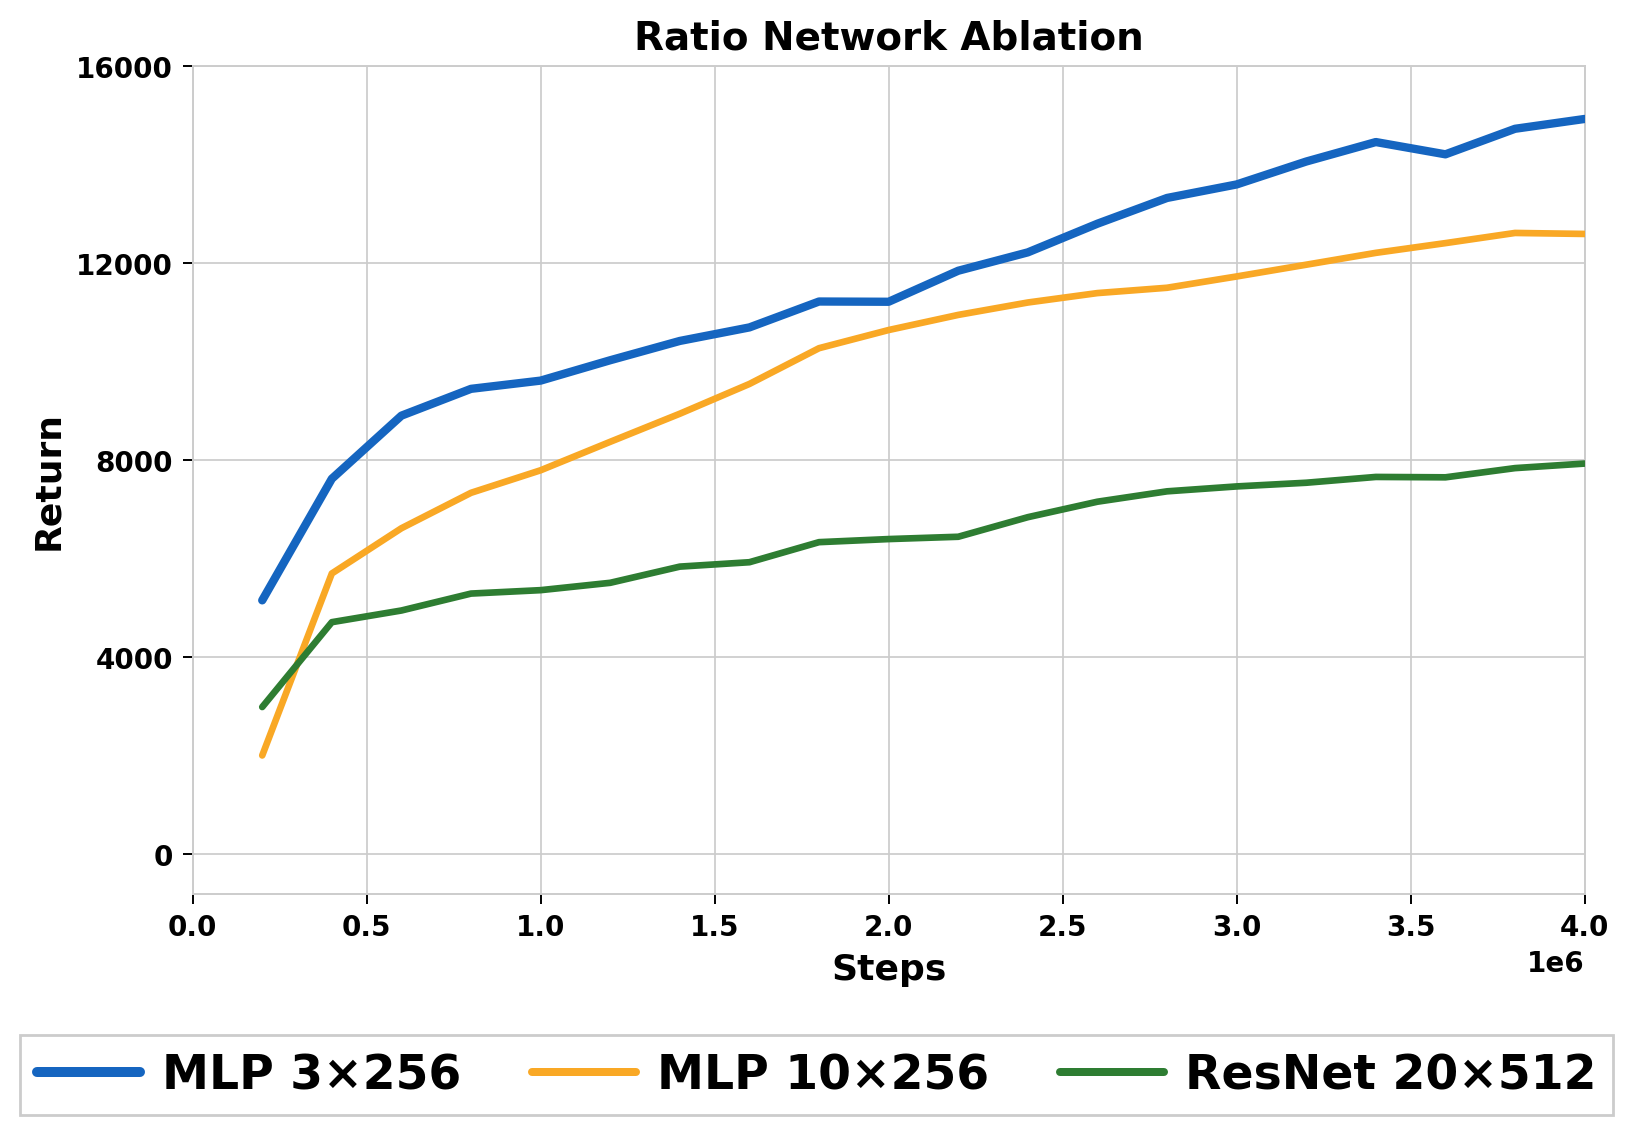
\includegraphics[width=\linewidth]{halfcheetah_ratio_ablation_red.png}
        \caption{\small Effect of ratio network architecture.}
    \end{subfigure}
    \hfill
    \begin{subfigure}{0.49\linewidth}
        \centering
        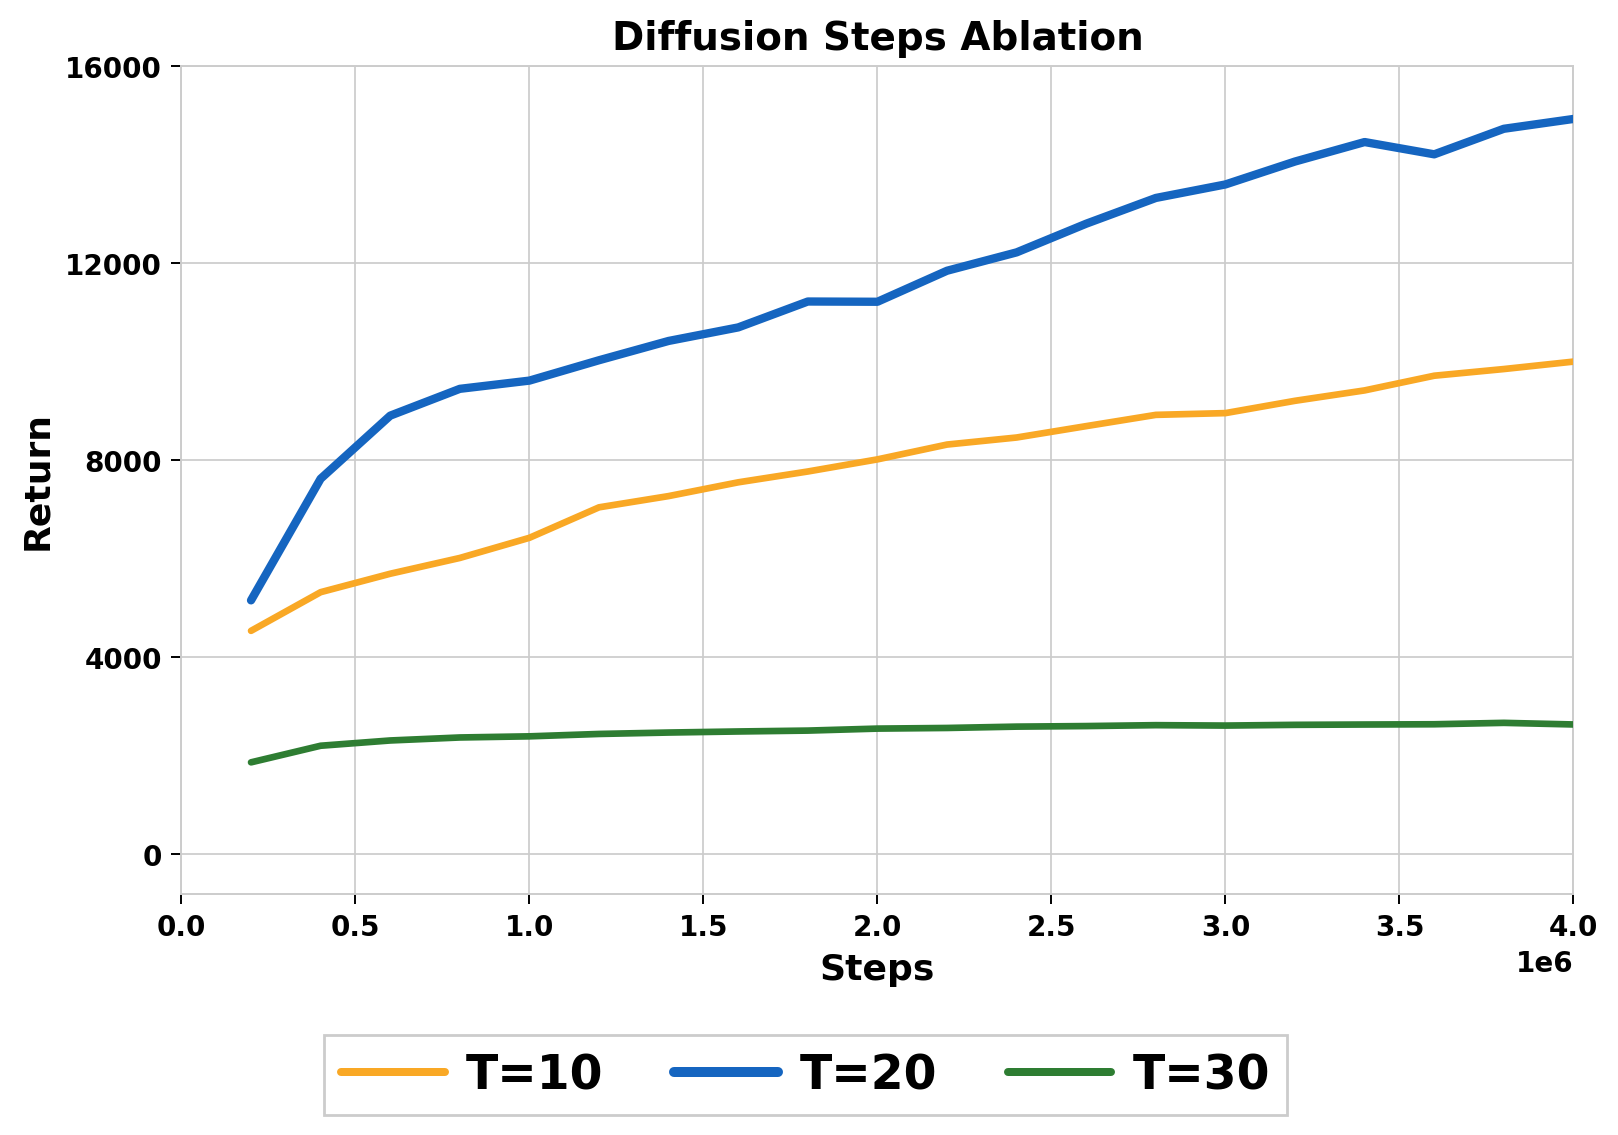
\includegraphics[width=\linewidth]{halfcheetah_diffusion_steps_ablation_red.png}
        \caption{\small Effect of the number of diffusion steps.}
    \end{subfigure}

    \vspace{-2mm}
    \caption{{\small Ablation study of DoobPPO on OpenAI Gym MuJoCo \texttt{HalfCheetah-v4}.
    \textbf{(a)} Effect of the ratio network architecture on policy performance.
    \textbf{(b)} Different diffusion steps lead to significantly different performance, with moderate steps performing best.}}
    \label{fig:ablation_two}
\end{figure}

\subsection{Diffusion Policy.}

\paragraph{Ablation Study on Ratio Network Size.}
We study the sensitivity of DoobPPO to the ratio-network architecture on \texttt{HalfCheetah-v4}.
We compare three variants: an MLP ratio network with 3 layers of width 256, a deeper MLP with 10 layers of width 256, and a larger ResNet-style architecture with 20 layers of width 512.
As shown in Figure~\ref{fig:ablation_two}, the simple 3$\times$256 MLP achieves the best performance, consistently outperforming both the deeper MLP and the larger ResNet-style model.
This suggests that increasing the capacity of the ratio network does not necessarily improve performance, and may even make optimization less effective.
Based on this result, we use the 3$\times$256 MLP ratio network in all diffusion-policy experiments.

\paragraph{Ablation Study on Diffusion Steps.}
We also study the sensitivity of DoobPPO to the number of diffusion steps on \texttt{HalfCheetah-v4}.
We compare three settings, namely $T=10$, $T=20$, and $T=30$.
The results show that $T=20$ achieves the best overall performance, while $T=10$ remains competitive but consistently underperforms $T=20$, and $T=30$ leads to a substantial degradation.
These results suggest that DoobPO benefits from a moderately sized diffusion process rather than a very shallow or overly long denoising chain.
Therefore, we use $20$ diffusion steps in all diffusion-policy experiments.

\subsection{Flow Policy.}

\begin{figure}[h]
    \centering
    \begin{subfigure}{0.49\linewidth}
        \centering
        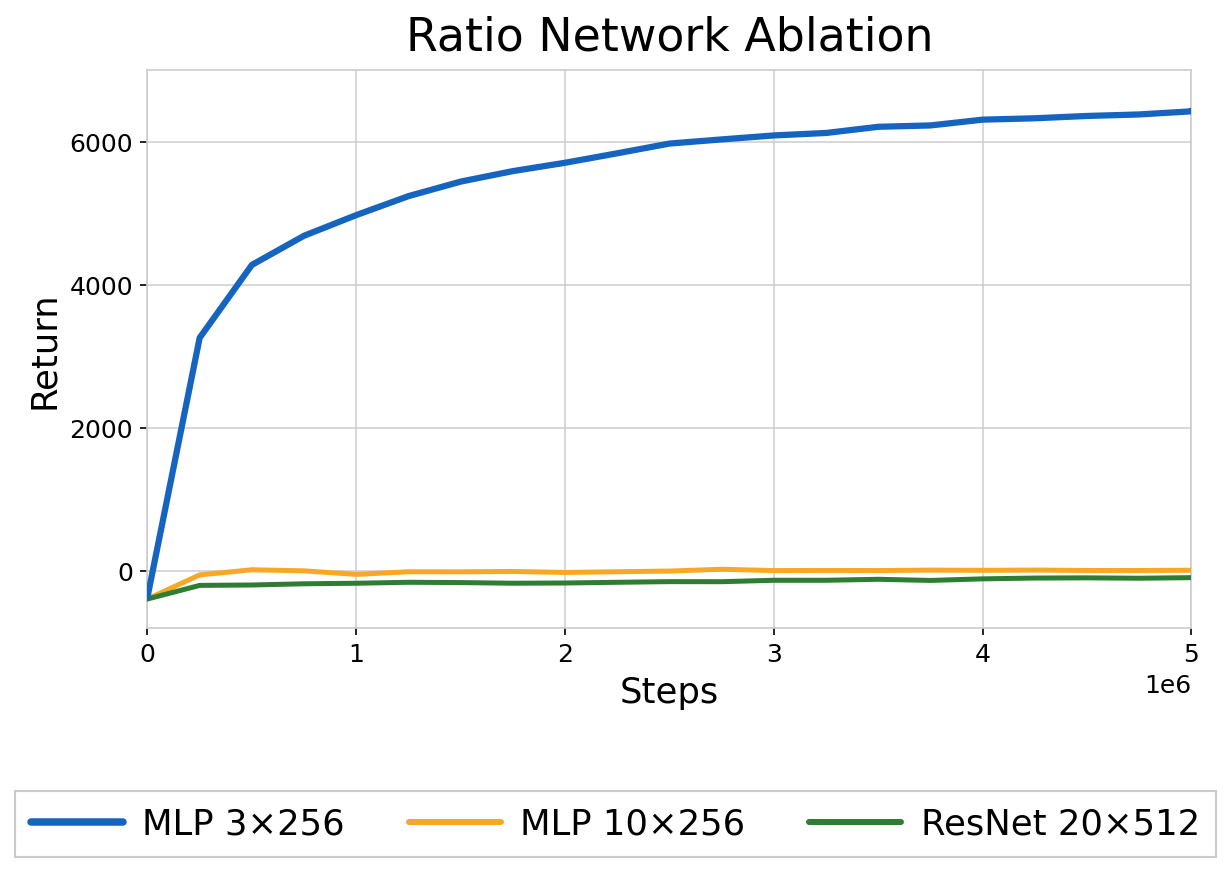
\includegraphics[width=\linewidth]{halfcheetah_flow_ratio_ablation_red.png}
        \caption{\small Effect of ratio network architecture.}
    \end{subfigure}
    \hfill
    \begin{subfigure}{0.49\linewidth}
        \centering
        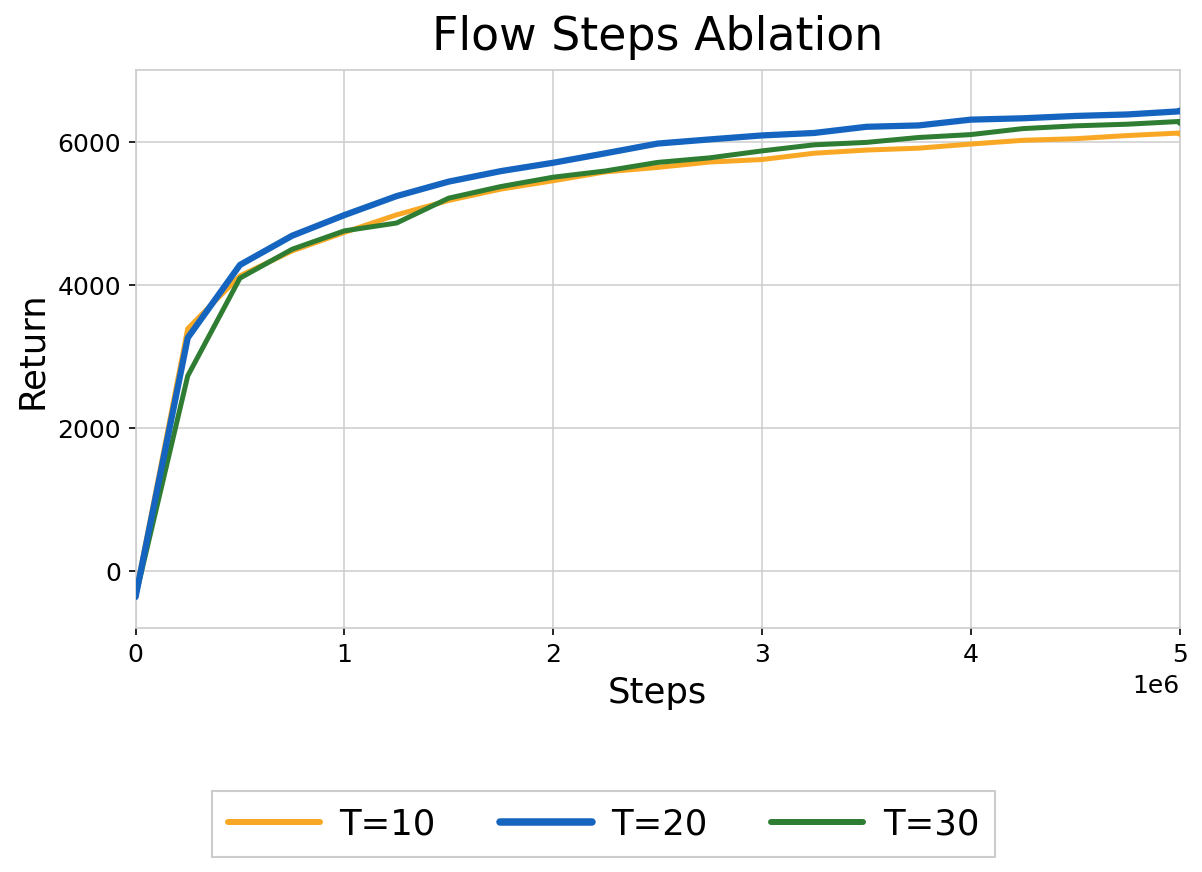
\includegraphics[width=\linewidth]{halfcheetah_flow_steps_ablation_red.png}
        \caption{\small Effect of the number of flow steps.}
    \end{subfigure}

    \vspace{-2mm}
    \caption{{\small Ablation study of DoobGRPO flow policy on OpenAI Gym MuJoCo \texttt{HalfCheetah-v4}.
    \textbf{(a)} Only the lightweight MLP 3$\times$256 ratio network learns effectively, while deeper and larger architectures fail to train.
    \textbf{(b)} Performance is robust to the number of flow steps, with $T{=}20$ achieving the best result and $T{=}10$, $T{=}30$ remaining competitive.}}
    \label{fig:ablation_flow}
\end{figure}

\paragraph{Ablation Study on Ratio Network Size.}
We study the sensitivity of DoobGRPO to the ratio-network architecture on \texttt{HalfCheetah-v4} with flow policies.
We compare the same three variants as in the diffusion-policy setting: an MLP ratio network with 3 layers of width 256, a deeper MLP with 10 layers of width 256, and a ResNet-style architecture with 20 blocks of width 512.
As shown in Figure~\ref{fig:ablation_flow}(a), the simple 3$\times$256 MLP achieves the best performance with a peak return of 6433, while both the deeper MLP (peak return 23) and the larger ResNet (peak return $-$94) fail to learn meaningful policies.
This is consistent with the diffusion-policy ablation, confirming that a lightweight ratio network is critical for stable training across both generative-model backbones.

\paragraph{Ablation Study on Flow Steps.}
We also study the sensitivity of DoobGRPO to the number of flow integration steps on \texttt{HalfCheetah-v4}.
We compare $T=10$, $T=20$, and $T=30$.
As shown in Figure~\ref{fig:ablation_flow}(b), the default setting $T=20$ achieves the best peak performance (6433), while $T=10$ (6120) and $T=30$ (6282) remain competitive but slightly underperform $T=20$.
These results suggest that DoobPO is relatively robust to the choice of flow steps, with $T=20$ providing the best trade-off between sampling quality and computational cost.
We use $20$ flow steps in all flow-policy experiments.


\clearpage
\section{Algorithms}

\subsection{Diffusion Policy Optimization with DoobPO}

\begin{algorithm}[h]
\caption{Diffusion Policy Optimization with DoobPO}
\label{alg:rwdm_ppo}
\begin{algorithmic}[1]
\Require Environment MDP $\mathcal{M}=(\mathcal{S},\mathcal{A},P,R,\gamma)$;
pre-trained score model $g_{\phi}$;
reinforcement learning objective $J_{\mathrm{RL}}$;
advantage estimator $\hat{A}$;
ratio network $r_\beta$;
ratio regularization coefficient $\lambda_{\mathrm{reg}}$;
iteration $K$
\State \textbf{Initialize:} drift model $\theta_1=\phi$; ratio net $\beta_1$.
\For{$k=1,2,\ldots,K$}
    \State Add rollout samples to replay buffer $\mathcal{D}$ from $\mathcal{M}$ using current policy $\pi^k$ induced by $g_{\theta_k}$
    \State Estimate advantage of current policy $A^{\pi^k}\leftarrow \hat{A}(\mathcal{D})$

    \State \textbf{Ratio learning update}
    \State Update $\beta$ by optimizing the regularized reinforcement learning objective
    \begin{align*}
        \beta_{k+1}
        \leftarrow
        \argmax_{\beta}
        \Big\{
        J_{\mathrm{RL}}(\beta)
        -
        \lambda_{\mathrm{reg}}
        \E_{o\sim\mathcal D}
        \Big[
        \big(
        \E_{a\sim \pi^k(\cdot|o)}[r_\beta(o,a)]-1
        \big)^2
        \Big]
        \Big\}.
    \end{align*}

    \State \textbf{Doob's drift matching update}
    \State For each $(o,a)\in\mathcal{D}$, sample $t\sim U[0,T]$ and generate noised action $x_t$
    \begin{align*}
        x_t \leftarrow \sqrt{\bar\alpha_t}\,a
    + \sqrt{1-\bar\alpha_t}\,z,
\quad z\sim\mathcal N(0,I)
    \end{align*}
    \State Update $\theta$ by minimizing the conditional drift matching objective
    \begin{align*}
        \theta_{k+1}\leftarrow \argmin_{\theta}
        \E_{(o,a,x_t,t)\sim\mathcal{D}}
        \Big[
        r_{\beta_{k+1}}(o,a)
        \Big\|
        -\frac{x_t-\sqrt{\bar\alpha_t}\,a}
    {1-\bar\alpha_t}
    -g_\theta(x_t,t,o)
        \Big\|_2^2
        \Big]
    \end{align*}
\EndFor
\State \textbf{Output:} Policy $\pi^{K+1}$ with learned drift $g_{\theta_{K+1}}$
\end{algorithmic}
\end{algorithm}


\clearpage
\subsection{Flow Policy Optimization with DoobPO}

\begin{algorithm}[h]
\caption{Flow Policy Optimization with DoobPO}
\label{alg:rwdm_ppo_fm}
\begin{algorithmic}[1]
\Require Environment MDP $\mathcal{M}=(\mathcal{S},\mathcal{A},P,R,\gamma)$;
pre-trained velocity model $u_{\phi}$;
reinforcement learning objective $J_{\mathrm{RL}}$;
advantage estimator $\hat{A}$;
ratio network $r_\beta$;
ratio regularization coefficient $\lambda_{\mathrm{reg}}$;
iteration $K$
\State \textbf{Initialize:} velocity model $\theta_1=\phi$; ratio net $\beta_1$.
\For{$k=1,2,\ldots,K$}
    \State Add rollout samples to replay buffer $\mathcal{D}$ from $\mathcal{M}$ using current policy $\pi^k$ induced by $u_{\theta_k}$
    \State Estimate advantage of current policy $A^{\pi^k}\leftarrow \hat{A}(\mathcal{D})$

    \State \textbf{Ratio learning update}
    \State Update $\beta$ by optimizing the regularized reinforcement learning objective
    \begin{align*}
        \beta_{k+1}
        \leftarrow
        \argmax_{\beta}
        \Big\{
        J_{\mathrm{RL}}(\beta)
        -
        \lambda_{\mathrm{reg}}
        \E_{o\sim\mathcal D}
        \Big[
        \big(
        \E_{a\sim \pi^k(\cdot|o)}[r_\beta(o,a)]-1
        \big)^2
        \Big]
        \Big\}.
    \end{align*}

    \State \textbf{Drift matching update}
    \State For each $(o,a)\in\mathcal{D}$, sample $t \sim U[0,T]$ and generate intermediate action $x_t$ by
    \begin{align*}
        x_t \leftarrow \alpha_t z
        + \beta_t a,
        \quad z \sim N(0,I)
    \end{align*}
    \State Update $\theta$ by minimizing the conditional drift matching objective
    \begin{align*}
        \theta_{k+1} \leftarrow \argmin_{\theta}
        \E_{(o,a,x_t,t)\sim \mathcal{D}}
        \Big[ r_{\beta_{k+1}}(o,a)\,
        \|
            \dot{\alpha}_t z + \dot{\beta}_t a
            - u_\theta(x_t,t,o)
        \|_2^2
        \Big]
    \end{align*}
\EndFor
\State \textbf{Output:} Policy $\pi^{K+1}$ with learned velocity $u_{\theta_{K+1}}$
\end{algorithmic}
\end{algorithm}


\clearpage
\section*{NeurIPS Paper Checklist}

%%% BEGIN INSTRUCTIONS %%%
% The checklist is designed to encourage best practices for responsible machine learning research, addressing issues of reproducibility, transparency, research ethics, and societal impact. Do not remove the checklist: {\bf The papers not including the checklist will be desk rejected.} The checklist should follow the references and follow the (optional) supplemental material.  The checklist does NOT count towards the page
% limit. 

% Please read the checklist guidelines carefully for information on how to answer these questions. For each question in the checklist:
% \begin{itemize}
%     \item You should answer \answerYes{}, \answerNo{}, or \answerNA{}.
%     \item \answerNA{} means either that the question is Not Applicable for that particular paper or the relevant information is Not Available.
%     \item Please provide a short (1--2 sentence) justification right after your answer (even for \answerNA). 
%    % \item {\bf The papers not including the checklist will be desk rejected.}
% \end{itemize}

% {\bf The checklist answers are an integral part of your paper submission.} They are visible to the reviewers, area chairs, senior area chairs, and ethics reviewers. You will also be asked to include it (after eventual revisions) with the final version of your paper, and its final version will be published with the paper.

% The reviewers of your paper will be asked to use the checklist as one of the factors in their evaluation. While \answerYes{} is generally preferable to \answerNo{}, it is perfectly acceptable to answer \answerNo{} provided a proper justification is given (e.g., error bars are not reported because it would be too computationally expensive'' or ``we were unable to find the license for the dataset we used''). In general, answering \answerNo{} or \answerNA{} is not grounds for rejection. While the questions are phrased in a binary way, we acknowledge that the true answer is often more nuanced, so please just use your best judgment and write a justification to elaborate. All supporting evidence can appear either in the main paper or the supplemental material, provided in appendix. If you answer \answerYes{} to a question, in the justification please point to the section(s) where related material for the question can be found.

% IMPORTANT, please:
% \begin{itemize}
%     \item {\bf Delete this instruction block, but keep the section heading ``NeurIPS Paper Checklist"},
%     \item  {\bf Keep the checklist subsection headings, questions/answers and guidelines below.}
%     \item {\bf Do not modify the questions and only use the provided macros for your answers}.
% \end{itemize} 
 

%%% END INSTRUCTIONS %%%


\begin{enumerate}

\item {\bf Claims}
    \item[] Question: Do the main claims made in the abstract and introduction accurately reflect the paper's contributions and scope?
    \item[] Answer: \answerYes{} % Replace by \answerYes{}, \answerNo{}, or \answerNA{}.
    \item[] Justification: All main claims are stated in the abstract, introduction, and theorem statements.
    \item[] Guidelines:
    \begin{itemize}
        \item The answer \answerNA{} means that the abstract and introduction do not include the claims made in the paper.
        \item The abstract and/or introduction should clearly state the claims made, including the contributions made in the paper and important assumptions and limitations. A \answerNo{} or \answerNA{} answer to this question will not be perceived well by the reviewers. 
        \item The claims made should match theoretical and experimental results, and reflect how much the results can be expected to generalize to other settings. 
        \item It is fine to include aspirational goals as motivation as long as it is clear that these goals are not attained by the paper. 
    \end{itemize}

\item {\bf Limitations}
    \item[] Question: Does the paper discuss the limitations of the work performed by the authors?
    \item[] Answer: \answerYes{} % Replace by \answerYes{}, \answerNo{}, or \answerNA{}.
    \item[] Justification:
    We discuss limitations in \cref{sec:conclusion}.
    We discuss the method now only support continuous generation.
    We may extend this to discrete setting.
    \item[] Guidelines:
    \begin{itemize}
        \item The answer \answerNA{} means that the paper has no limitation while the answer \answerNo{} means that the paper has limitations, but those are not discussed in the paper. 
        \item The authors are encouraged to create a separate ``Limitations'' section in their paper.
        \item The paper should point out any strong assumptions and how robust the results are to violations of these assumptions (e.g., independence assumptions, noiseless settings, model well-specification, asymptotic approximations only holding locally). The authors should reflect on how these assumptions might be violated in practice and what the implications would be.
        \item The authors should reflect on the scope of the claims made, e.g., if the approach was only tested on a few datasets or with a few runs. In general, empirical results often depend on implicit assumptions, which should be articulated.
        \item The authors should reflect on the factors that influence the performance of the approach. For example, a facial recognition algorithm may perform poorly when image resolution is low or images are taken in low lighting. Or a speech-to-text system might not be used reliably to provide closed captions for online lectures because it fails to handle technical jargon.
        \item The authors should discuss the computational efficiency of the proposed algorithms and how they scale with dataset size.
        \item If applicable, the authors should discuss possible limitations of their approach to address problems of privacy and fairness.
        \item While the authors might fear that complete honesty about limitations might be used by reviewers as grounds for rejection, a worse outcome might be that reviewers discover limitations that aren't acknowledged in the paper. The authors should use their best judgment and recognize that individual actions in favor of transparency play an important role in developing norms that preserve the integrity of the community. Reviewers will be specifically instructed to not penalize honesty concerning limitations.
    \end{itemize}

\item {\bf Theory assumptions and proofs}
    \item[] Question: For each theoretical result, does the paper provide the full set of assumptions and a complete (and correct) proof?
    \item[] Answer: \answerYes{} % Replace by \answerYes{}, \answerNo{}, or \answerNA{}.
    \item[] Justification:
    All assumptions are stated in the main text, and complete proofs are provided in the appendix.
    \item[] Guidelines:
    \begin{itemize}
        \item The answer \answerNA{} means that the paper does not include theoretical results. 
        \item All the theorems, formulas, and proofs in the paper should be numbered and cross-referenced.
        \item All assumptions should be clearly stated or referenced in the statement of any theorems.
        \item The proofs can either appear in the main paper or the supplemental material, but if they appear in the supplemental material, the authors are encouraged to provide a short proof sketch to provide intuition. 
        \item Inversely, any informal proof provided in the core of the paper should be complemented by formal proofs provided in appendix or supplemental material.
        \item Theorems and Lemmas that the proof relies upon should be properly referenced. 
    \end{itemize}

    \item {\bf Experimental result reproducibility}
    \item[] Question: Does the paper fully disclose all the information needed to reproduce the main experimental results of the paper to the extent that it affects the main claims and/or conclusions of the paper (regardless of whether the code and data are provided or not)?
    \item[] Answer: \answerYes{} % Replace by \answerYes{}, \answerNo{}, or \answerNA{}.
    \item[] Justification: We fully disclose all the information needed.
    \item[] Guidelines:
    \begin{itemize}
        \item The answer \answerNA{} means that the paper does not include experiments.
        \item If the paper includes experiments, a \answerNo{} answer to this question will not be perceived well by the reviewers: Making the paper reproducible is important, regardless of whether the code and data are provided or not.
        \item If the contribution is a dataset and\slash or model, the authors should describe the steps taken to make their results reproducible or verifiable. 
        \item Depending on the contribution, reproducibility can be accomplished in various ways. For example, if the contribution is a novel architecture, describing the architecture fully might suffice, or if the contribution is a specific model and empirical evaluation, it may be necessary to either make it possible for others to replicate the model with the same dataset, or provide access to the model. In general. releasing code and data is often one good way to accomplish this, but reproducibility can also be provided via detailed instructions for how to replicate the results, access to a hosted model (e.g., in the case of a large language model), releasing of a model checkpoint, or other means that are appropriate to the research performed.
        \item While NeurIPS does not require releasing code, the conference does require all submissions to provide some reasonable avenue for reproducibility, which may depend on the nature of the contribution. For example
        \begin{enumerate}
            \item If the contribution is primarily a new algorithm, the paper should make it clear how to reproduce that algorithm.
            \item If the contribution is primarily a new model architecture, the paper should describe the architecture clearly and fully.
            \item If the contribution is a new model (e.g., a large language model), then there should either be a way to access this model for reproducing the results or a way to reproduce the model (e.g., with an open-source dataset or instructions for how to construct the dataset).
            \item We recognize that reproducibility may be tricky in some cases, in which case authors are welcome to describe the particular way they provide for reproducibility. In the case of closed-source models, it may be that access to the model is limited in some way (e.g., to registered users), but it should be possible for other researchers to have some path to reproducing or verifying the results.
        \end{enumerate}
    \end{itemize}


\item {\bf Open access to data and code}
    \item[] Question: Does the paper provide open access to the data and code, with sufficient instructions to faithfully reproduce the main experimental results, as described in supplemental material?
    \item[] Answer: \answerYes{} % Replace by \answerYes{}, \answerNo{}, or \answerNA{}.
    \item[] Justification: We show the details of experiments in the paper and we submit the code in the supplemental material.
    \item[] Guidelines:
    \begin{itemize}
        \item The answer \answerNA{} means that paper does not include experiments requiring code.
        \item Please see the NeurIPS code and data submission guidelines (\url{https://neurips.cc/public/guides/CodeSubmissionPolicy}) for more details.
        \item While we encourage the release of code and data, we understand that this might not be possible, so \answerNo{} is an acceptable answer. Papers cannot be rejected simply for not including code, unless this is central to the contribution (e.g., for a new open-source benchmark).
        \item The instructions should contain the exact command and environment needed to run to reproduce the results. See the NeurIPS code and data submission guidelines (\url{https://neurips.cc/public/guides/CodeSubmissionPolicy}) for more details.
        \item The authors should provide instructions on data access and preparation, including how to access the raw data, preprocessed data, intermediate data, and generated data, etc.
        \item The authors should provide scripts to reproduce all experimental results for the new proposed method and baselines. If only a subset of experiments are reproducible, they should state which ones are omitted from the script and why.
        \item At submission time, to preserve anonymity, the authors should release anonymized versions (if applicable).
        \item Providing as much information as possible in supplemental material (appended to the paper) is recommended, but including URLs to data and code is permitted.
    \end{itemize}


\item {\bf Experimental setting/details}
    \item[] Question: Does the paper specify all the training and test details (e.g., data splits, hyperparameters, how they were chosen, type of optimizer) necessary to understand the results?
    \item[] Answer: \answerYes{} % Replace by \answerYes{}, \answerNo{}, or \answerNA{}.
    \item[] Justification: The paper describes the model setting in \cref{sec:exp} and \cref{sec:implementation}.
    \item[] Guidelines:
    \begin{itemize}
        \item The answer \answerNA{} means that the paper does not include experiments.
        \item The experimental setting should be presented in the core of the paper to a level of detail that is necessary to appreciate the results and make sense of them.
        \item The full details can be provided either with the code, in appendix, or as supplemental material.
    \end{itemize}

\item {\bf Experiment statistical significance}
    \item[] Question: Does the paper report error bars suitably and correctly defined or other appropriate information about the statistical significance of the experiments?
    \item[] Answer: \answerYes{} % Replace by \answerYes{}, \answerNo{}, or \answerNA{}.
    \item[] Justification: We run the experiments with different seeds and report the mean and std. 
    \item[] Guidelines:
    \begin{itemize}
        \item The answer \answerNA{} means that the paper does not include experiments.
        \item The authors should answer \answerYes{} if the results are accompanied by error bars, confidence intervals, or statistical significance tests, at least for the experiments that support the main claims of the paper.
        \item The factors of variability that the error bars are capturing should be clearly stated (for example, train/test split, initialization, random drawing of some parameter, or overall run with given experimental conditions).
        \item The method for calculating the error bars should be explained (closed form formula, call to a library function, bootstrap, etc.)
        \item The assumptions made should be given (e.g., Normally distributed errors).
        \item It should be clear whether the error bar is the standard deviation or the standard error of the mean.
        \item It is OK to report 1-sigma error bars, but one should state it. The authors should preferably report a 2-sigma error bar than state that they have a 96\% CI, if the hypothesis of Normality of errors is not verified.
        \item For asymmetric distributions, the authors should be careful not to show in tables or figures symmetric error bars that would yield results that are out of range (e.g., negative error rates).
        \item If error bars are reported in tables or plots, the authors should explain in the text how they were calculated and reference the corresponding figures or tables in the text.
    \end{itemize}

\item {\bf Experiments compute resources}
    \item[] Question: For each experiment, does the paper provide sufficient information on the computer resources (type of compute workers, memory, time of execution) needed to reproduce the experiments?
    \item[] Answer: \answerYes{} % Replace by \answerYes{}, \answerNo{}, or \answerNA{}.
    \item[] Justification: We have mentioned all information about compute resources in \cref{sec:implementation}.
    \item[] Guidelines:
    \begin{itemize}
        \item The answer \answerNA{} means that the paper does not include experiments.
        \item The paper should indicate the type of compute workers CPU or GPU, internal cluster, or cloud provider, including relevant memory and storage.
        \item The paper should provide the amount of compute required for each of the individual experimental runs as well as estimate the total compute. 
        \item The paper should disclose whether the full research project required more compute than the experiments reported in the paper (e.g., preliminary or failed experiments that didn't make it into the paper). 
    \end{itemize}
    
\item {\bf Code of ethics}
    \item[] Question: Does the research conducted in the paper conform, in every respect, with the NeurIPS Code of Ethics \url{https://neurips.cc/public/EthicsGuidelines}?
    \item[] Answer: \answerYes{} % Replace by \answerYes{}, \answerNo{}, or \answerNA{}.
    \item[] Justification: We reviewed the NeurIPS Code of Ethics and believe the research conforms to it. 
    \item[] Guidelines:
    \begin{itemize}
        \item The answer \answerNA{} means that the authors have not reviewed the NeurIPS Code of Ethics.
        \item If the authors answer \answerNo, they should explain the special circumstances that require a deviation from the Code of Ethics.
        \item The authors should make sure to preserve anonymity (e.g., if there is a special consideration due to laws or regulations in their jurisdiction).
    \end{itemize}


\item {\bf Broader impacts}
    \item[] Question: Does the paper discuss both potential positive societal impacts and negative societal impacts of the work performed?
    \item[] Answer: \answerYes{} % Replace by \answerYes{}, \answerNo{}, or \answerNA{}.
    \item[] Justification: The paper includes an ethics statement and discusses the likely scope of the work.
    \item[] Guidelines:
    \begin{itemize}
        \item The answer \answerNA{} means that there is no societal impact of the work performed.
        \item If the authors answer \answerNA{} or \answerNo, they should explain why their work has no societal impact or why the paper does not address societal impact.
        \item Examples of negative societal impacts include potential malicious or unintended uses (e.g., disinformation, generating fake profiles, surveillance), fairness considerations (e.g., deployment of technologies that could make decisions that unfairly impact specific groups), privacy considerations, and security considerations.
        \item The conference expects that many papers will be foundational research and not tied to particular applications, let alone deployments. However, if there is a direct path to any negative applications, the authors should point it out. For example, it is legitimate to point out that an improvement in the quality of generative models could be used to generate Deepfakes for disinformation. On the other hand, it is not needed to point out that a generic algorithm for optimizing neural networks could enable people to train models that generate Deepfakes faster.
        \item The authors should consider possible harms that could arise when the technology is being used as intended and functioning correctly, harms that could arise when the technology is being used as intended but gives incorrect results, and harms following from (intentional or unintentional) misuse of the technology.
        \item If there are negative societal impacts, the authors could also discuss possible mitigation strategies (e.g., gated release of models, providing defenses in addition to attacks, mechanisms for monitoring misuse, mechanisms to monitor how a system learns from feedback over time, improving the efficiency and accessibility of ML).
    \end{itemize}
    
\item {\bf Safeguards}
    \item[] Question: Does the paper describe safeguards that have been put in place for responsible release of data or models that have a high risk for misuse (e.g., pre-trained language models, image generators, or scraped datasets)?
    \item[] Answer: \answerNA{} % Replace by \answerYes{}, \answerNo{}, or \answerNA{}.
    \item[] Justification: The paper does not release high-risk datasets, pre-trained models, or generative systems that require special safeguards. 
    \item[] Guidelines:
    \begin{itemize}
        \item The answer \answerNA{} means that the paper poses no such risks.
        \item Released models that have a high risk for misuse or dual-use should be released with necessary safeguards to allow for controlled use of the model, for example by requiring that users adhere to usage guidelines or restrictions to access the model or implementing safety filters. 
        \item Datasets that have been scraped from the Internet could pose safety risks. The authors should describe how they avoided releasing unsafe images.
        \item We recognize that providing effective safeguards is challenging, and many papers do not require this, but we encourage authors to take this into account and make a best faith effort.
    \end{itemize}

\item {\bf Licenses for existing assets}
    \item[] Question: Are the creators or original owners of assets (e.g., code, data, models), used in the paper, properly credited and are the license and terms of use explicitly mentioned and properly respected?
    \item[] Answer: \answerYes{} % Replace by \answerYes{}, \answerNo{}, or \answerNA{}.
    \item[] Justification:  All external assets used in this work are credited and used in accordance with their licenses. 
    \item[] Guidelines:
    \begin{itemize}
        \item The answer \answerNA{} means that the paper does not use existing assets.
        \item The authors should cite the original paper that produced the code package or dataset.
        \item The authors should state which version of the asset is used and, if possible, include a URL.
        \item The name of the license (e.g., CC-BY 4.0) should be included for each asset.
        \item For scraped data from a particular source (e.g., website), the copyright and terms of service of that source should be provided.
        \item If assets are released, the license, copyright information, and terms of use in the package should be provided. For popular datasets, \url{paperswithcode.com/datasets} has curated licenses for some datasets. Their licensing guide can help determine the license of a dataset.
        \item For existing datasets that are re-packaged, both the original license and the license of the derived asset (if it has changed) should be provided.
        \item If this information is not available online, the authors are encouraged to reach out to the asset's creators.
    \end{itemize}

\item {\bf New assets}
    \item[] Question: Are new assets introduced in the paper well documented and is the documentation provided alongside the assets?
    \item[] Answer: \answerYes{} % Replace by \answerYes{}, \answerNo{}, or \answerNA{}.
    \item[] Justification: All new assets introduced in the paper are well documented.
    \item[] Guidelines:
    \begin{itemize}
        \item The answer \answerNA{} means that the paper does not release new assets.
        \item Researchers should communicate the details of the dataset\slash code\slash model as part of their submissions via structured templates. This includes details about training, license, limitations, etc. 
        \item The paper should discuss whether and how consent was obtained from people whose asset is used.
        \item At submission time, remember to anonymize your assets (if applicable). You can either create an anonymized URL or include an anonymized zip file.
    \end{itemize}

\item {\bf Crowdsourcing and research with human subjects}
    \item[] Question: For crowdsourcing experiments and research with human subjects, does the paper include the full text of instructions given to participants and screenshots, if applicable, as well as details about compensation (if any)? 
    \item[] Answer: \answerNA{} % Replace by \answerYes{}, \answerNo{}, or \answerNA{}.
    \item[] Justification: The paper does not involve crowdsourcing experiments or research with human subjects.
    \item[] Guidelines:
    \begin{itemize}
        \item The answer \answerNA{} means that the paper does not involve crowdsourcing nor research with human subjects.
        \item Including this information in the supplemental material is fine, but if the main contribution of the paper involves human subjects, then as much detail as possible should be included in the main paper. 
        \item According to the NeurIPS Code of Ethics, workers involved in data collection, curation, or other labor should be paid at least the minimum wage in the country of the data collector. 
    \end{itemize}

\item {\bf Institutional review board (IRB) approvals or equivalent for research with human subjects}
    \item[] Question: Does the paper describe potential risks incurred by study participants, whether such risks were disclosed to the subjects, and whether Institutional Review Board (IRB) approvals (or an equivalent approval/review based on the requirements of your country or institution) were obtained?
    \item[] Answer: \answerNA{} % Replace by \answerYes{}, \answerNo{}, or \answerNA{}.
    \item[] Justification: The paper does not involve crowdsourcing or research with human subjects.
    \item[] Guidelines:
    \begin{itemize}
        \item The answer \answerNA{} means that the paper does not involve crowdsourcing nor research with human subjects.
        \item Depending on the country in which research is conducted, IRB approval (or equivalent) may be required for any human subjects research. If you obtained IRB approval, you should clearly state this in the paper. 
        \item We recognize that the procedures for this may vary significantly between institutions and locations, and we expect authors to adhere to the NeurIPS Code of Ethics and the guidelines for their institution. 
        \item For initial submissions, do not include any information that would break anonymity (if applicable), such as the institution conducting the review.
    \end{itemize}

\item {\bf Declaration of LLM usage}
    \item[] Question: Does the paper describe the usage of LLMs if it is an important, original, or non-standard component of the core methods in this research? Note that if the LLM is used only for writing, editing, or formatting purposes and does \emph{not} impact the core methodology, scientific rigor, or originality of the research, declaration is not required.
    %this research? 
    \item[] Answer: \answerNA{} % Replace by \answerYes{}, \answerNo{}, or \answerNA{}.
    \item[] Justification: We describe the usage of LLMs in the appendix.
    \item[] Guidelines:
    \begin{itemize}
        \item The answer \answerNA{} means that the core method development in this research does not involve LLMs as any important, original, or non-standard components.
        \item Please refer to our LLM policy in the NeurIPS handbook for what should or should not be described.
    \end{itemize}

\end{enumerate}
\end{document}